\documentclass[compress]{beamer}
% Useful for large documents with lots of images: [draft]

%
% Other possibilities exist for notes, e.g.:
% \usepackage{pgfpages}
% \setbeameroption{show notes on second screen}
%\setbeameroption{show notes}


\usepackage{etex} %helps when using lots of packages
\mode<presentation>

\usepackage{amsmath}
\usepackage{amsthm}

%%%%%%%%%%%%%%%%%%%%%%%%%%%%%%%%%%%%%%%%
                                       %
% change this line for portable code:  %
\newcommand*{\commonDir}{./common/}%
\input{\commonDir preambleCommon}      %
                                       %
%%%%%%%%%%%%%%%%%%%%%%%%%%%%%%%%%%%%%%%%

\usepackage{listings}
\usepackage{atslistings}
\usepackage[bigfiles]{media9}
\usepackage{stfloats}
\captionsetup[figure]{labelformat=empty}

\graphicspath{{\commonDir figuresFalconTalk/}{./falcon/figures/}%
{./epistasisSameGene/figures/}{./thesis/figures/}%
{./epistasisBeneficialMutant/figures/}%
}

%%%%%%%%%%%%%%%%%%%%%%%%%%%%%%%
                              %
\input{\commonDir logos}      %
                              %
%%%%%%%%%%%%%%%%%%%%%%%%%%%%%%%


\usetheme{Warsaw}
% other themes: AnnArbor, Antibes, Bergen, Berkeley, Berlin, Boadilla, boxes, CambridgeUS, Copenhagen, Darmstadt, default, Dresden, Frankfurt, Goettingen,
% Hannover, Ilmenau, JuanLesPins, Luebeck, Madrid, Maloe, Marburg, Montpellier, PaloAlto, Pittsburg, Rochester, Singapore, Szeged, classic

%\usecolortheme{lily}
% color themes: albatross, beaver, beetle, crane, default, dolphin, dov, fly, lily, orchid, rose, seagull, seahorse, sidebartab, structure, whale, wolverine

%\usefonttheme{serif}
% font themes: default, professionalfonts, serif, structurebold, structureitalicserif, structuresmallcapsserif

\hypersetup{pdfpagemode=FullScreen} % makes your presentation go automatically to full screen

% define your own colors:
\definecolor{CURed}{rgb}{0.702,0.106,0.106}
\definecolor{CUGrey}{rgb}{0.302,0.31,0.3255}
%
\definecolor{White}{rgb}{1,1,1}
\definecolor{Red}{rgb}{1,0,0}
\definecolor{Blue}{rgb}{0,0,1}
\definecolor{Green}{rgb}{0,1,0}
\definecolor{Yellow}{rgb}{1,1,0}
\definecolor{magenta}{rgb}{1,0,.6}
\definecolor{lightblue}{rgb}{0,.5,1}
\definecolor{lightpurple}{rgb}{.6,.4,1}
\definecolor{gold}{rgb}{.6,.5,0}
\definecolor{orange}{rgb}{1,0.4,0}
\definecolor{hotpink}{rgb}{1,0,0.5}
\definecolor{newcolor2}{rgb}{.5,.3,.5}
\definecolor{newcolor}{rgb}{0,.3,1}
\definecolor{newcolor3}{rgb}{1,0,.35}
\definecolor{darkgreen1}{rgb}{0, .35, 0}
\definecolor{darkgreen}{rgb}{0, .6, 0}
\definecolor{darkred}{rgb}{.75,0,0}

\xdefinecolor{olive}{cmyk}{0.64,0,0.95,0.4}
\xdefinecolor{purpleish}{cmyk}{0.75,0.75,0,0}

% can also choose different themes for the "inside" and "outside"

% \usepackage{beamerinnertheme_______}
% inner themes include circles, default, inmargin, rectangles, rounded

% \usepackage{beamerouterthemesmoothbars}
% outer themes include default, infolines, miniframes, shadow, sidebar, smoothbars, smoothtree, split, tree

\useoutertheme[subsection=false]{smoothbars}

% to have the same footer on all slides
%\setbeamertemplate{footline}[text line]{STUFF HERE!}
\setbeamertemplate{footline}[text line]{} % makes the footer EMPTY

% Change some colors:
\setbeamercolor{structure}{fg=CURed}
\setbeamercolor{local structure}{fg=CURed}
\setbeamercolor{block title}{bg=CURed}
\setbeamercolor{block body}{bg=CURed!10}
\setbeamercolor*{palette quaternary}{fg=white,bg=CUGrey}


% include packages
\usepackage{multicol}
\usepackage[all,knot]{xy}
\xyoption{arc}
\usepackage{url}
\usepackage{hyperref}
\usepackage{picture}
%\usepackage{bmpsize}
     
%%%%%%%%%%%%%%%%%%%%%%%%%%%%%%%%%%%%%%%%%%%%%%%%%%%%%%%%%%%%%%%%%%%%%%%%%%%%%%%%%%%%%%%%%%
%%%%%%%%%%%%%%%%%%%%%%%%%%%%%% Title Page Info %%%%%%%%%%%%%%%%%%%%%%%%%%%%%%%%%%%%%%%%%%%
%%%%%%%%%%%%%%%%%%%%%%%%%%%%%%%%%%%%%%%%%%%%%%%%%%%%%%%%%%%%%%%%%%%%%%%%%%%%%%%%%%%%%%%%%%

\title{Advances in Genome-Scale Modeling Applied to Expression-based
Flux Estimation and Epistasis Prediction}
\author{\texorpdfstring{Brandon Barker\newline
  \url{brandon.barker@gmail.com}}{Brandon Barker}}
\institute{
Tri-Institutional Program in Computational Biology and Medicine\\ 
Gu Laboratory\\
Cornell University \\ \vspace{.25cm}B Exam Dissertation}
\date{\today}

%%%%%%%%%%%%%%%%%%%%%%%%%%%%%%%%%%%%%%%%%%%%%%%%%%%%%%%%%%%%%%%%%%%%%%%%%%%%%%%%%%%%%%%%%%
%%%%%%%%%%%%%%%%%%%%%%%%%%%%%% Begin Your Document %%%%%%%%%%%%%%%%%%%%%%%%%%%%%%%%%%%%%%%
%%%%%%%%%%%%%%%%%%%%%%%%%%%%%%%%%%%%%%%%%%%%%%%%%%%%%%%%%%%%%%%%%%%%%%%%%%%%%%%%%%%%%%%%%%


\begin{document}

%%%%%%%%%%%%%%%%%%%%%%%%%%%%%%%%%%%%%%%%
                                       %
\newboolean{thesisStyle}               %
\setboolean{thesisStyle}{true}         %
                                       %
\input{\commonDir documentHeadCommon}  %
                                       %
%%%%%%%%%%%%%%%%%%%%%%%%%%%%%%%%%%%%%%%%

%\newcommand\Small{\fontsize{9}{9.2}\selectfont}
%\newcommand*\LSTfont{\scriptsize\ttfamily\SetTracking{encoding=*}{-60}\lsstyle}

%%%%%%%%%%%%%%%%%%%%%%%%%%%%%%%%%%%%%%%%%%%%%%%%%%%%%%%%%%%%%%%%%%%%%%%%%%%%%%%%%%%%%%%%%%

\frame{
  \titlepage 
}

\note{
\scriptsize
``   `` Thank you. It's been good meeting everyone
so far and I look forward to talking with all of you later in the
day. I'm a student in the Tri-Institutional program in
Computational Biology and Medicine, which has associations
with the Weill Cornell Medical School and Memorial Sloan-Kettering
in NYC.
\par

I'm graduating from Zhenglong Gu's laboratory in Nutritional Sciences
- one of the computational groups in Biology at Cornell.  Our goal in
this research and much of my thesis is to build tools enabling the
computation of a fundamental metabolic quantity, called flux, in
models that may help us to understand disease as well as various
microbial interactions. In this presentation I will mainly be
discussing a recent project that we've been working on for about a
year and a half related to modeling metabolism of whole cells, but
before we get in to that, I just want to briefly introduce my
computational history.
\par
}

%%%%%%%%%%%%%%%%%%%%%%%%%%%%%%%%%%%%%%%%%%%%%%%%%%%%%%%%%%%%%%%%%%%%%%%%%%%%%%%%%%%%%%%%%%
% this puts the outline before EACH section automatically & will
% highlight the section you're about to talk about
%\section[Outline]{}
%\frame{\tableofcontents}

%%%%%%%%%%%%%%%%%%%%%%%%%%%%%%%%%%%%%%%%%%%%%%%%%%%%%%%%%%%%%%%%%%%%%%%%%%%%%%%%%%%%%%%%%%


%%%%%%%%%%%%%%%%%%%%%%%%%
                        %
\section{Introduction}  %
\subsection{Gene rules} %
                        %
%%%%%%%%%%%%%%%%%%%%%%%%%


%%%%%%%%%%%%%%%%%%%%%%%%%%%%%%%%%%%%%%%%%%%%%%%%%%%%%%%%%%%%%%%%%%%%%%%%%%%%%%%%%%%%%%%%%%

\newcommand{\introduceFlux}{%
\begin{block}{Flux}
\small
rate at which a reaction occurs\\
\vspace{1ex}\hrule\vspace{1ex}
\textit{throughput of cars on a road}
\end{block}

\begin{block}{Enzyme}
\small
protein catalyst that increase the flux for its
associated reactions\\
\vspace{1ex}\hrule\vspace{1ex}
\textit{the width of the road}\\
\end{block}
}

\newcommand{\introduceFluxTitle}
  {Metabolic pathways and their components}

\frame{\frametitle{\introduceFluxTitle}
\begin{columns}
\begin{column}{0.55\textwidth}
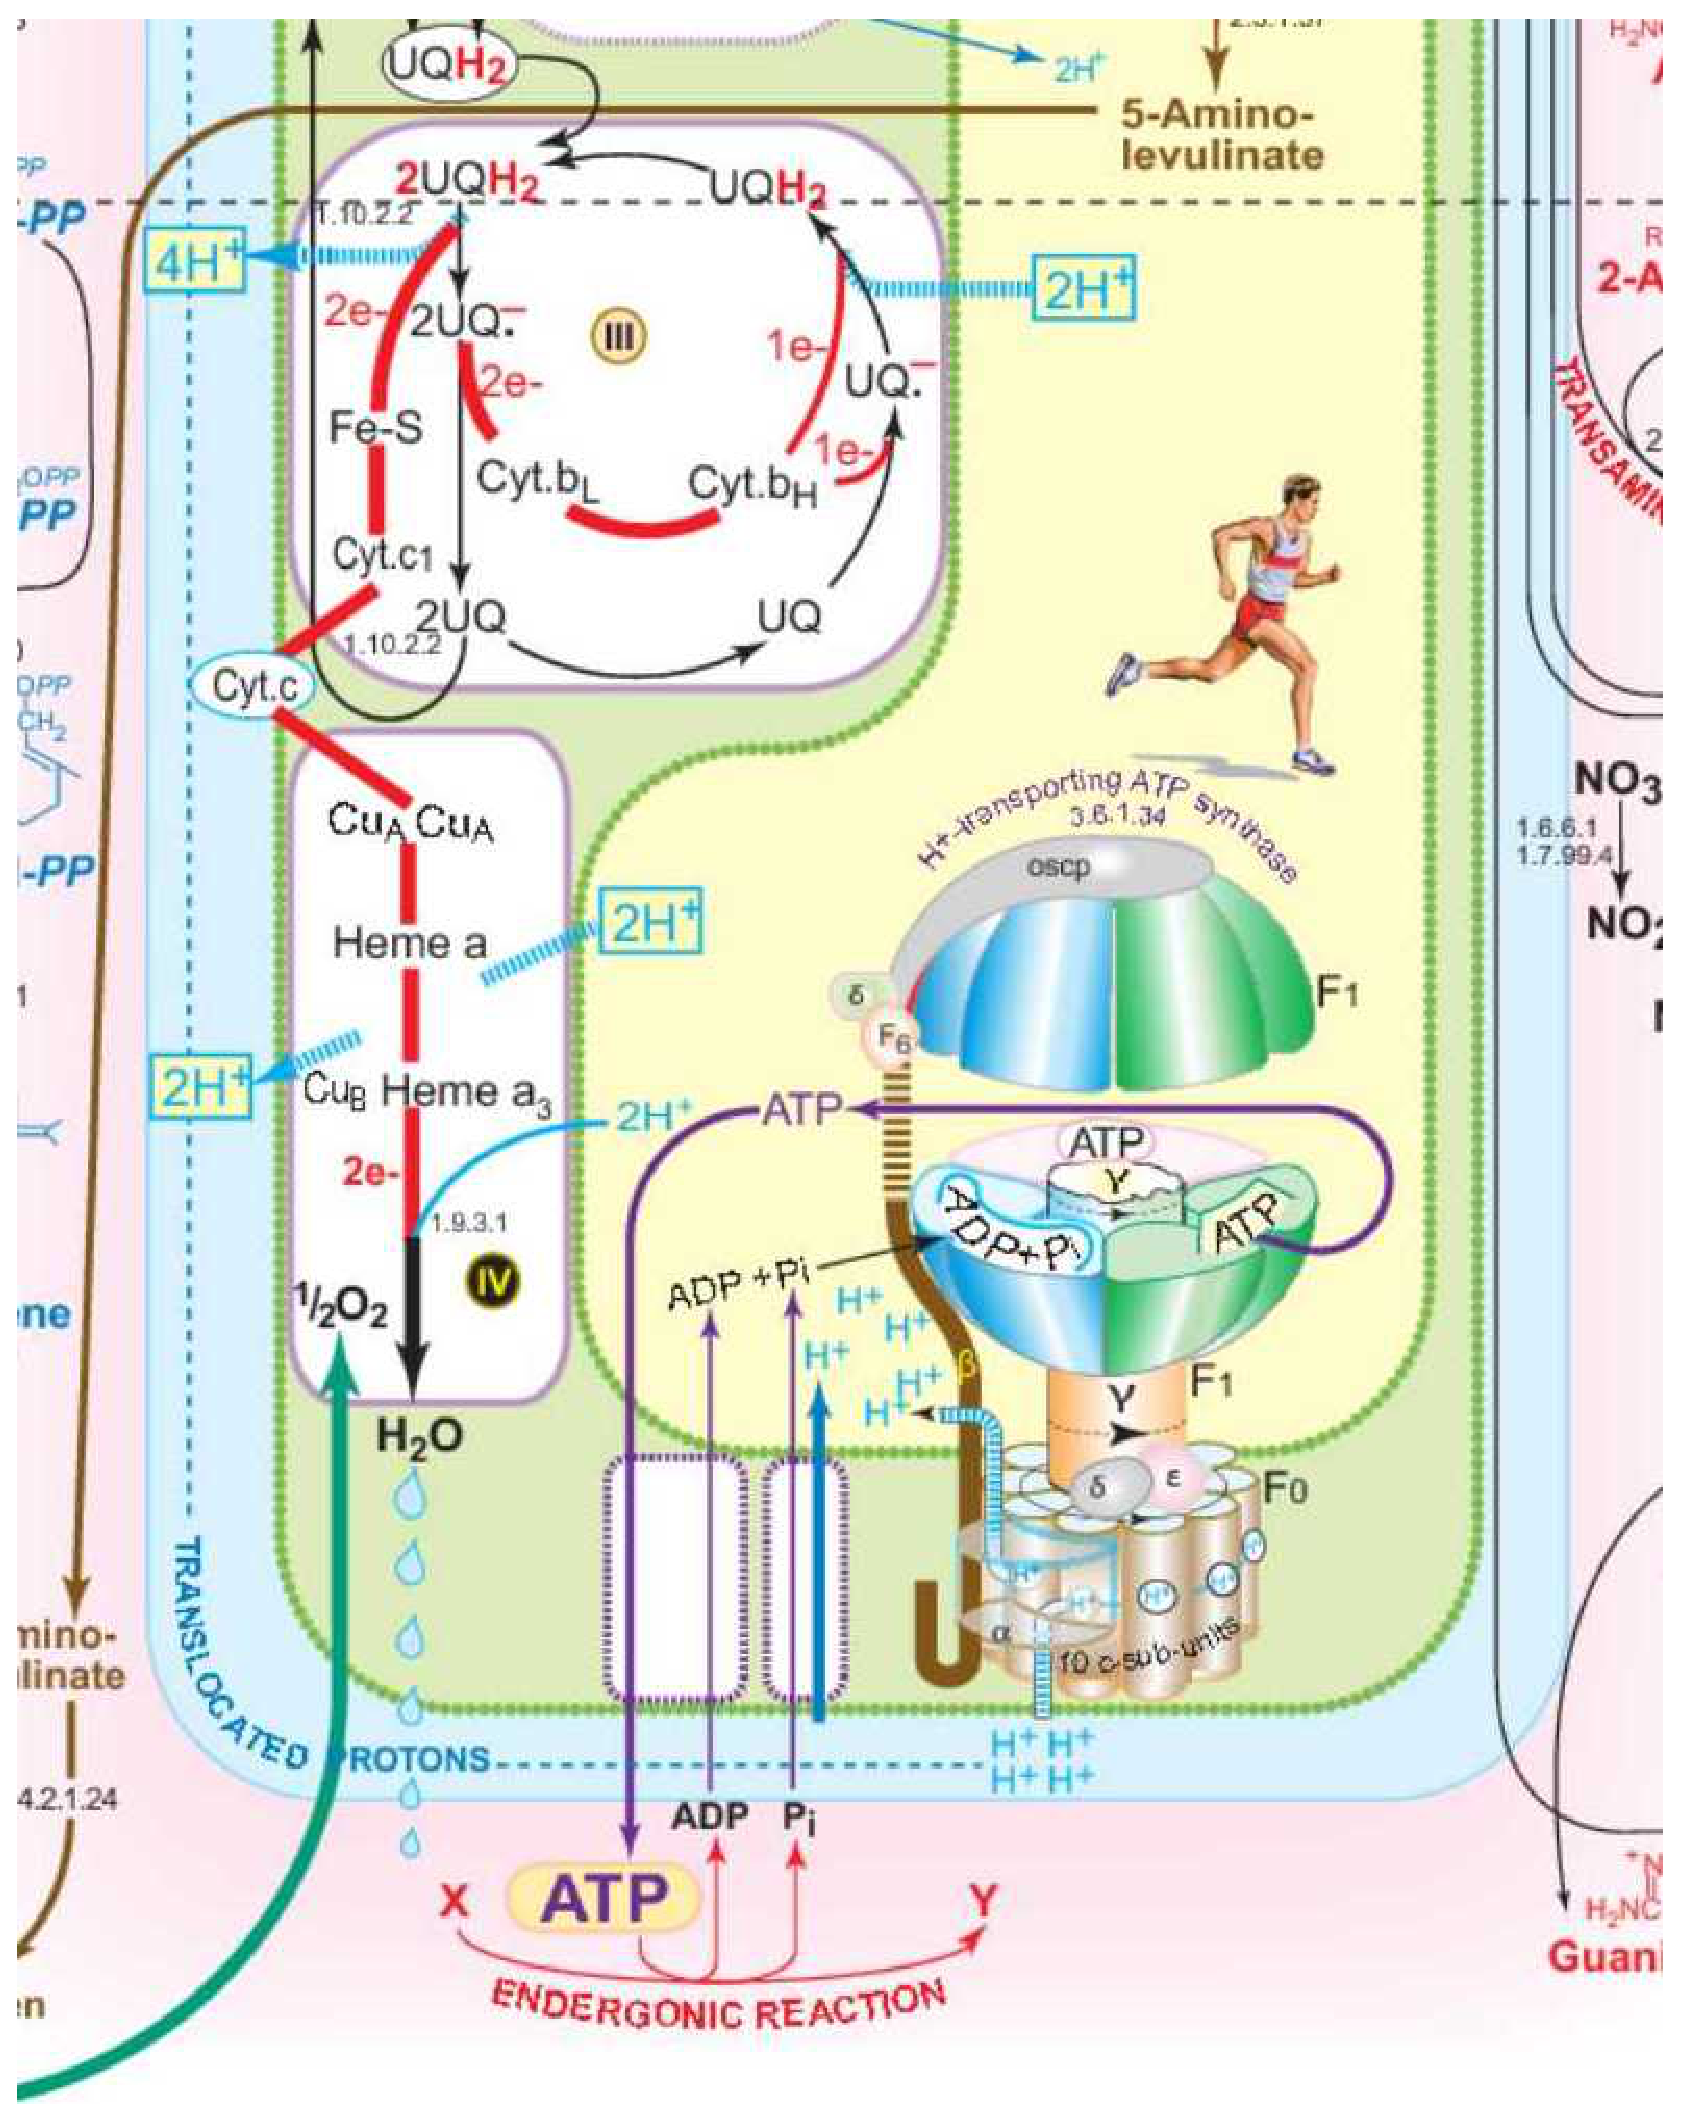
\includegraphics[height=0.85\textheight, width=\textwidth]
{metabolism-zoom-start}
%height=0.85\textheight,width=0.53\textwidth
\end{column}
\begin{column}{0.45\textwidth}
\introduceFlux
\end{column}
\end{columns}
}


\note{\scriptsize
Metabolism can be described as the set of reactions and the rate
of the reactions made possible by enzymatic catalysts.  The rate of a
reaction is called flux, and if we think of the reactions as being roads, 
then the flux of a reaction is the throughput of traffic on the road. 
Enzymes, which are protein catalysts, can be thought of as the width
or the number of lanes of the road.
\par

Metabolism is critical for understanding wide classes of
diseases including diabetes, cancer, and inborn errors in metabolism.
Here we can see several very important reactions that organisms from
yeasts to humans require, the ultimate step being the generation of
ATP by this motor-like enzyme complex called ATP Synthase. We'll come
back to ATP synthase in a later example.
\par

Unfortunately, metabolism is much more complex than is often
depicted, and so the problem of determining fluxes that might help
us to better understand disease is also a difficult problem.
This depiction only shows a little over half of what would
be considered a fairly typical length for a pathway, which is
itself dependent on many pathways of about the same size.
When we zoom out, we can start to see some of
this complexity. 
\par}


\frame{\frametitle{\introduceFluxTitle}
\begin{columns}
\begin{column}{0.55\textwidth}
\includemedia[
  activate=pageopen,
  height=0.85\textheight,
  width=\textwidth,
  transparent=true
]
{}{\commonDir figuresFalconTalk/metabolism-zoom.swf}
\end{column}
\begin{column}{0.45\textwidth}
\introduceFlux
\end{column}
\end{columns}
}

\note{
Here you can see the rest of the first pathway, oxidative
phosphorylation, and its sister pathway, the TCA cycle. And this
little linear pathway is glycolysis, which converts glucose into a
usable form for the TCA cycle. In practice, these pathways also
require many other pathway dependencies that process or recycle other
chemicals that are not quite in the right form to be used by the later
stages. What's more, this poster from 2003 is actually relatively
simple: chemicals that are similar are often omitted, and there can be
thousands of these for some types of chemicals. Also, reactions
thought to be unimportant often are not drawn.
\par

\textbf{Due to all this complexity and the inability to measure most fluxes
directly, as well as the need to quantitatively understand
what the reaction fluxes are, a mechanistic modeling framework is
needed to really get at the system.}
\par}


%%%%%%%%%%%%%%%%%%%%%%%%%%%%%%%%%%%%%%%%%%%%%%%%%%%%%%%%%%%%%%%%%%%%%%%%%%%%%%%%%%%%%%%%%%

\newsavebox{\hideLetter}
\savebox{\hideLetter}{%
{\colorbox{white}{\makebox(0.015\textwidth, 0.03\textheight)[lt]{ }}}%
}

\newsavebox{\toynet}
\newsavebox{\toySmat}
\newsavebox{\FBAeqns}
\newsavebox{\FBAgeom}
\newsavebox{\WIREsCite}

\frame{\frametitle{An overview of constraint-based modeling}

\savebox{\toynet}{%
\includegraphics<1->[width=0.6\textwidth, viewport=0 418 708 718, clip=true]
{SmatExample}}


\savebox{\toySmat}{%
\includegraphics<2->[width=0.6\textwidth, viewport=0 0 708 418, clip=true]
{SmatExample}}


\savebox{\FBAeqns}{%
\includegraphics<3->[width=0.4\textwidth, viewport=411 793 643 938, clip=true]
{SmatExample}}

\savebox{\FBAgeom}{%
\includegraphics<4->[width=0.4\textwidth, viewport=0 712 516 1130, clip=true]
{SmatExample}}

\savebox{\WIREsCite}{\scriptsize%
\hspace{-0.6cm}\textit{Shestov, Barker, Gu, and Locasale. WIREs Syst Biol Med, 2013.}}

% % % %

\begin{picture}(\textwidth, \textheight)
\put(0, \textheight){\makebox(0.5\textwidth, 0)[lt]{\usebox{\toynet}}}
\put(0, 0.95\textheight){\usebox{\hideLetter}}

\put(0, 0.6\textheight){\makebox(0.5\textwidth, 0)[lt]{\usebox{\toySmat}}}
\put(0, 0.555\textheight){\usebox{\hideLetter}}

\put(0.65\textwidth, \textheight){\makebox(0.5\textwidth, 0)[lt]{\usebox{\FBAeqns}}}

\put(0.65\textwidth, 0.6\textheight){\makebox(0.5\textwidth, 0)[lt]{\usebox{\FBAgeom}}}
\put(0.65\textwidth, 0.555\textheight){\usebox{\hideLetter}}
\put(0.98\textwidth, 0.31\textheight){% cover cutoff equations
  \colorbox{white}{\makebox(0.07\textwidth, 0.11\textheight)[lt]{ }}}
\put(0.77\textwidth, 0.55\textheight){% cover 'FBA'
  \colorbox{white}{\makebox(0.07\textwidth, 0.05\textheight)[lt]{ }}}

\put(0, 0.1\textheight){\usebox{\WIREsCite}}


\end{picture}
} % end of \frame


\note{\tiny
To illustrate the modeling concepts that I'll be discussing, let
me briefly introduce a much simpler toy network. Note that the 
network has several chemical reactions, the $F_i$, as well as
transport reactions. Some reactions are drawn
with arrows in both directions and are called reversible reactions.
The distinction between irreversible and reversible is highly
important in our modeling considerations, and we'll be discussing
reversibility more later.
\par

To work with a system computationally, we write all known
reactions down, including transport reactions across compartments, as
the columns of a matrix, called the Stoichiometric matrix or the S matrix.
The rows correspond to compartmentally unique chemicals, often called
metabolites. The entries of the matrix
correspond to the coefficients in the reaction equation: a negative
coefficient denotes it is a reactant, and a positive coefficient
signifies it is a product. For instance, reaction $F_1$ consumes two
$I$ and one $J$ to produce an $A$. 
\par

Now that we have this matrix, we can make mathematical
assumptions about the system. The S matrix multiplied by the flux
vector (here denotes as an $F$, and sometimes as a $\mathbf{v}$)
yields the change in concentration over time for each
metabolite, which is typically constrained to be zero and is called
the steady state assumption. The steady state assumption 
asserts that concentrations do not change over large enough timescales.
Finally, we need an optimization objective. 
\textbf{An objective has a dual meaning: it is
something that we suppose instills the biological imperative of
the cell, and it is a mathematical function that we can optimize.
A common example is the maximization of growth rate, which
is used for many microbes that often grow as fast as the
nutrient supply and physiological constraints will allow.}
The constraints define a feasible region, shown here, and the
optimization objective allows us to find a particular solution, or at
least greatly narrow down the possibilities.
\par

While this framework is powerful, it is also theoretically simplistic
(so far we only make use of a simple objective and the known
reactions). It can also be inaccurate, especially for multicellular
organisms with many different types of cells, where one objective
doesn't fit all.  But the framework is extendable, and in this work,
we augment it by using two types of data: annotation on how the
enzymatic complexes come together, and data on abundance of the
components of these enzyme complexes.
\par}

%%%%%%%%%%%%%%%%%%%%%%%%%%%%%%%%%%%%%%%%%%%%%%%%%%%%%%%%%%%%%%%%%%%%%%%%%%%%%%%%%%%%%%%%%%

\frame{\frametitle{Epistasis} 

\begin{columns}[t]
%
\begin{column}{0.5\textwidth}
\hfill\ul{\textbf{Model}}\hfill
\begin{itemize}
\item \textit{Genetic interactions}
\item Genes X and Y
\item Fitnesses relative to wild-type
\item Single mutant fitnesses $W_x$ and $W_y$
\item Double mutant fitness $W_{xy}$
\item $\epsilon = W_{xy} $ -- $W_xW_y$   %not sure why $-$ isn't rendered
\end{itemize}
\end{column}

\begin{column}{0.5\textwidth}
\hfill\ul{\textbf{Applications}}\hfill
\begin{itemize}
\item Evolution of sex
\item Speciation
\item Mutational load
\item Ploidy
\item Genetic drift
\item Drug interactions \& disease
\item Complex traits
\end{itemize}
\end{column}

%
\end{columns}
} % end of \frame


%%%%%%%%%%%%%%%%%%%%%%%%%%%%%%%%%%%%%%%%%%%%%%%%%%%%%%%%%%%%%%%%%%%%%%%%%%%%%%%%%%%%%%%%%

\frame{\frametitle{Flux restrictions in two reactions can cause sign-epistasis}

\begin{figure}
\centering
\includegraphics[height=0.8\textheight]{Figure_S2}
\end{figure}
}

%%%%%%%%%%%%%%%%%%%%%%%%%%%%%%%%%%%%%%%%%%%%%%%%%%%%%%%%%%%%%%%%%%%%%%%%%%%%%%%%%%%%%%%%%

\frame{\frametitle{Increasing flux restriction increases the
percentage of negative epistasic interactions.}

\begin{figure}
\centering
  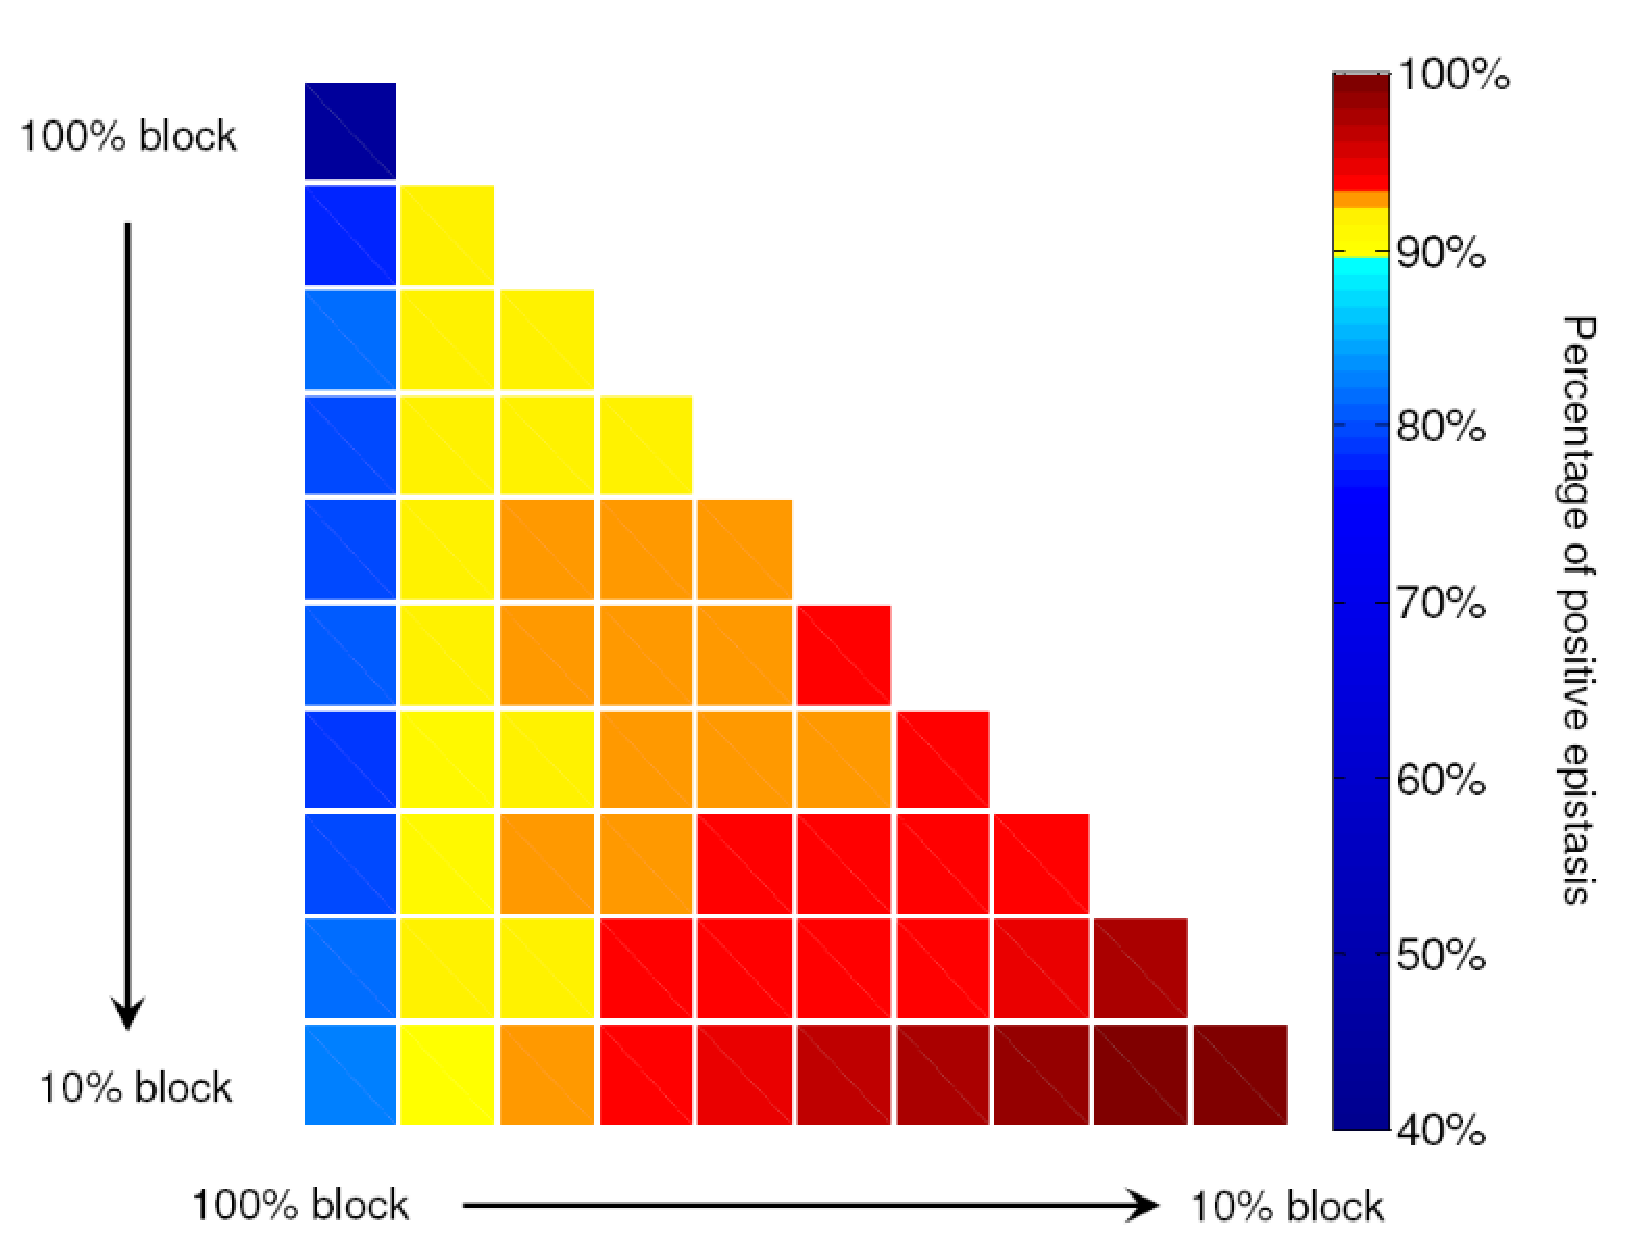
\includegraphics[height=0.75\textheight]{deleteriousYeastEpiLandscape}
\end{figure}
}

%%%%%%%%%%%%%%%%%%%%%%%%%%%%%%%%%%%%%%%%%%%%%%%%%%%%%%%%%%%%%%%%%%%%%%%%%%%%%%%%%%%%%%%%%

\frame{\frametitle{Epistatic relations between genes are allele specific} 

\begin{figure}
\centering
  \includegraphics[height=0.7\textheight, viewport=16 370 395 618, clip=true]
  {sgeFigure_1}
\caption{Results based on FBA simulations. Solid and broken lines
represent mean and 95\% confidence intervals, respectively.}
\label{fig:FBAdynEpi}
\end{figure}
}

%%%%%%%%%%%%%%%%%%%%%%%%%%%%%%%%%%%%%%%%%%%%%%%%%%%%%%%%%%%%%%%%%%%%%%%%%%%%%%%%%%%%%%%%%%

\frame{\frametitle{Epistatic relations between genes are allele specific} 

\begin{figure}
\centering
  \includegraphics[height=0.65\textheight, viewport=20 16 398 273, clip=true]
  {sgeFigure_1}
\caption{Cumulative distribution for the percentage of shared
epistatic interaction partners between two mutant alleles 
on real experimental data. Broken lines represent
10\% and 20\% of shared epistatic profiling.}
\label{fig:ExpdynEpi}
\end{figure}
}

%%%%%%%%%%%%%%%%%%%%%%%%%%%%%%%%%%%%%%%%%%%%%%%%%%%%%%%%%%%%%%%%%%%%%%%%%%%%%%%%%%%%%%%%%%


\frame{\frametitle{Mutant alleles in the same gene with more severe defects tend
to have a higher percentage of negative epistasis in yeast.} 

\begin{figure}
\centering
  \includegraphics[height=0.65\textheight, viewport=48 421 479 682, clip=true]
  {sgeFigure_2}
\label{fig:ExpFBAconfirm:A}
\end{figure}
}

%%%%%%%%%%%%%%%%%%%%%%%%%%%%%%%%%%%%%%%%%%%%%%%%%%%%%%%%%%%%%%%%%%%%%%%%%%%%%%%%%%%%%%%%%%

\frame{\frametitle{Eukaryotic models tend to exhibit prevalent negative epistasis in
severe mutants.} 

\begin{figure}
\centering
  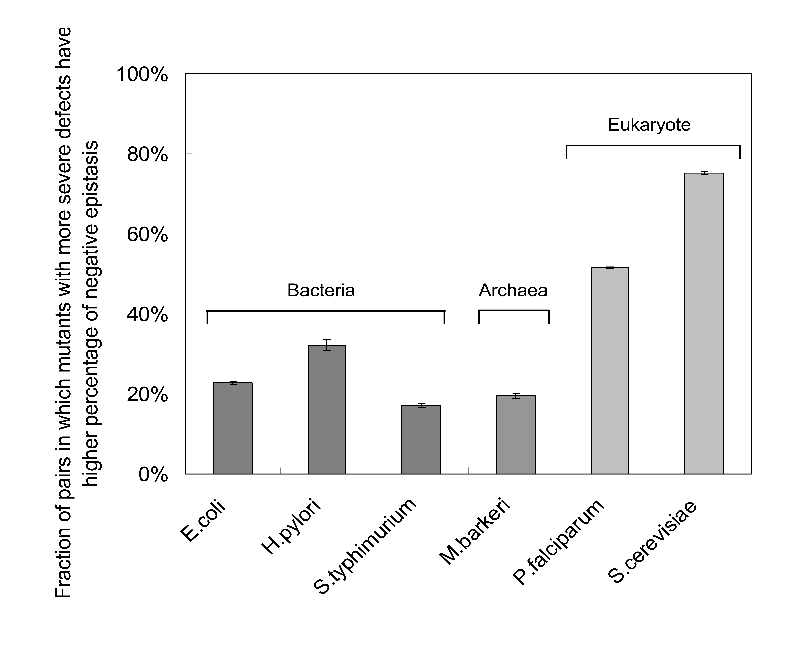
\includegraphics[height=0.8\textheight]
  {sgeFigure_3}
\label{fig:ExpFBAconfirm:A}
\end{figure}
}

%%%%%%%%%%%%%%%%%%%%%%%%%%%%%%%%%%%%%%%%%%%%%%%%%%%%%%%%%%%%%%%%%%%%%%%%%%%%%%%%%%%%%%%%%%

\frame{\frametitle{An objective for fitting fluxes}
\begin{block}{Find the best detour due to road construction}
Started as a way to fit a perturbed model to an original flux.\\
\vspace{1ex}
Can also be used to fit empirical flux estimations in a model.\\ 
\vspace{1ex}
Formulated as quadratic least-squares optimization\\(Segr\`e et al 2002):\\
\begin{center}
$\textnormal{minimize}\ \sum\limits_{i=1}^N (v_i-a_i)^2$ 
\end{center}
Later formulated as a linear programming (LP) variant.
% \vspace{1ex}\hrule\vspace{1ex}
% \textit{find the best detour due to road construction}
\end{block}

\begin{block}{Fitting fluxes from expression is more difficult}
But important: expression tells us what the system can do.\\
\vspace{1ex}
Flux tells us what the system is doing.
\end{block}
}

\note{\scriptsize
Having discussed one type of biological objective, let's move to a
type of objective that relates directly to our present study, that of
flux fitting. \textbf{Flux fitting can be thought of in terms of our
road analogy as a traffic jam or construction work causing a
detour. We want the detour to be as short as possible while getting us
to our original destination, and not disrupting traffic elsewhere.}
\par

In actuality, this is very similar to the first application of flux fitting, 
which was to mutate a model by knocking out certain reactions to see what the
mutant phenotype would be, with the original flux, here denoted by the
$a_i$ found by some other objective, such as the aforementioned growth
rate maximization. The same objective can be used to estimate a global
flux fit for the model when we only know some of the $a_i$ from
experimental measurements. Mathematically the objective is just a
constrained least squares problem, which also has a linear variant
that makes it amenable to linear programming solvers.  In our work, we
also use the linear programming variant.
\par

Fitting fluxes to expression, rather than to other fluxes, is more
difficult.  This is a mathematical issue that arises from the fact
that expression is non-negative but fluxes are bidirectional and can
assume any real value. \textbf{ Despite this difficulty, it is
important to develop efficient methods for calculating the flux from
expression due to the abundance of medically important expression
data, since expression only tells us what the cell is capable of doing
and flux tells us what the cell is, in fact, doing.}
\par}

%%%%%%%%%%%%%%%%%%%%%%%%%%%%%%%%%%%%%%%%%%%%%%%%%%%%%%%%%%%%%%%%%%%%%%%%%%%%%%%%%%%%%%%%%%

\frame{\frametitle{From expression to enzyme complex abundance}

% \begin{block}{Expression-flux fitting}
% Expression is widely available, especially for diseases. \\
% \vspace{1ex}
% But, expression must be converted to enzyme abundance. 
% \end{block}
\hspace*{0.12\textwidth}(genes)\hspace*{0.09\textwidth}(``expression'')%
\hspace*{0.05\textwidth}(``protein expression'')
\begin{figure}
\centering
%\begin{tabular}{cc}
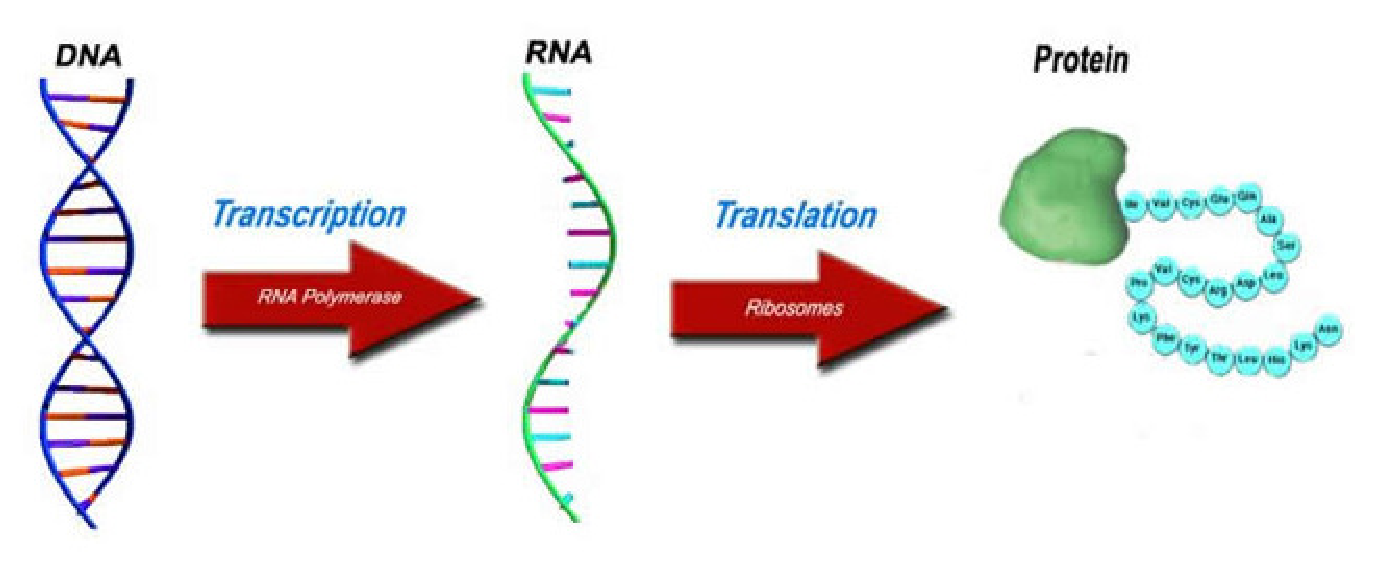
\includegraphics[width=0.7\textwidth]{centraldogma} \\ % 
%& %
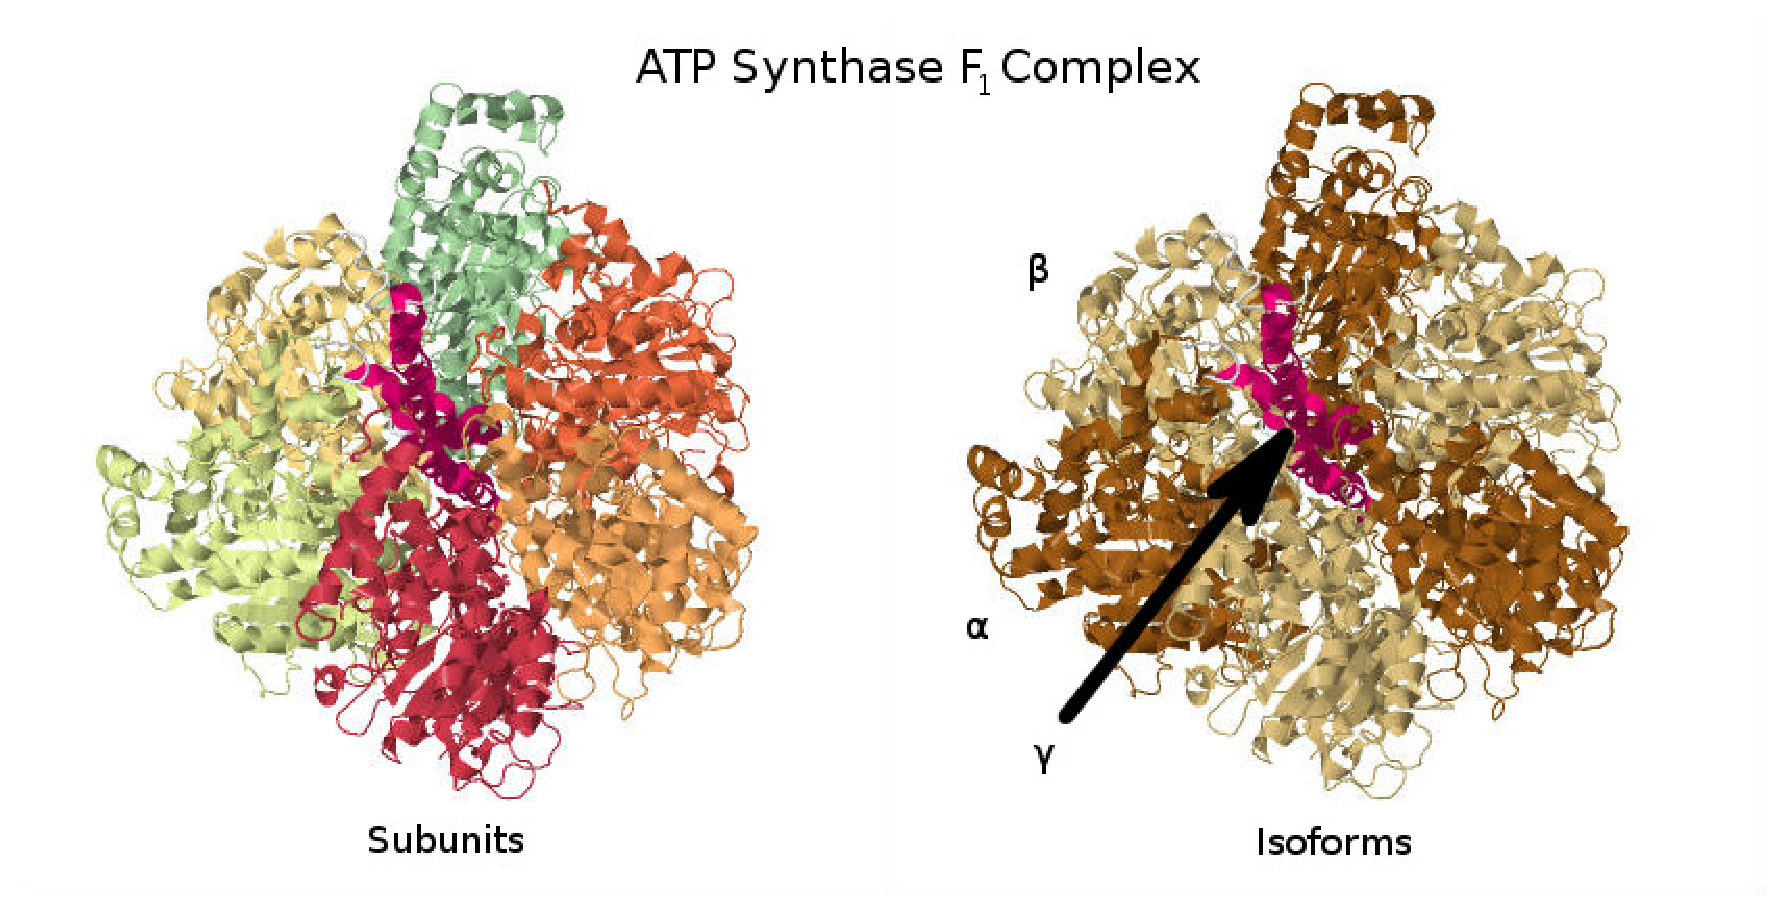
\includegraphics[width=0.7\textwidth]{2F43} %
%\end{tabular}
\end{figure}
}

\note{\scriptsize
Before we get into the details of estimating flux from expression, it
is helpful to know how enzyme complexes are formed, as these are the
fundamental catalytic units for biological reactions. Genes are
encoded in DNA, which can be thought of as the master blue prints.
Copies of these blue prints are made, and are sent out to be converted
into proteins. Since reading a template and building a protein takes
time, the the number of these RNA template copies roughly
correlates with the amount of protein created. Quantities of both RNAs
and proteins can be called expression, but typically we use it to
refer to the former, since measurement of RNA is far easier
experimentally. Though still no walk in the park, RNA measurement 
has become widely used due to low cost.
\par

Once we have the proteins, it is often the case that a single protein
is not catalytic on its own, and must join with other proteins in
order to be functional. Here is a visualization of a famous protein
subcomplex that we saw earlier, part of ATP synthase.  This protein
has 7 individual protein molecules, called subunits. But in total,
there are only three genes that contribute to this subcomplex.  The
expression of each of these genes is what we have to go on when trying
to quantify the overall complex, along with which genes are a part of
the complex and whether or not their function within the complex can
be assumed by some other gene. 
\par}

%%%%%%%%%%%%%%%%%%%%%%%%%%%%%%%%%%%%%%%%%%%%%%%%%%%%%%%%%%%%%%%%%%%%%%%%%%%%%%%%%%%%%%%%%%

\frame{\frametitle{Boolean gene rules can help quantify enzyme complexes}

\begin{block}{Equivalent gene rules can be evaluated differently}
For genes A, B, and C:\\
Rules $r_1$ and $r_2$ are equivalent logically.\\
However, they can be interpreted differently.
\end{block}

\begin{center}
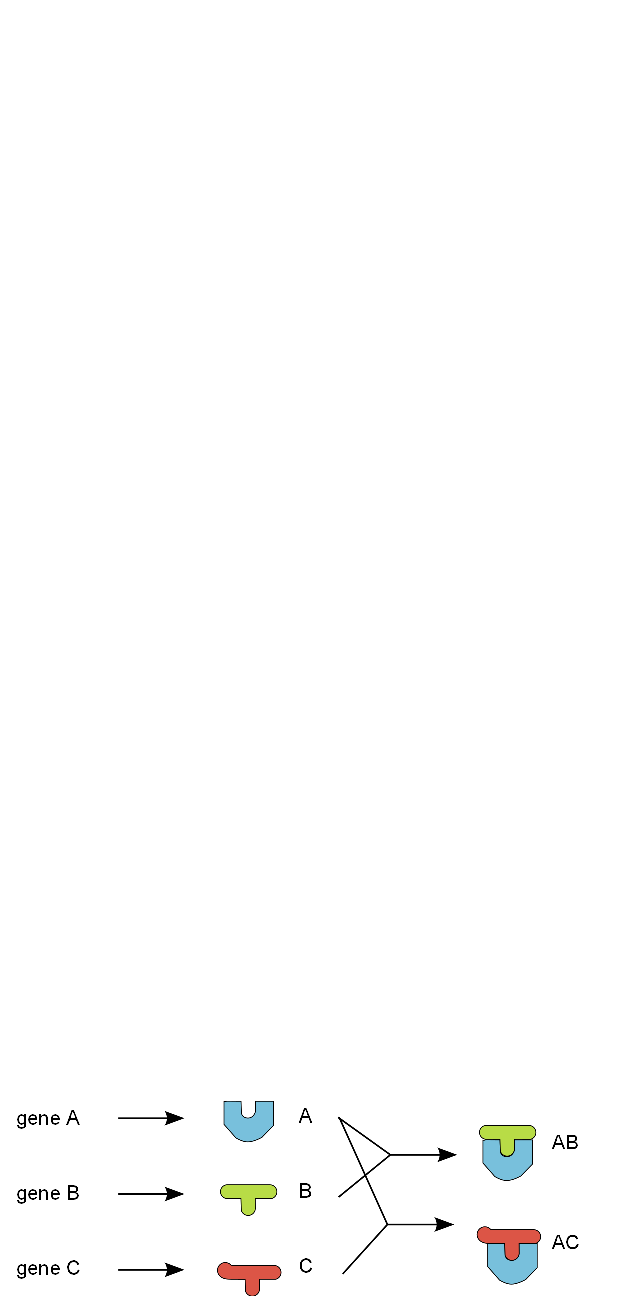
\includegraphics[width=0.8\textwidth]{GPRrules_diagram}
\vspace{1ex}
\begin{tabular}{cccccccc}
$r_1$ & := & [A and B] or [A and C] & $\rightarrow$ & $e_1$  &=& $\min(a,b$) + $\min(a,c$) \\ 
$r_2$ & := & [A and (B or C)]       & $\rightarrow$ & $e_2$  &=&  $\min(a, b + c$) 
\end{tabular} 
\end{center}
}

\note{\scriptsize
\textbf{This relationship between necessity or redundancy of a gene in a
complex is annotated in models as Boolean gene rules.} Previously, a
study from a collaborator noted that one possible way of doing
quantification is to substitute the gene names with the expression
levels, the ANDs with minimums, and the ORs with sums. This is great
intuition since an AND rule states that both genes are required, so
the minimum amount of either gene will limit the formation of the
complex, and an OR rule similarly states that there is redundancy of
the genes within the complex, so that the expression of both genes may
be summed. However, problems frequently arise in practice, as illustrated
in this example. We can look at two simple rules, $r_1$ and $r_2$,
that are logically equivalent, but when evaluated with direct substitution, 
lead to two different results. In the case of $r_1$, the level of $a$ can
is double counted if it is in fact the minimum value of $a$, $b$, and $c$.
\par

This issue does not occur in $r_2$, which has a special structure
known in computer science as conjunctive normal form, where the rule
is a conjunction of many disjunctions, or more plainly, an AND of many
ORs.  A major part of our work has been to show that conjunctive
normal form makes sense in the general case. We call our method for
enzyme complex quantification 'min disjunction', since we are finding
the minimum of all disjunctions.
\par}

%%%%%%%%%%%%%%%%%%%%%%%%%%%%%%%%%%%%%%%%%%%%%%%%%%%%%%%%%%%%%%%%%%%%%%%%%%%%%%%%%%%%%%%%%%

\frame{\frametitle{An example of a larger gene rule in Human Recon 2}

\tiny

%%%%%%%%%%%%%%%%%%%%%%%%%%%%%%%%%%%%
                                   %
\input{\commonDir exampleRule.tex} %
                                   %
%%%%%%%%%%%%%%%%%%%%%%%%%%%%%%%%%%%%
}
\note{
Now that we know the kind of rule we need, we need to write software that
can parse the rues into an abstract syntax tree so they can be
manipulated into conjunctive normal form.  This is the main reason why
we developed a parser for gene rules, instead of just using regular
expression substitution as was done previously. This has another
benefit; some rules can be quite large. There are several examples in
the human model, such as this one, that won't even fit on a page given
a tiny font. In fact, it would take tens of of pages. The reason for
this is due to having alternative proteins fulfilling identical roles
within a large complex. It took many minutes to deal with such a rule
using the original regular expression framework, 
whereas using our framework takes far less than a second.
}% end of \note


%%%%%%%%%%%%%%%%%%%%%%%%%%%%%%%%%%%%%%%%%%%%%%%%%%%%%%%%%%%%%%%%%%%%%%%%%%%%%%%%%%%%%%%%%%

%%%%%%%%%%%%%%%%%%%%%%%%%%%%%%
                             %
\section{Methods \& Results} % 
\subsection{Complexation}    %
                             %
%%%%%%%%%%%%%%%%%%%%%%%%%%%%%%

%%%%%%%%%%%%%%%%%%%%%%%%%%%%%%%%%%%%%%%%%%%%%%%%%%%%%%%%%%%%%%%%%%%%%%%%%%%%%%%%%%%%%%%%%%

\begin{frame}[fragile]
\frametitle{An efficient pipeline going from gene expression to flux}

\begin{columns}
\begin{column}{0.45\textwidth}
\begin{figure}
\centering
\begin{tikzpicture}[scale=0.5, every node/.style={scale=0.5}]%[scale=0.8, node distance = 1cm, auto]
    % Place nodes
    \node [block] (start) {start}; 
    \node [iogram, below of=start, left of=start, xshift=-0.2cm] (exp) {Genes:\\ expression 
      ($\mu$,~$\sigma$)}; 
    \node [iogram, below of=start, right of=start] (rules) {Reactions:
      Gene Rule}; 
    \node [block, below of=rules, onslide=<1>{fill=yellow!80}] (parse) {Parse Rule}; 
    \node [block, below of=parse, left of=parse, xshift=-0.5cm, onslide=<2>{fill=yellow!80}]
      (mindisj) {Find minimum disjunction};
    \node [iogram, below of=mindisj] (expstd)
          {Reactions (enzyme~complexes):\\ abundance ($\mu$,~$\sigma$)};
    \node [iogram, right of=falcon, below of=expstd, xshift=0.2cm] (smat) 
      {$\mathbf{S}$ matrix};
    \node [iogram, left of=falcon, below of=expstd, xshift=-0.3cm] (vbnd) 
      {Reactions:\\ flux bounds ($\mathbf{v}_{lb}$, $\mathbf{v}_{ub}$)};
    \node [block, below of=vbnd, left of=smat, right of=vbnd, 
      below of=expstd, yshift=-0.5cm, onslide=<3>{fill=yellow!80}] (falcon) 
      {Flux fitting (FALCON)};
    \node [iogram, below of=falcon] (fluxout) 
      {Reactions:\\ fluxes ($\mathbf{v}:$ $\mu$,~$\sigma$)};


    % Draw edges
    \path [line] (start) -- (exp);
    \path [line] (start) -- (rules);
    \path [line] (rules) -- (parse);
    \path [line] (exp.south) -- (mindisj);
    \path [line] (parse) -- (mindisj);
    \path [line] (mindisj) -- (expstd);
    \path [line, transform canvas={xshift=0.1cm}] (expstd) -- (falcon);
    \path [line] (rules.east) |- (falcon.east);
    \path [line] (smat) -- (falcon);
    \path [line] (vbnd) -- (falcon);
    \path [line] (falcon) -- (fluxout);
\end{tikzpicture}
\end{figure}
\end{column}

\begin{column}{0.55\textwidth}

{\color{gray!65}

{\only<1>{\color{black}}
\begin{lstlisting}[basicstyle=\ttfamily\tiny, language=ATS, showstringspaces=false]


fun parse_fileref (inp: FILEref): grexplst
fun parse_grexplst (!tokener): grexplst
fun parse_grexp (!tokener): grexp


\end{lstlisting}}

{\only<2>{\color{black}}
\begin{lstlisting}[basicstyle=\ttfamily\tiny, language=ATS, showstringspaces=false]



fun grexplst_cnfize (gxs: grexplst): grcnflst
// Easily done with templates:
implement
grexplst_cnfize (gxs) =
  list_map_fun<grexp><grcnf> (gxs, grexp_cnfize)
//
fun grexp_cnfize (gx: grexp): grcnf
//
fun grcnf_minmean_stdev
  (grcnf: !grcnf, emap: GDMap, smap: GDMap): expvar
\end{lstlisting}}

\vspace{4ex}

{\only<3>{\color{black}}
\begin{lstlisting}[basicstyle=\ttfamily\tiny, language=MATLAB, showstringspaces=false]
function [e, e_sd, rxn_rule_group] = ...
    computeMinDisj(model, genedata_filename)
function v = falcon(model, e, e_sd, varargin)
\end{lstlisting}}

} % end of \color{gray}
\end{column}

\end{columns}

\end{frame}


\note{\tiny
Now we can take a moment to look at the big picture of our flux
estimation framework. On the right side of the screen I've shown the
main interfaces we've used for each part of the processes in the
flowchart; the first two processes are implemented in a StandardML
variant, and the last process, which is the one most users will
be working with, is in MATLAB.
\par

Taking as inputs the gene rules and the mean and standard deviation of
all genes' expression values from a sample, we parse the rule into an
abstract syntax tree, called a grexp, short for gene rule expression. 
Since users may be interested in various levels
of experimentation, the first function, which
parses a list of gene rules found in a file, is implemented in terms
of the second function, which parses a list of gene rules emitted from
a tokenizer. Finally, this function itself is built on the parse\_grexp
function, which parses a single gene rule.
\par

Now we are interested in working with the grexps or grexplsts, and
converting them into conjunctive normal form. We define a new type,
grcnflst, to denote this special form of the grexplst. It is actually
a much simpler type that is essentially a list of list of genes, since
the outer list is taken to be joined by an AND, and the inner lists
joined by ORs. This has the additional benefit of preventing
operations that should only be performed on rules in conjunctive normal form
from being performed on more general rules. This function, which returns a
list of cnfized rules, can be easily implemented in the language by
using a template function, list\_map\_fun, with the corresponding
function grexp\_cnfize which converts a single rule to conjunctive
normal form. Finally we have a function that takes a map of gene names
to values (actually one each for the mean and standard deviation of
expression), and returns a tuple type with the mean and standard
deviation of the complex.
\par

The flux fitting algorithm and interface are implemented in MATLAB.
The first function shown is just a MATLAB interface to the last
function shown above it, with the additional
functionality of identifying which reactions belong to a specific
enzyme complex, which we'll discuss more soon. The return values
of computeMinDisj are inputs to falcon, which will estimate a flux
vector.
\par

Although I haven't shown nearly all of the functions used in our
framework, these are the main functions and give a taste of how the
system can be used.  If we have time, I can show a couple of examples
of these functions being used.
\par}

%%%%%%%%%%%%%%%%%%%%%%%%%%%%%%%%%%%%%%%%%%%%%%%%%%%%%%%%%%%%%%%%%%%%%%%%%%%%%%%%%%%%%%%%%%

\frame{\frametitle{Method comparison for enzyme complex quantification}
\framesubtitle{The effect on FALCON-estimated fluxes} 

\begin{figure}
\centering
\begin{tabular}{cc}
  \begin{subfigure}[b]{0.5\textwidth}
  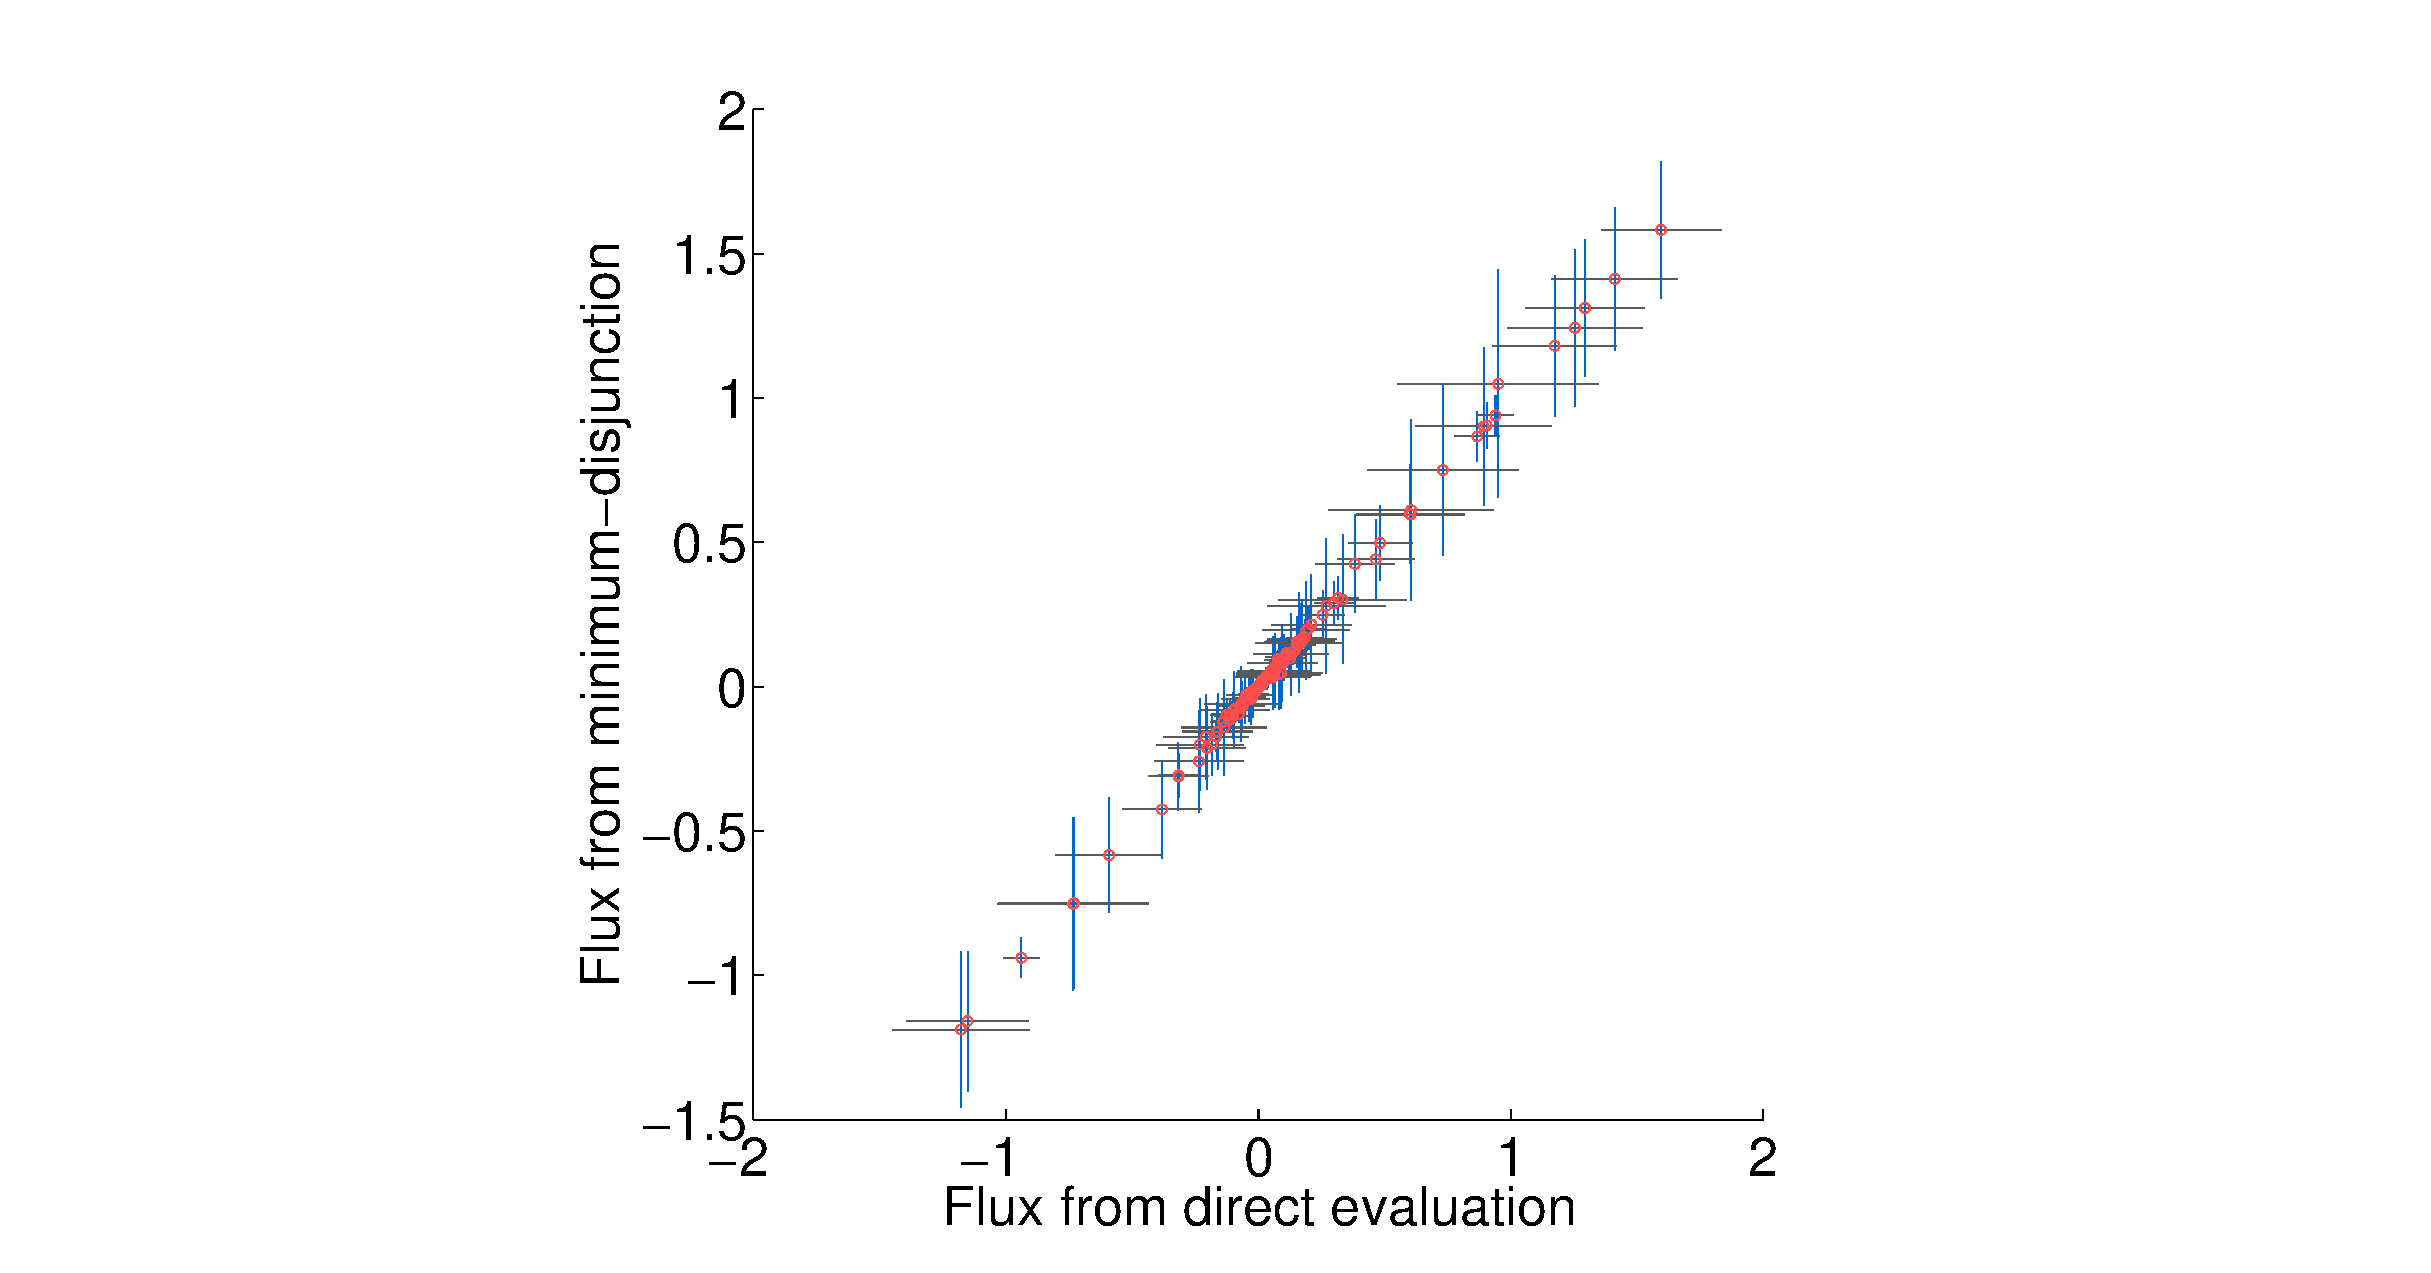
\includegraphics[width=\textwidth, trim=9cm 0cm 9cm 0cm, clip=true]
  {expCmpY7MC}
  \caption{yeast} \label{fig:EnzAbundEval:B}
  \end{subfigure} 
&
  \begin{subfigure}[b]{0.5\textwidth}
  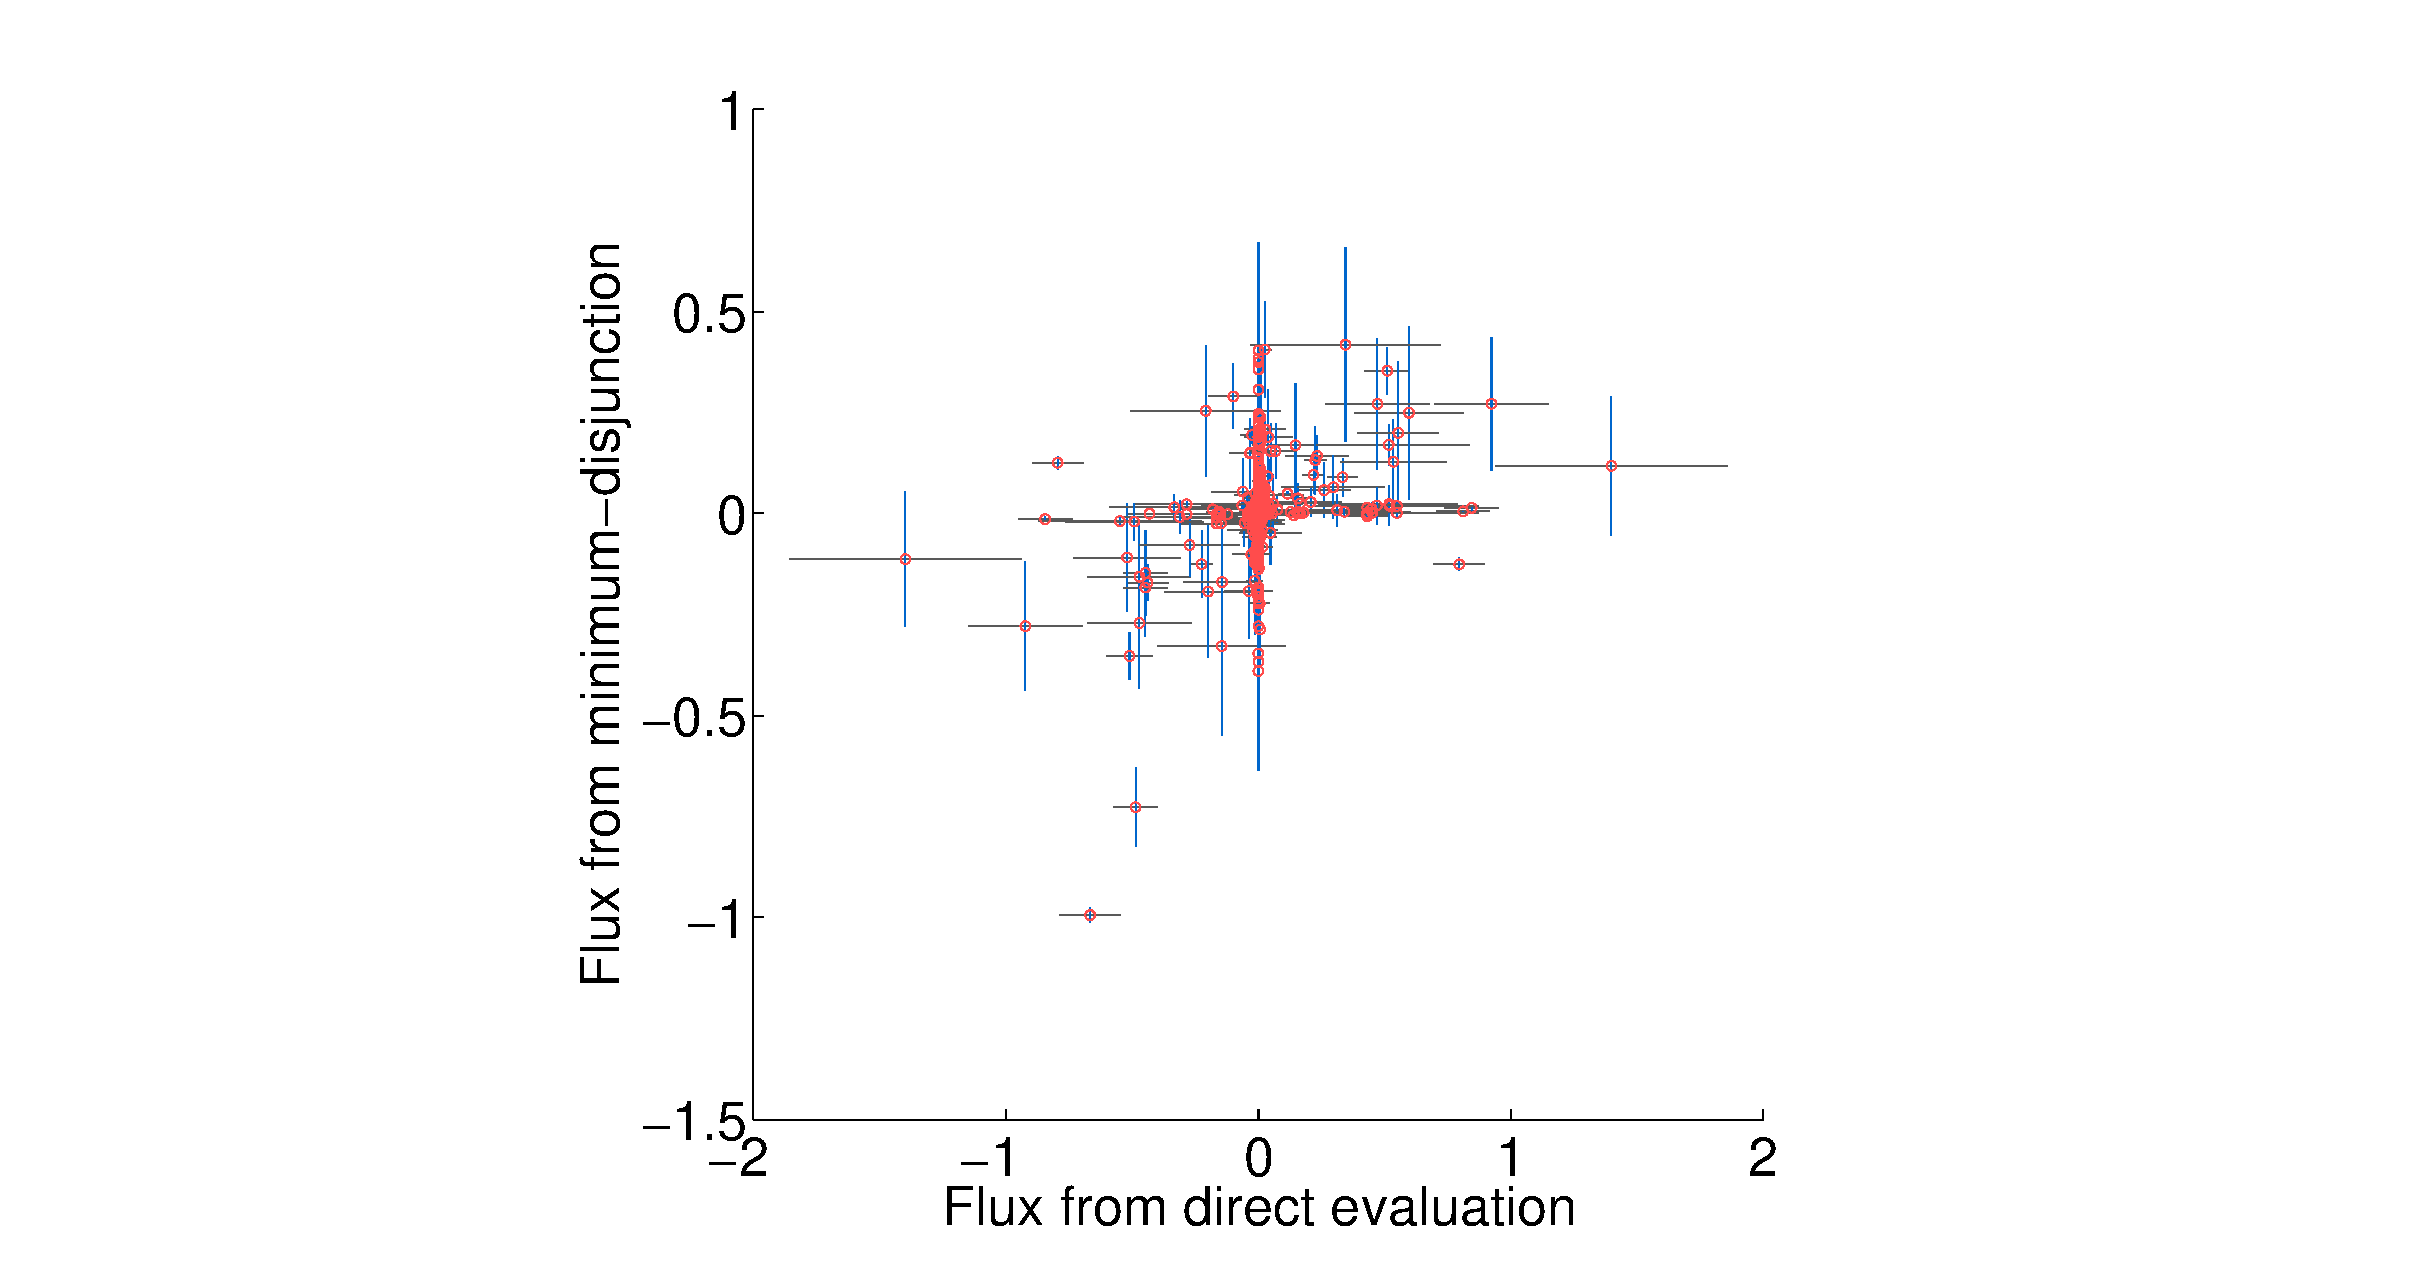
\includegraphics[width=\textwidth, trim=9cm 0cm 9cm 0cm, clip=true]
  {expCmpR2dC}
  \caption{human} \label{fig:EnzAbundEval:D}
  \end{subfigure} 
\\
\end{tabular}
\vspace{-4mm}
\label{fig:EnzAbundEval}
\end{figure}
}

\note{
A first application of our entire framework can be to see what effect
the first part of our framework, enzyme complex quantification, will
have when substituted with the previously used direct evaluation
method.  The x axis of both figures shows flux values when
calculated from direct evaluation, and the y-axis from our minimum
disjunction method.  We can see that there is relatively little effect
for yeast, which has simple rules compared to the human model, where
the difference between rules can have a much larger effect.
\par}

%%%%%%%%%%%%%%%%%%%%%%%%%%%%%%%%%%%%%%%%%%%%%%%%%%%%%%%%%%%%%%%%%%%%%%%%%%%%%%%%%%%%%%%%%%

\begin{frame}[fragile]
\frametitle{An overview of the FALCON flux-fitting algorithm}

\begin{figure}
\centering
\begin{tikzpicture}[scale=0.5, every node/.style={scale=0.5, font=\Large}]
%[scale=0.8, node distance = 1cm, auto]

\node [iogram] (start) 
  {enzyme abundance ($e_i$),\\ 
  model ($\mathbf{S}$ matrix, $\mathbf{v}_{lb}$, $\mathbf{v}_{ub}$)}; 


\node [block, right of=start, xshift=6.5cm] (LFP) 
  {Call LP solver:\\  minimize $\sum\limits_i \left|\left|v_i\right| -n e_i\right|$ 
  \\ (for all irreversible reactions)};

\node [block, right of=LFP, xshift=6.5cm] (assign_dir) 
  {For all reactions, if:\\
  $v_{f} + v_{b} > 0, v_{f} \neq v_{b}$ \\
  then constrain the smaller of \\
  $v_{f}$ and $v_{b}$ to be $0$.};

\node[align=center,draw, fill, gray!25, text=black, cloud
  callout,cloud puffs=17,cloud puff arc =190,callout pointer
  segments=2, above of=assign_dir, xshift=-1cm, yshift=3.8cm,
  aspect=4,scale=1, inner sep=-25pt] (roadFALCON) 
  {We only care about non-zero net traffic,\\
   not the total traffic in both directions.};

\node [decision, below of=LFP, yshift=-2.5cm, aspect=2] (if_irrev_inc) 
  {If the number of\\ irreversible reactions increased};

\node [iogram, left of=if_irrev_inc, xshift=-6cm] (Vout) {$\mathbf{v}$};


\path [line] (start) -- (LFP);
\path [line] (LFP) -- (assign_dir);
\path [line] (assign_dir) -- (if_irrev_inc);
\path [line] (if_irrev_inc) -- node [midway,above] {\color{black} No} (Vout) ;
\path [line] (if_irrev_inc) -- node [midway,right] {\color{black} Yes} (LFP) ;

\end{tikzpicture}
\end{figure}

\end{frame}

\note{\tiny
Now that we've discussed the gene rule effects in detail, I'd like
to focus on the flux fitting algorithm and some of the improvements we've
made over the initial formulation. 

The intuition for the algorithm is that, if more enzyme is available,
then more flux can flow through the reaction. In addition, it is
unlikely that the organism will highly overproduce enzymes relative to
the flux demands, as this would be extremely wasteful energetically
and in terms of cellular space. Therefore, we wish to minimize the
difference between the absolute value of the flux and the enzyme
abundance, assuming the units have been scaled.
\par

First we call the linear programming solver to minimize the difference
between flux and scaled expression on a non-empty set of irreversible
reactions.  The objective shown is a simplified formulation of the
problem; the presence of absolute values and the scaling constant $n$
requires a transformation of the problem into a linear fractional
program, which can subsequently be transformed into an equivalent
linear programming problem. After this step, we
want to assign reaction directionality whenever there is a preference
for the forward or backward reaction. It is helpful to break down
the original flux, which can be positive or negative, into a forward
and backward flux, $v_f$ and $v_b$, that can only be non-negative.
\textbf{This can be thought of in terms of our road analogy again: we aren't
interested in the total amount of traffic in opposing lanes, but only
the net flow of traffic, so we can see which side of the highways we
want to build our gas stations on.  I promise, that'll be the last
time I use the road analogy.} If there is a preference in direction,
we assigning the other direction to be zero.
\par

If the number of irreversible reactions increased, then we repeat the
process, as the constraints on the system have been updated. 
But if nothing changed since the last time, nothing will
ever change, so we terminate the process and return the flux vector.
\par}

%%%%%%%%%%%%%%%%%%%%%%%%%%%%%%%%%%%%%%%%%%%%%%%%%%%%%%%%%%%%%%%%%%%%%%%%%%%%%%%%%%%%%%%%%%

\frame{\frametitle{Novel features in FALCON flux-fitting}

{%
\setbeamercolor{local structure}{fg=CUGrey}
\setbeamercolor{itemize/enumerate body}{fg=gray!65}
\setbeamertemplate{alerted text begin}{%
  \setbeamercolor{local structure}{fg=CURed}%
  \setbeamercolor{alerted text}{fg=black}%
  }
\begin{itemize}
  \alert<1>{
  \item Automatic expression scaling
    \begin{itemize}
      \footnotesize
      \item Expression scaling 'constant' is now a variable in the L(F)P
      \item Introduces less bias in a scaling constant
    \end{itemize}
  } % end of \only<1>
  \alert<2>{
  \item Grouping reactions by enzyme complex:\\
    $\left|\sum\nolimits_{j \in R_i} (v_{j,f} + v_{j,b}) - n e_i\right|$
    \begin{itemize}
      \footnotesize
      \item Much more principled approach
      \item Major difference for some reactions\\
            ($>$60 reactions per group in some cases)
    \end{itemize}
  } % end of \only<2>
  \alert<3>{
  \item Batch evaluation of reaction directionality
    \begin{itemize}
      \footnotesize
      \item Primary reason for increased speed
      \item Introduces less bias in first stages of directionality assignment
    \end{itemize}
  } % end of \only<3>
  \alert<4>{
  \item Take into account nondeterministic nature of algorithms
    \begin{itemize}
      \footnotesize
      \item Allows confidence intervals for fluxes
    \end{itemize}
  } % end of \only<4>
\end{itemize}
} % end of \color{CUGrey}
}

\note{\scriptsize

Now I'd like to talk about some of the improvements we've made.
First, a fundamental issue is that expression units are different
from flux units, so they aren't
going to be directly comparable.  Previously, expression was scaled by
assuming that a single reaction's complex abundance and flux would be
equal.  This is an assumption that doesn't always make sense, due to
the many to one relationship for some reactions and enzyme complexes.
Our introduction of the scaling constant as a variable is a major help, 
since it isn't biased toward any single reaction.  
Now we no longer need to worry about finding an enzyme
complex and reaction flux that should be equal, and relatedly, we no
longer need to force flux through any particular reaction by assuming
it has a non-zero flux.
\par

We introduced reaction groups to more accurately represent the fact
that often, enzyme complexes catalyze different reactions. So what we
actually want to do, is sum all the fluxes that are catalyzed by the
enzyme complex and minimize the difference between this summed
quantity and the scaled expression. That's represented here by enzyme
complex $i$ and its reaction group $R_i$, the forward and backward
fluxes, and the scaled expression $n e_i$. This is the actual
difference equation minimized in FALCON, which was simplified in the
previous slide.
\par

Batch evaluation of reaction direction is another major benefit as it
greatly increases running time. Less bias is introduced in batch
evaluation, as the order of assignment of directionality can influence
later iterations of the algorithm. Since each iteration has some influence
on the subsequent iteration, having fewer iterations by doing batch
assignment gets us closer to solving a global optimization problem.
\par

While both our method and thee Lee method are somewhat
nondeterministic, we added capabilities to both software packages to
take this nondeterminism into account, which can be seen in the error
bars in my scatter plots.
\par
}

%%%%%%%%%%%%%%%%%%%%%%%%%%%%%%%%%%%%%%%%%%%%%%%%%%%%%%%%%%%%%%%%%%%%%%%%%%%%%%%%%%%%%%%%%%

\frame{\frametitle{Grouping reactions by enzyme complex has a large effect} 

\begin{figure}
\centering
  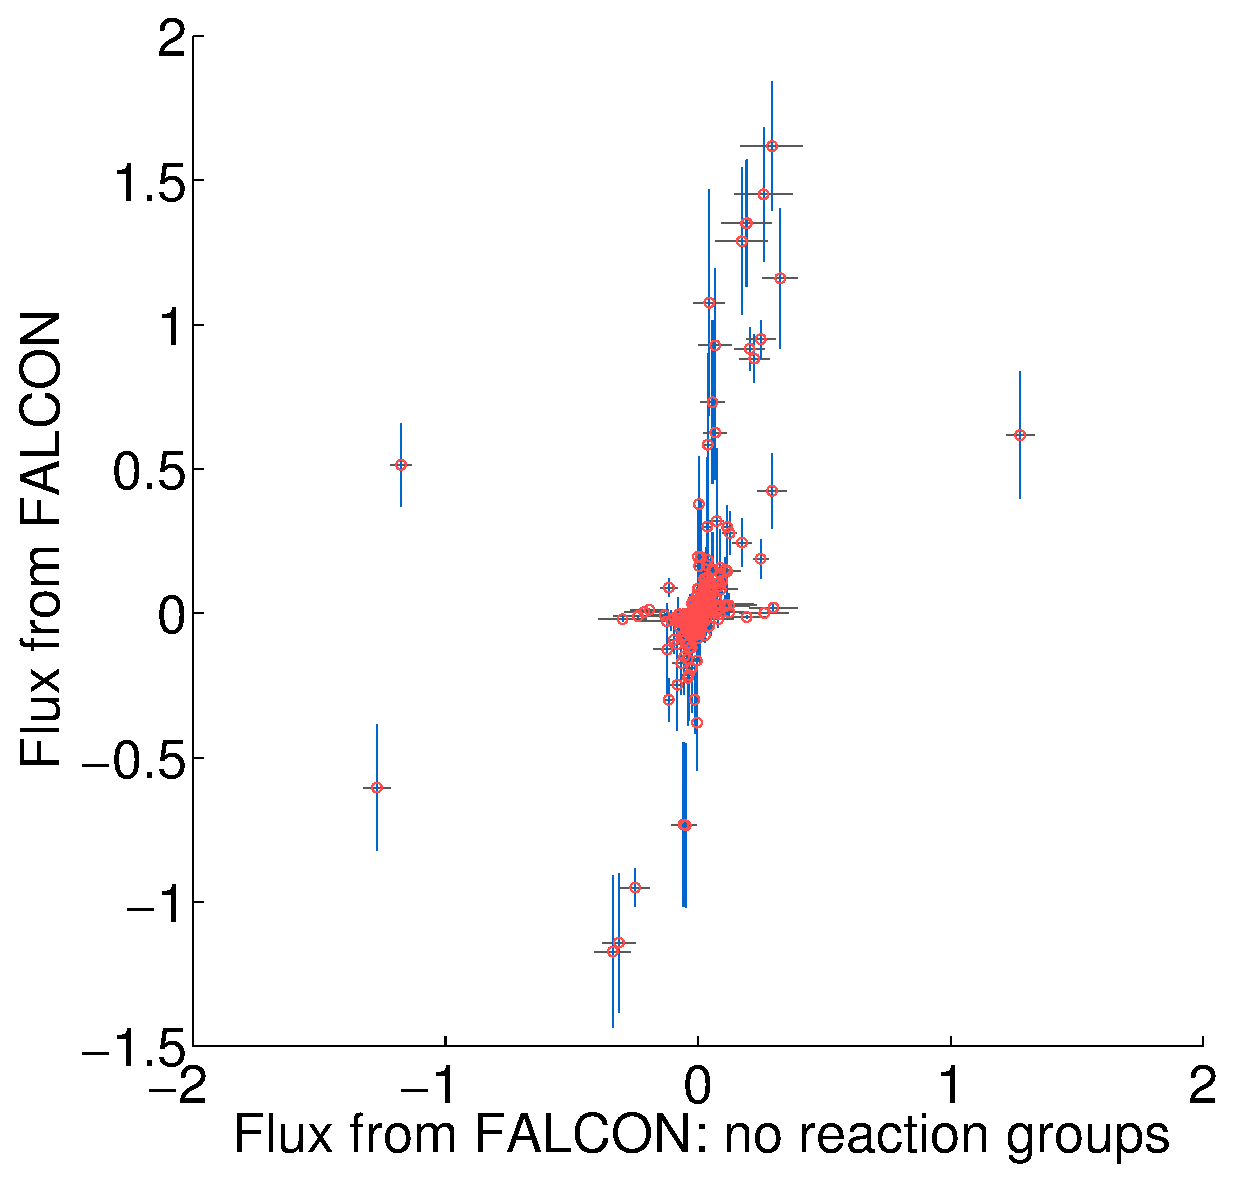
\includegraphics[height=0.7\textheight]
  {falconGrp_yeastMC}
\caption{
Comparison of setting FALCON to use no reaction group information (x-axis)
versus with group information (y-axis; default FALCON setting).}
\label{fig:FalconGrp}
\end{figure}
}

\note{
To emphasize a couple of the points in the previous slide, we can see
that using reaction groups, as opposed to not using them (on the
x-axis), doesn't give us a very good relationship. Additionally, we
can see the error bars in both cases that are due to alternative
optima. The error bars with reaction groups do tend to be larger, likely
due to there being fewer constraints overall, since there's one constraint
per enzyme complex instead of one constraint per reaction.
\par}

%%%%%%%%%%%%%%%%%%%%%%%%%%%%%%%%%%%%%%%%%%%%%%%%%%%%%%%%%%%%%%%%%%%%%%%%%%%%%%%%%%%%%%%%%

\subsection{Performance}

%%%%%%%%%%%%%%%%%%%%%%%%%%%%%%%%%%%%%%%%%%%%%%%%%%%%%%%%%%%%%%%%%%%%%%%%%%%%%%%%%%%%%%%%%%

\frame{\frametitle{Performance} 

\begin{figure}
\newcommand{\hlY}{\cellcolor{Yellow}}
\centering
\resizebox{\textwidth}{!}{%
\begin{tabular}{l*{7}{r}>{\columncolor{Green}}r}
\textbf{(a)} \hspace{1.2cm} & Max. $\mu$ & Model & 
  Standard FBA & Fitted FBA & GIMME & iMAT & Lee et al.      & FALCON\\
 & 75 \%& Yeast~5 MC & 0.66 & 0.66 & NaN  & 0.57 & \hlY 0.64 & 1 \\
 & 75 \%& Yeast~7 MC & 0.66 & 0.66 & 0.68 & 0.66 & \hlY 0.66 & 0.98\\
 & 75 \%& Yeast~5 HC & 0.73 & 0.78 & 0.75 & 0.66 & 0.98      & 0.99\\
Pearson's r  
 & 75 \%& Yeast~7 HC & 0.70 & 0.70 & 0.80 & 0.66 & 0.98      & 0.99\\
 & 85 \%& Yeast~7 MC & 0.62 & 0.62 & 0.65 & 0.62 & \hlY 0.62 & 0.97\\
 & 85 \%& Yeast~5 HC & 0.88 & 0.89 & 0.9  & 0.81 & 0.99      & 0.99\\
 & 85 \%& Yeast~7 HC & 0.67 & 0.67 & 0.87 & 0.62 & 0.98      & 0.98\\
\end{tabular}}
\caption{Performance of FALCON and other CBM methods for predicting
yeast exometabolic fluxes in two growth conditions (75~\% and 85~\%
Max.~$\mu$)}
\label{tab:FalcPerf}
\end{figure}

}

\note{
To evaluate performance, we used a benchmark that
included 7 measured fluxes from yeast in two different conditions
corresponding to 75 and 85 percent of maximum growth rate. We
additionally used two variants (minimally and highly constrained) of
two different versions of a yeast model, to see if any of these
factors largely effected the methods in the panel. While all of
the methods are constraint based methods, the Lee method is the only
similar method to ours (its the one that uses direct evaluation of
gene rules to estimate complex abundance) and can be thought of as the
predecessor. The Lee method performs quite well when the model is
highly constrained, which are the default constraints on directionality
that ship with the yeast model. When these constraints are largely
removed, it loses much of its performance (as shown in yellow),
whereas our method (shown in green) retains good correlation.
\par}


%%%%%%%%%%%%%%%%%%%%%%%%%%%%%%%%%%%%%%%%%%%%%%%%%%%%%%%%%%%%%%%%%%%%%%%%%%%%%%%%%%%%%%%%%%

\frame{\frametitle{Speed} 

\begin{figure}
\centering
\resizebox{\textwidth}{!}{%
\begin{tabular}{l*{6}{r}>{\columncolor{Yellow}}r>{\columncolor{Green}}r}
\textbf{(b)} \hspace{1.2cm} & Max. $\mu$ & Model & 
  Standard FBA & Fitted FBA & GIMME & iMAT & Lee et al. & FALCON\\
 & 75 \%& Yeast~5 MC & 0.9  & 470   & 0.81  & 50     & 110 & 1.8 \\
 & 75 \%& Yeast~7 MC & 1.9  & 3,100 & 2.1   & 12,000 & 600 & 5.6 \\
 & 75 \%& Yeast~5 HC & 0.12 & 110   & 0.18  & 1.4    & 15  & 0.27\\
Time (s) 
 & 75 \%& Yeast~7 HC & 0.72 & 940   & 1.7   & 240    & 670 & 5.5 \\
 & 85 \%& Yeast~7 MC & 2.3  & 3,100 & 3.8   & 14,000 & 610 & 4.6 \\
 & 85 \%& Yeast~5 HC & 0.12 & 110   & 0.18  & 2.5    & 15  & 0.22\\
 & 85 \%& Yeast~7 HC & 0.70 & 110   & 2.5   & 100    & 530 & 5.9\\
\end{tabular}}
\caption{Performance of FALCON and other CBM methods for predicting
yeast exometabolic fluxes in two growth conditions (75~\% and 85~\%
Max.~$\mu$)}
\label{tab:FalcSpeed}
\end{figure}
}


\note{
We also wanted to improve the efficiency of the method, primarily to
get at large models like the human model. In this panel, we only look
at performance on yeast for the same datasets and models as in the
previous slide, but note an increase in performance over Lee.  The Lee and
FALCON methods are really the only good contenders in terms for
correlation, and we see that FALCON has about two orders of magnitude
increase in speed over Lee. The same is true for human models, where
it takes a couple of minutes to estimate a flux with FALCON and over an
hour with the Lee method. All of these benchmarks were done on a single
processor, with the exception of iMAT, which could take quite a while
even on 32 processors.
\par}

%%%%%%%%%%%%%%%%%%%%%%%%%%%%%%%%%%%%%%%%%%%%%%%%%%%%%%%%%%%%%%%%%%%%%%%%%%%%%%%%%%%%%%%%%%

\frame{\frametitle{Permuted expression validates fitting method} 

\begin{figure}
\centering
  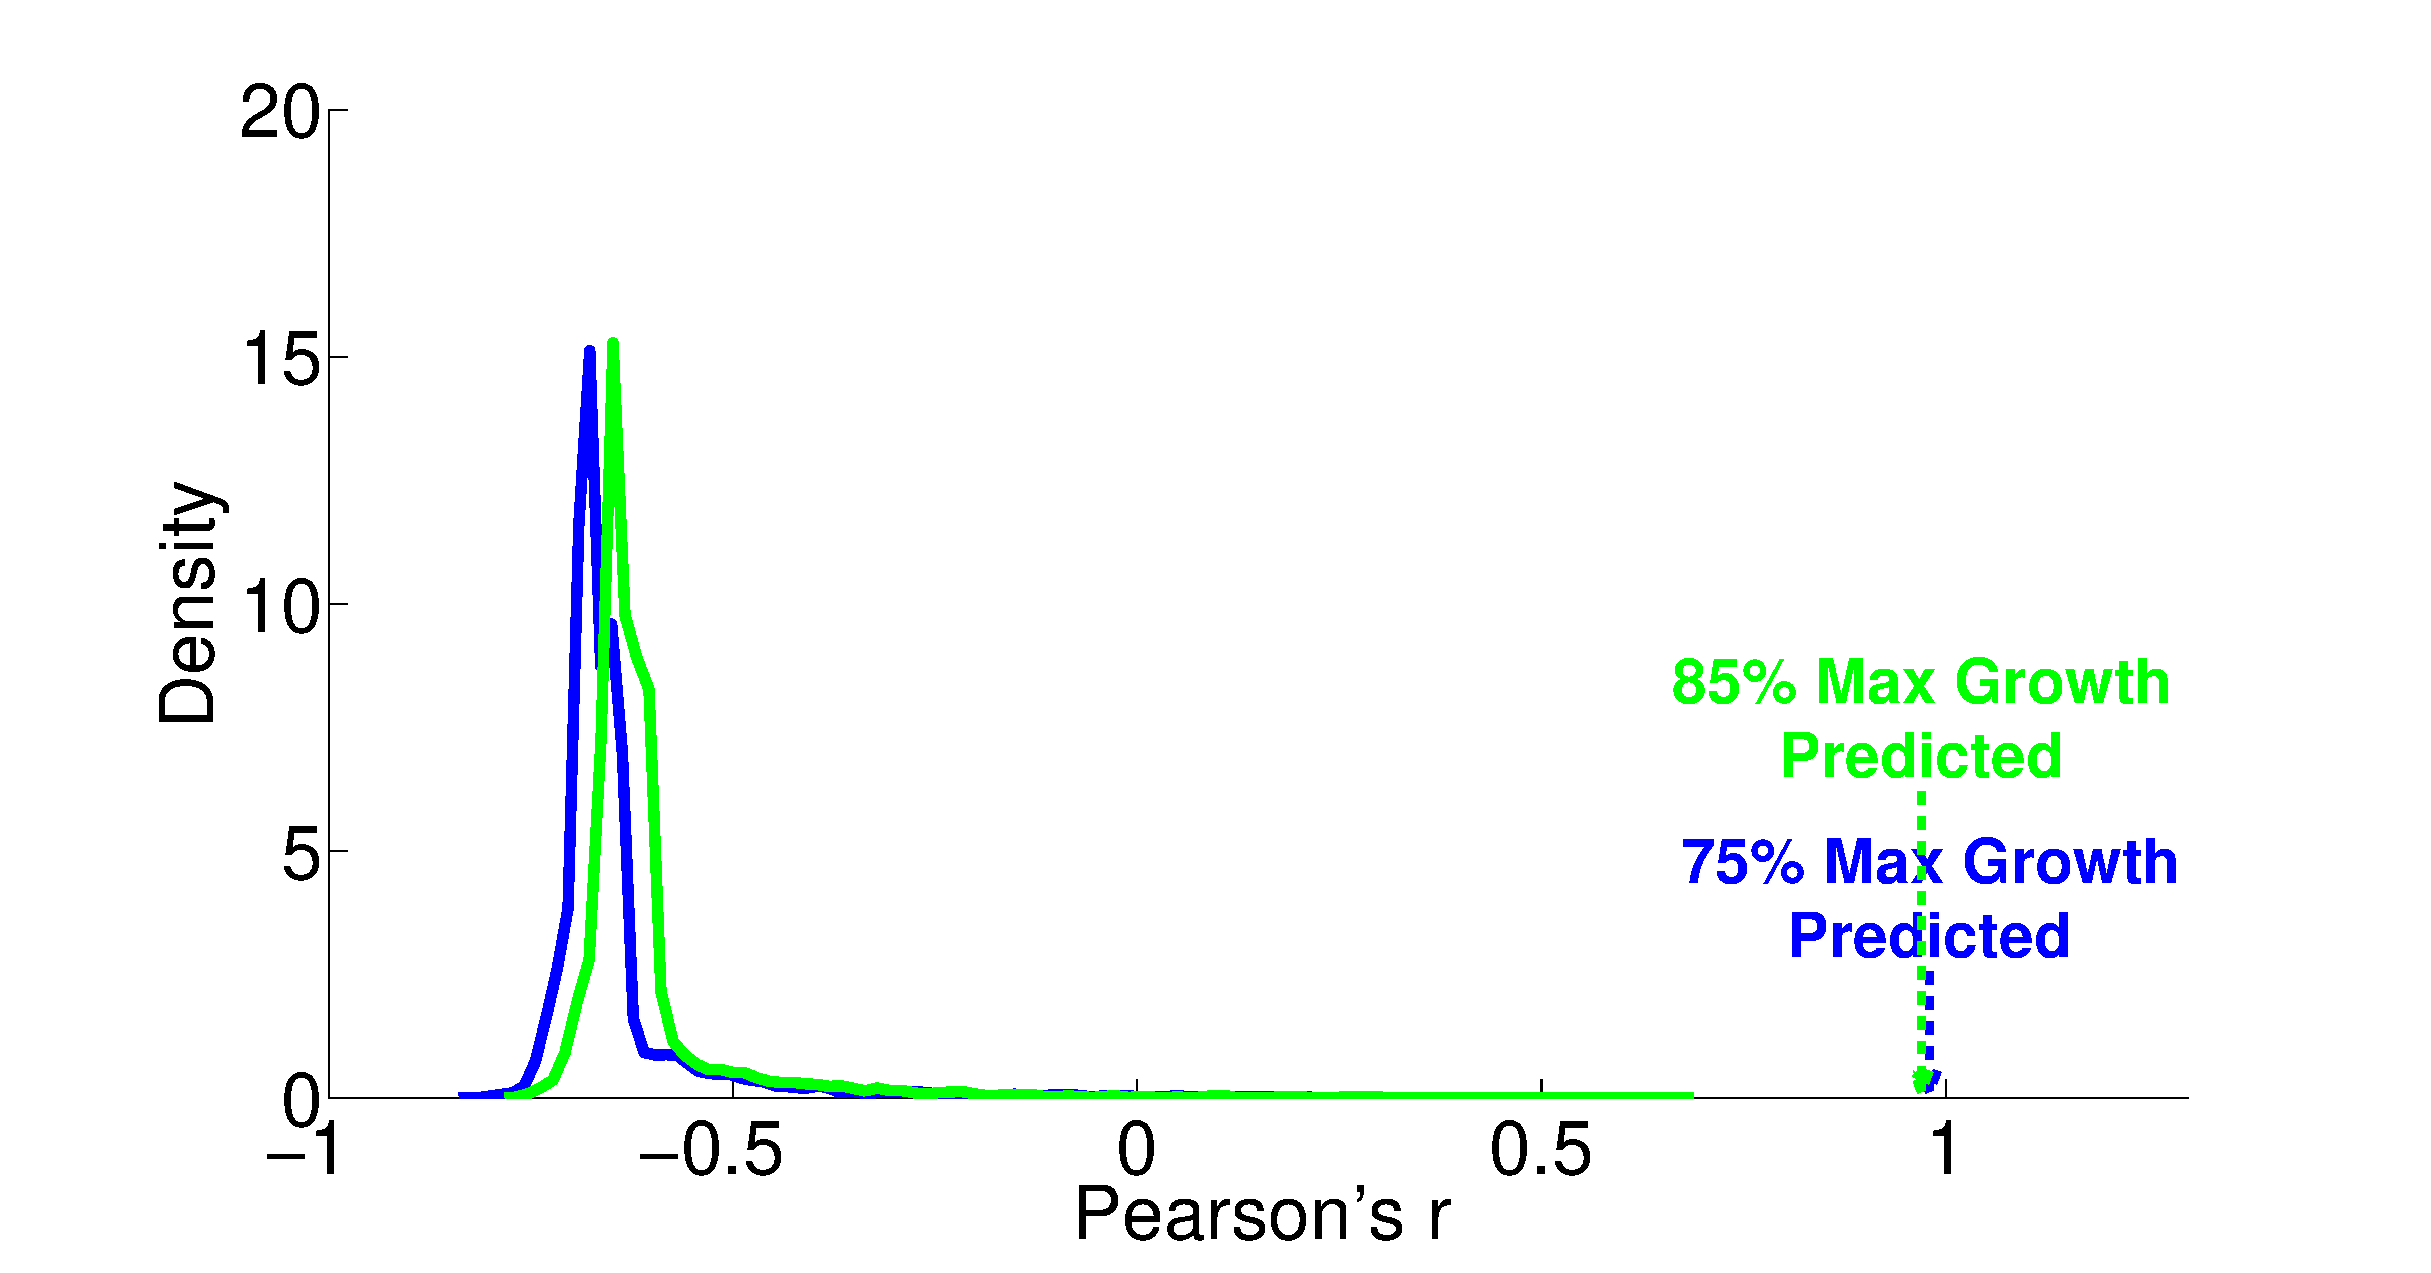
\includegraphics[width=\textwidth]{pExp_dirr}
\caption{PDFs of correlation between experimental fluxes and fluxes
estimated from FALCON when all gene expression data points are
permuted.}
\label{fig:YpermCorr}
\end{figure}
}

\note{ 
We want to be certain that the algorithm actually depends on the input
data in a meaningful way, and that we aren't just getting lucky.  To
demonstrate this, we want to show that garbage in gives
us garbage out.
\par

In order to do this, we randomly permute the input data thousands of
times and feed the it into FALCON and see if the correlation with the
experimental flux data is still good. This gives us a distribution of
correlations, where each correlation corresponds to a single permutation. 
Actually two distributions are plotted here for
different experimental conditions (one green and one blue).
\par

On the far right, we can see the correlations for the two conditions
with unpermuted data, which were the same correlations from the table
we just saw.
\par

Thankfully, we can see that the permuted data does not perform well,
as the distribution shows moderate anti-correlation with the the
empirically measured fluxes.
\par
}


%%%%%%%%%%%%%%%%%%%%%%%%%%%%%%%%%%%%%%%%%%%%%%%%%%%%%%%%%%%%%%%%%%%%%%%%%%%%%%%%%%%%%%%%%%

\frame{\frametitle{An example of noise in the input data} 
\begin{figure}
\centering
  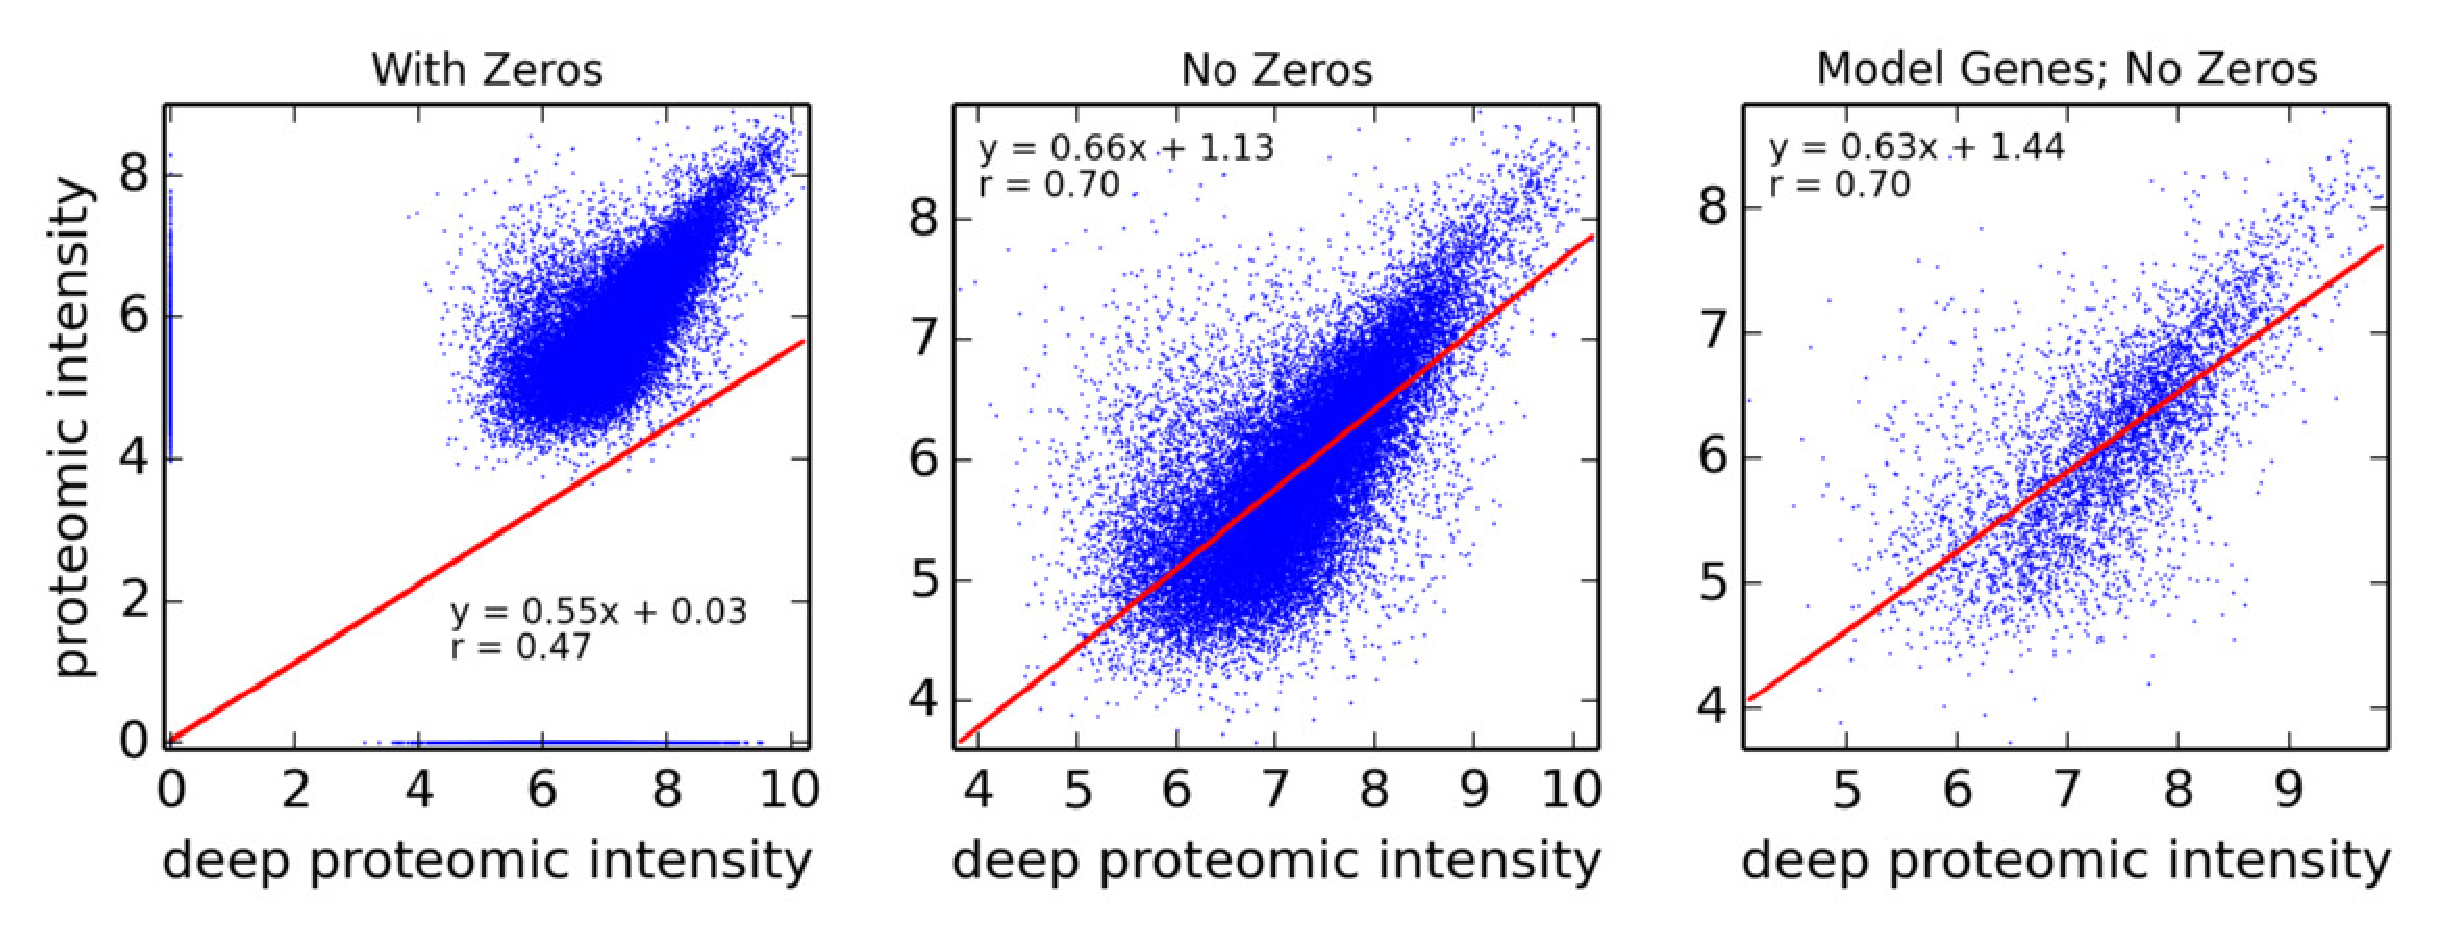
\includegraphics[width=\textwidth]{proteomicComparison}
\caption{Various scatters for two human proteomic datasets for the
same condition.}
\label{fig:protCmp}
\end{figure}
}

\note{ In almost every type of biological data studied today, there is
a certain degree of error. But in high throughput data, even very
noisy data is valuable because there is so much of it. Here is an
example comparison of two proteomic data sets taken from the same cell
types but using different instruments to measure protein
intensity. I've removed all pairs with a zero value in the middle figure,
and additionally all non-metabolic genes in the last figure. 
The important thing to note in these three schemes
is that, while there is a correlation, there is also a fair amount of
noise. We need to make sure our algorithm is capable of handling a
reasonable amount of noise.}


%%%%%%%%%%%%%%%%%%%%%%%%%%%%%%%%%%%%%%%%%%%%%%%%%%%%%%%%%%%%%%%%%%%%%%%%%%%%%%%%%%%%%%%%%%

\frame{\frametitle{Sensitivity to expression noise} 
\begin{figure}
\centering
  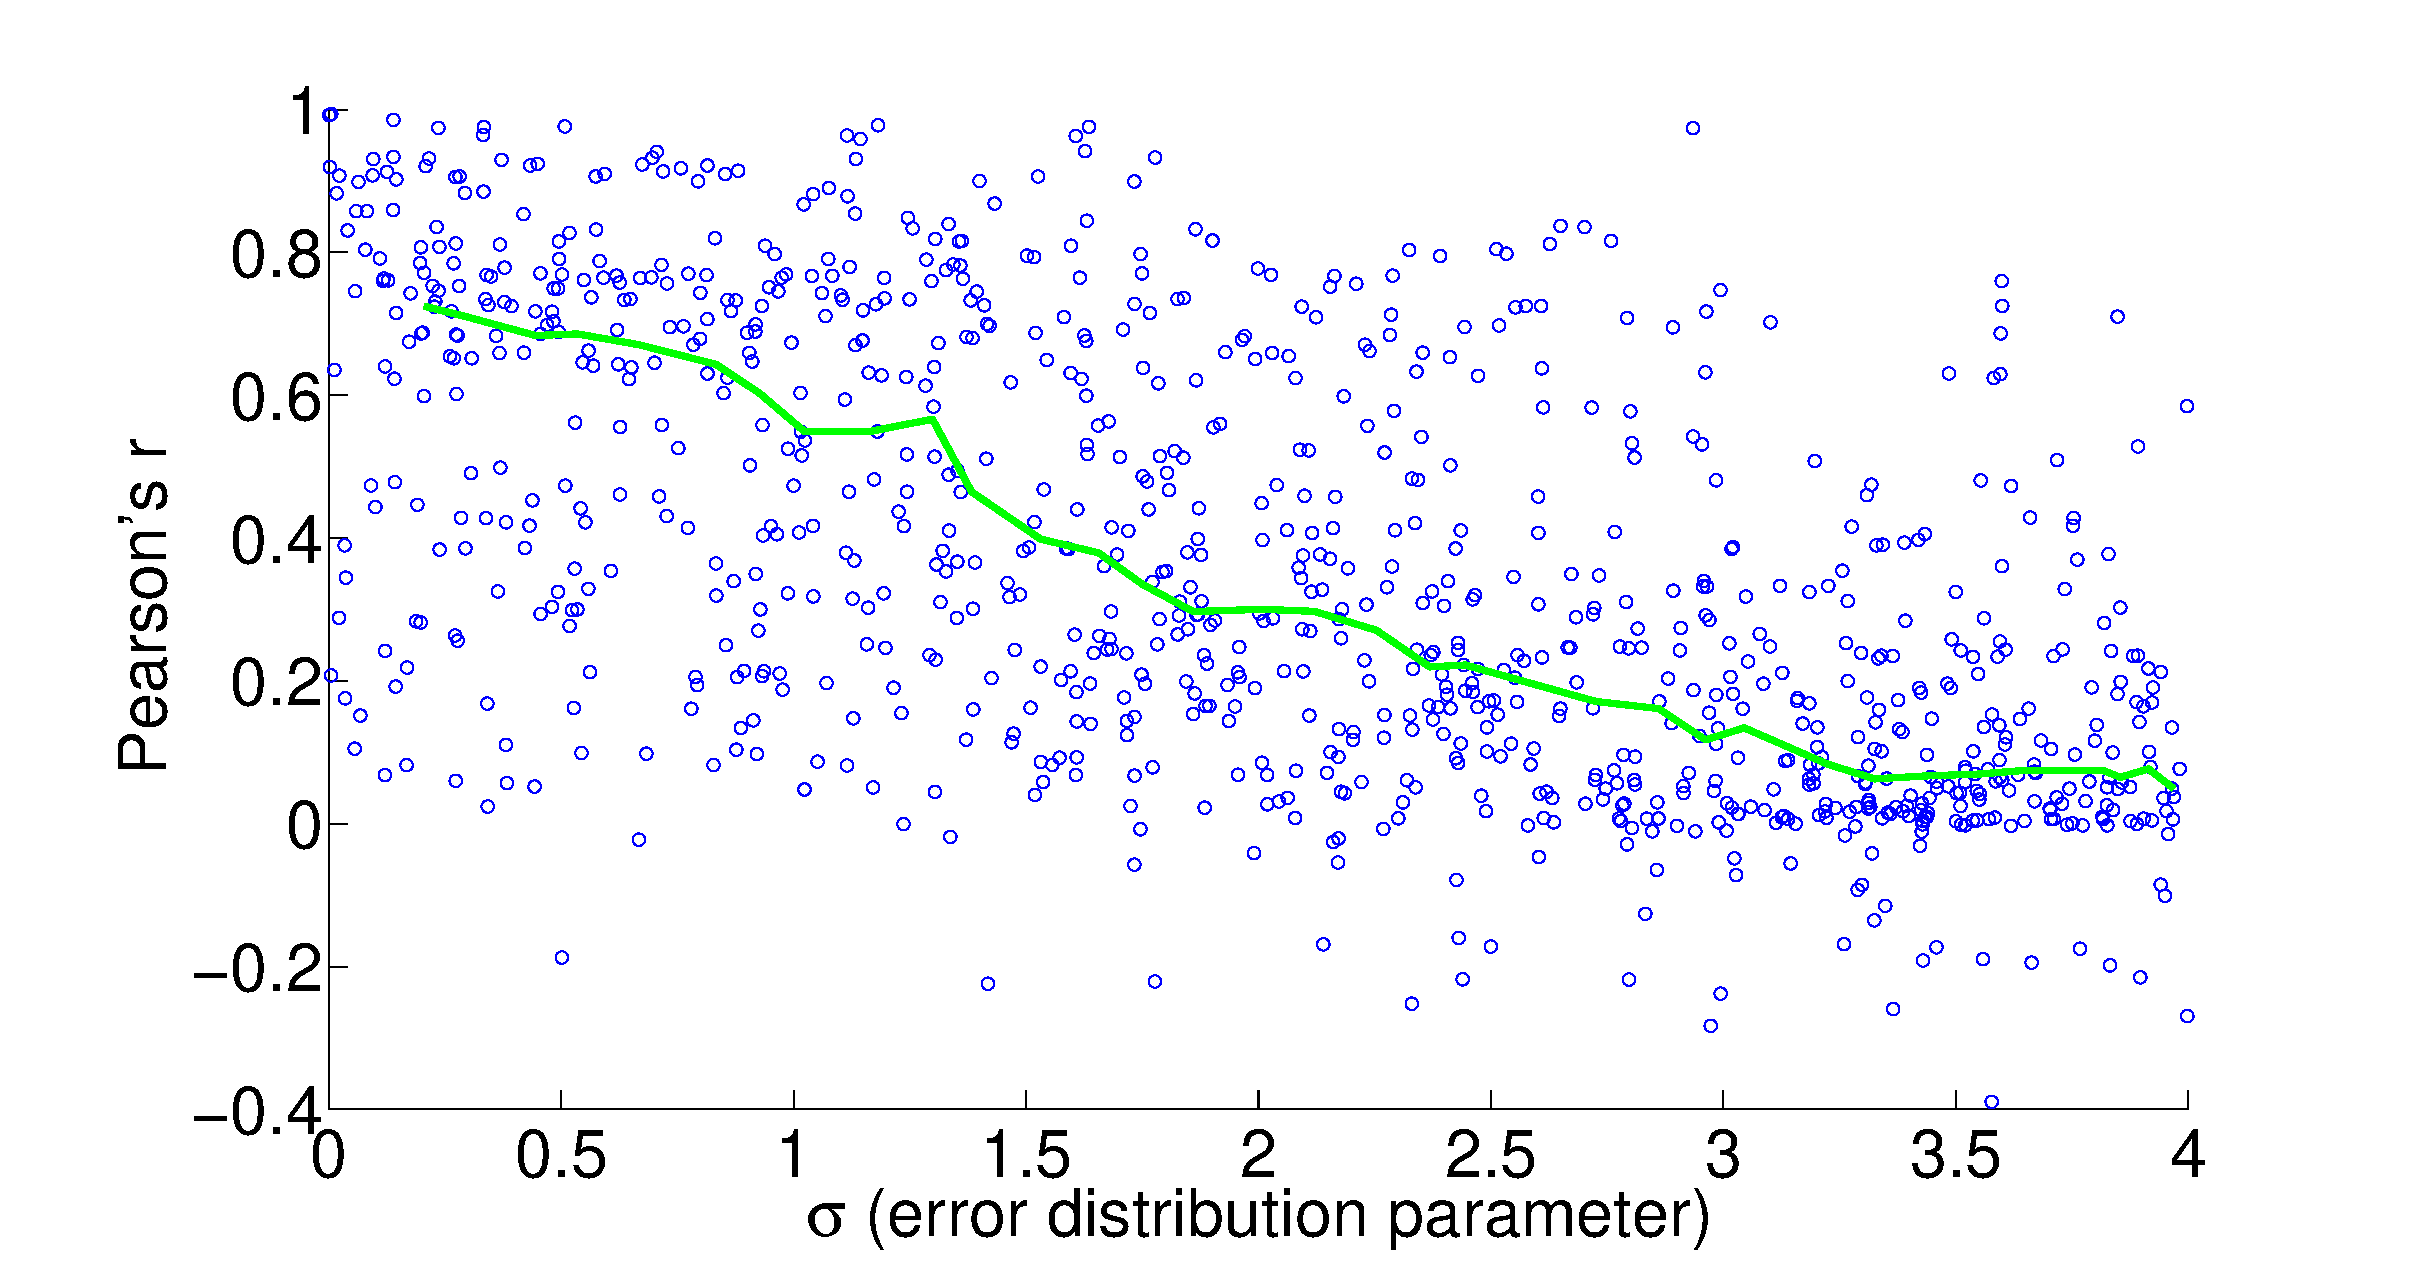
\includegraphics[width=\textwidth]{noise_y7MCflux}
\caption{Correlation of flux vectors estimated from perturbed versus
unperturbed complex abundance for the Yeast~7 model.}
\label{fig:ExpSens}
\end{figure}
}

\note{
In order to evaluate the sensitivity of FALCON to noise, we can
multiply the enzyme complex abundance values by randomly sampled noise
from a multivariate log-normal distribution with parameter
$\sigma$. The larger the $\sigma$, the more noise there will be. In
this figure, you see the $\sigma$ on the x-axis, and the corresponding
correlation between flux vectors estimated based on the perturbed and
unperturbed enzyme complex abundance. The green line is the interval
median correlation.

In the previous slide, we saw a Pearson's $r$ of 0.7 for the input
data. This corresponds roughly to a $\sigma$ of 1.25, so that on
average, we might expect an $r$ of about 0.6 in the output data, that is,
in the flux. But, it is obvious that the worst case is much worse.
The good news is that we can take model annotations of known
constraints and reduce the sensitivity even further.
\par}


%%%%%%%%%%%%%%%%%%%%%%%%%%%%%%%%%%%%%%%%%%%%%%%%%%%%%%%%%%%%%%%%%%%%%%%%%%%%%%%%%%%%%%%%%%

\frame{\frametitle{Sensitivity to expression noise: Highly Constrained} 
\begin{figure}
\centering
  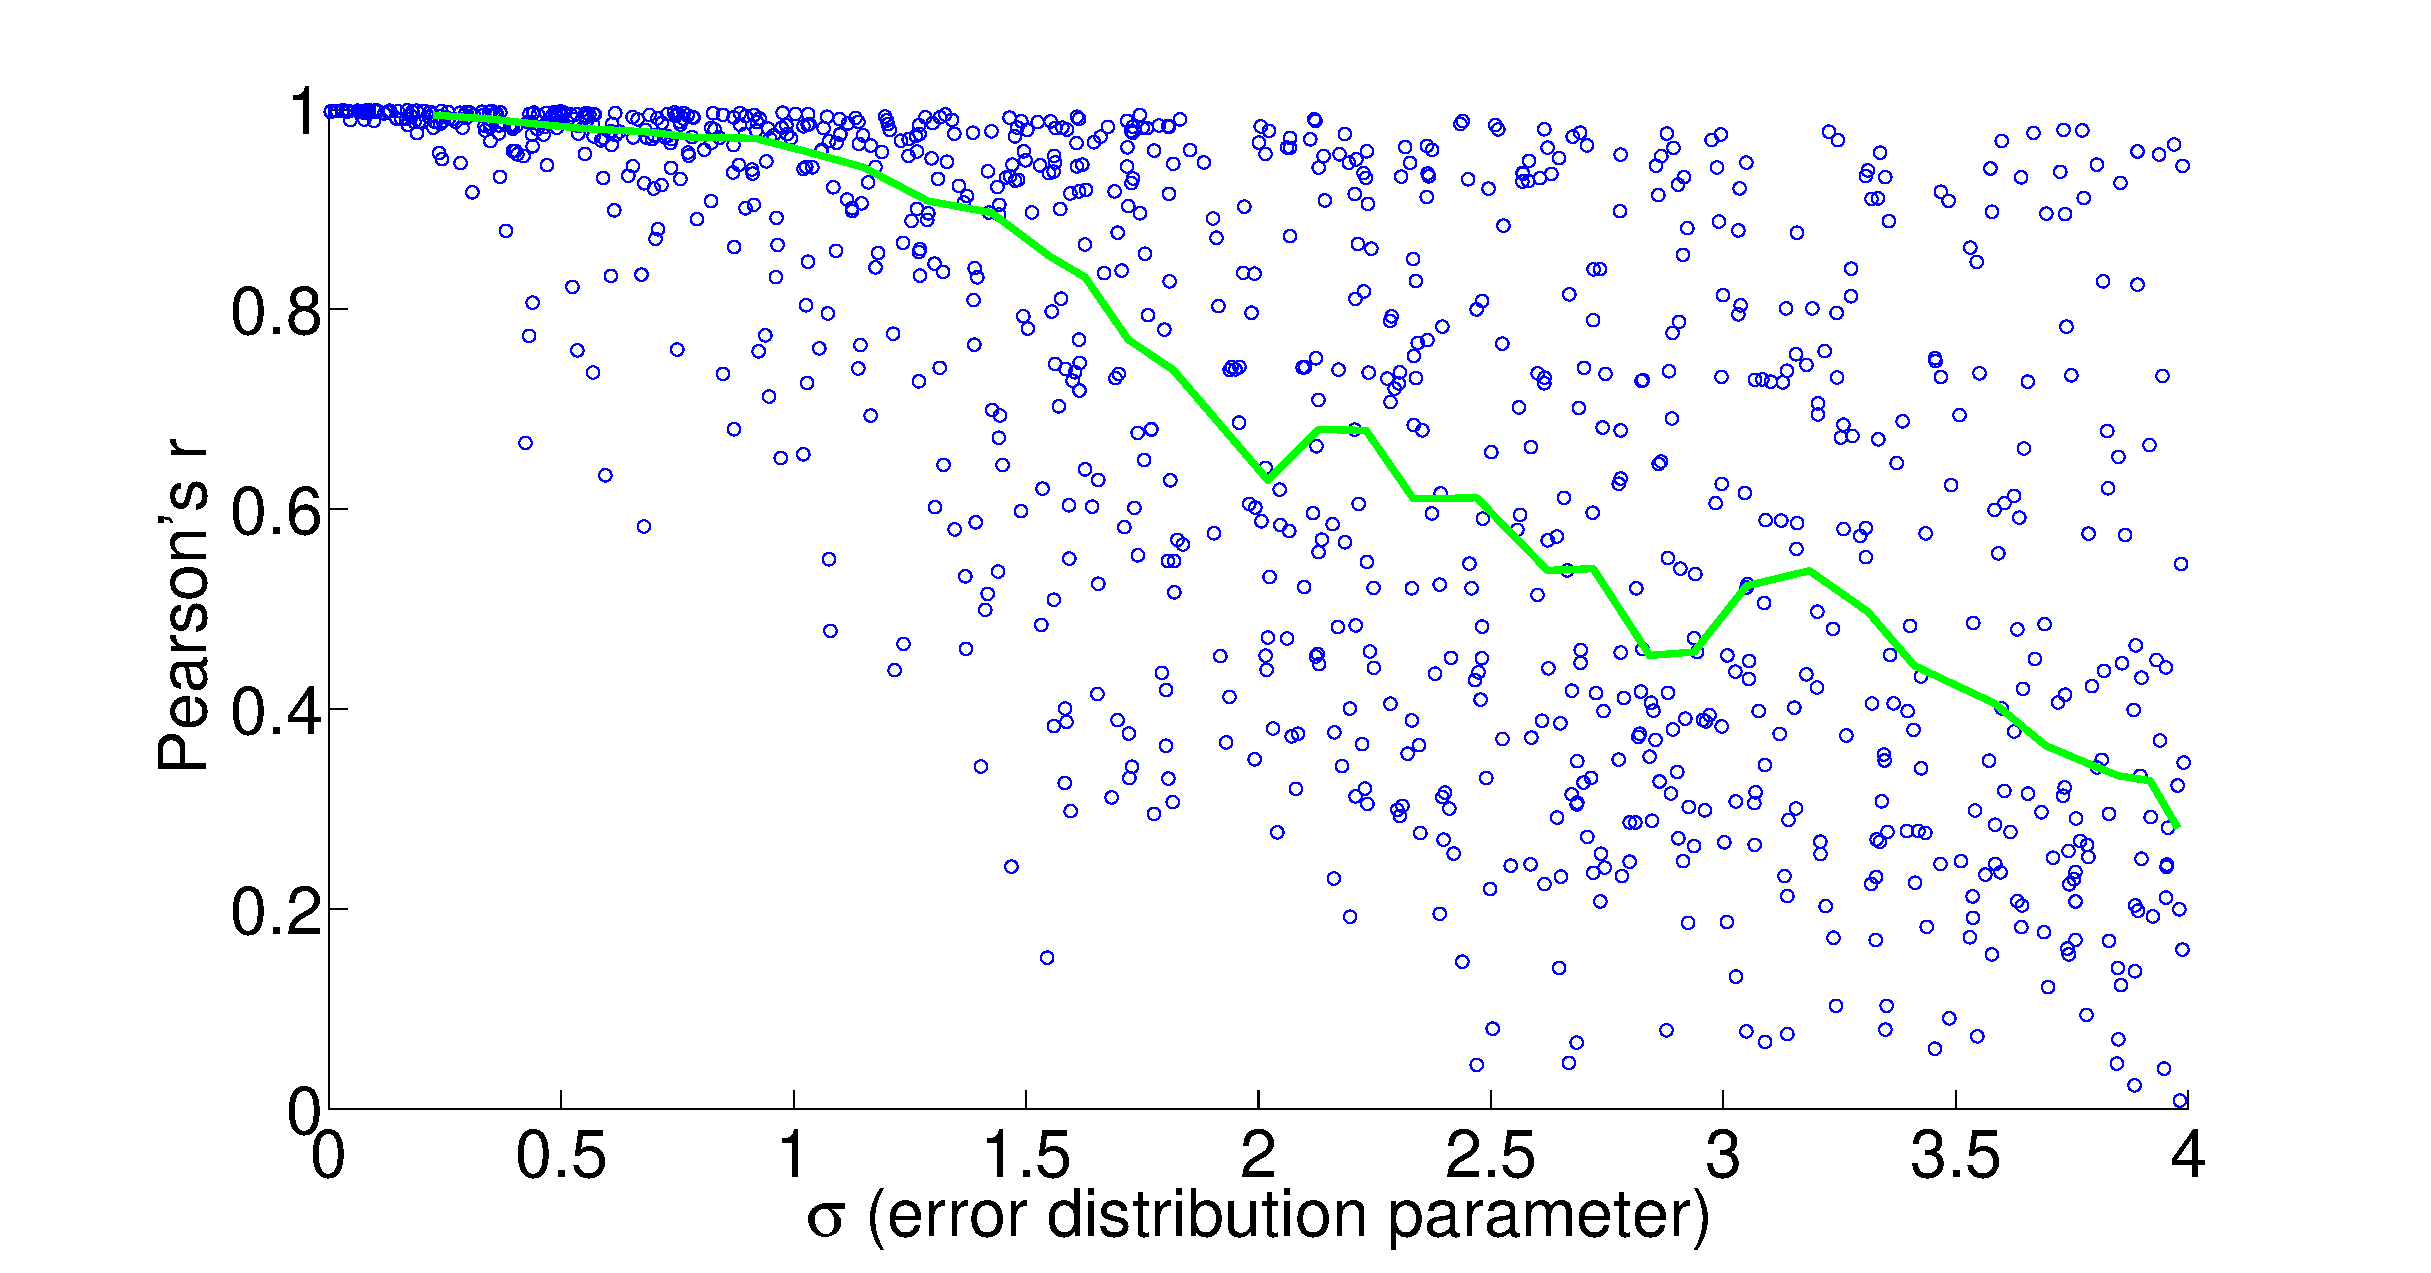
\includegraphics[width=\textwidth]{noise_y7HCflux}
\caption{Correlation of flux vectors estimated from perturbed versus
unperturbed complex abundance for the Yeast~7 model.}
\label{fig:ExpSensH}
\end{figure}
}

\note{In this example for yeast, we restored all of the known reaction
directions from the model, and we now see that for a $\sigma$ of 1.25,
we can expect an $r$ of nearly 0.95, and the number of poor
correlations in output at this $\sigma$ level is much less than in the
previous slide. We wanted to test both constraint sets because many
models are not as well understood as yeast, hence the reactions may be 
annotated as being reversible. Additionally, reaction
direction may change depending on environmental conditions, so it is
good to know how far we can get with a deconstrained model.
}

%%%%%%%%%%%%%%%%%%%%%%%%%%%%%%%%%%%%%%%%%%%%%%%%%%%%%%%%%%%%%%%%%%%%%%%%%%%%%%%%%%%%%%%%%%

\frame{\frametitle{Thank you!} 


\begin{columns}[t]
%
\begin{column}{0.5\textwidth}
\ul{\textit{Co-authors}}
\begin{itemize}
\item Zhenglong Gu
\item Jason W. Locasale
\item Christopher R. Myers
\item Narayanan Sadagopan
\item Kieran Smallbone
\item Yiping Wang
\item Hongwei Xi
\item Lin Xu
\end{itemize}
\end{column}

\begin{column}{0.5\textwidth}
\ul{\textit{Other thanks}}
\begin{itemize}
\item David Christini 
\item Paul Billing-Ross
\item Michael Stillman
\item Neil Swainston
\item Kaixiong Ye
\item Tri-I CBM
\item Cornell's CAC
\end{itemize}

\vspace{0.2in}
\TriILogo{0.6in}

\end{column}

%
\end{columns}
}

\note{

Finally, thank you all for listening and having mere here today.  I'd
like to also credit my co-authors who helped make the work as strong as
it is, as well as several members of my committee and my lab,
especially Lin Xu who really introduced me to a lot of exciting ideas
in biology.

}

%%%%%%%%%%%%%%%%%%%%%%%%%%%%%%%%%%%%%%%%%%%%%%%%%%%%%%%%%%%%%%%%%%%%%%%%%%%%%%%%%%%%%%%%%%

%%%%%%%%%%%%%%%%%%%%%%%%%%%%%%%%
                               %
\section[]{Additional Slides}  %
                               %
%%%%%%%%%%%%%%%%%%%%%%%%%%%%%%%%

%%%%%%%%%%%%%%%%%%%%%%%%%%%%%%%%%%%%%%%%%%%%%%%%%%%%%%%%%%%%%%%%%%%%%%%%%%%%%%%%%%%%%%%%%%

\frame{\frametitle{}} %blank slide

%%%%%%%%%%%%%%%%%%%%%%%%%%%%%%%%%%%%%%%%%%%%%%%%%%%%%%%%%%%%%%%%%%%%%%%%%%%%%%%%%%%%%%%%%%

\frame{\frametitle{Distribution of \textit{in silico} samples of mutant allele pairs
where the more severe mutant exhibits prevalent negative epistasis.} 

\begin{figure}
\centering
  \includegraphics[height=0.65\textheight, viewport=50 200 376 409, clip=true]
  {sgeFigure_2}
\label{fig:ExpFBAconfirm:B}
\end{figure}
}

%%%%%%%%%%%%%%%%%%%%%%%%%%%%%%%%%%%%%%%%%%%%%%%%%%%%%%%%%%%%%%%%%%%%%%%%%%%%%%%%%%%%%%%%%%

\frame{\frametitle{Prevalent negative epistasis in severe mutants is robust across
parameter selection.} 

\begin{figure}
\centering
  \includegraphics[width=\textwidth, viewport=16 7 434 189, clip=true]
  {sgeFigure_2}
\label{fig:ExpFBAconfirm:C}
\end{figure}
}

%%%%%%%%%%%%%%%%%%%%%%%%%%%%%%%%%%%%%%%%%%%%%%%%%%%%%%%%%%%%%%%%%%%%%%%%%%%%%%%%%%%%%%%%%%

\frame{\frametitle{Increased efficiency of purging deleterious mutations in
eukaryotic organisms} 
\framesubtitle{Population genetic model for allele
frequency changes from generation to generation}

\begin{figure}
\centering
  \includegraphics[width=\textwidth, viewport=11 475 519 663, clip=true]
  {sgeFigure_4}
\label{fig:sgePopGen:A}
\end{figure}
}

%%%%%%%%%%%%%%%%%%%%%%%%%%%%%%%%%%%%%%%%%%%%%%%%%%%%%%%%%%%%%%%%%%%%%%%%%%%%%%%%%%%%%%%%%%


\newsavebox{\popgenRow}
\newsavebox{\popgenXlabel}
\newsavebox{\popgenYlabel}
\newsavebox{\popgenYlabelTop}

\newlength{\popgenRowWid}
\setlength{\popgenRowWid}{0.95\textwidth}


\frame{\frametitle{Increased efficiency of mutation purging in
eukaryotic organisms: ratio of severe to weak gene-A alleles}
\framesubtitle{%
\only<1>{The 50th, 100th, and 150th generations}%
\only<2>{The 200th, 250th, and 300th generations}%
}



\savebox{\popgenRow}{%
\includegraphics<1>[width=\popgenRowWid, viewport=51 276 479 407, clip=true]
{sgeFigure_4}%
\includegraphics<2>[width=\popgenRowWid, viewport=51 141 479 269, clip=true]
{sgeFigure_4}%
}

\savebox{\popgenXlabel}{%
\includegraphics[width=\popgenRowWid, viewport=68 11 491 114, clip=true]
{sgeFigure_4}%
}

\savebox{\popgenYlabel}{%
\includegraphics[width=0.035\textwidth, viewport=29 136 43 276, clip=true]
{sgeFigure_4}%
}

\savebox{\popgenYlabelTop}{\scriptsize%
\hspace{-0.0cm}%
\only<1>{\hspace{1.1cm}50th Generation \hspace{1em}\hspace{1.1cm}%
  100th Generation \hspace{1cm} 150th Generation}%
\only<2>{\hspace{1.1cm}200th Generation            \hspace{1.1cm}%
  250th Generation \hspace{1.1cm} 300th Generation}%
}

% % % %

\begin{picture}(\textwidth, \textheight)

\put(0.05\textwidth, 0.35\textheight){%
  \makebox(\popgenRowWid, 0.55\textheight)[lt]{\usebox{\popgenRow}}}

\put(0.08\textwidth, 0.3\textheight){%
  \makebox(\popgenRowWid, 0.25\textheight)[lt]{\usebox{\popgenXlabel}}}

\put(0.0\textwidth, 0.37\textheight){%
  \makebox(0.05\textwidth, 0.55\textheight)[lt]{\usebox{\popgenYlabel}}}

\put(0.05\textwidth, 0.88\textheight){%
  \makebox(\popgenRowWid, 0.05\textheight)[lt]{\usebox{\popgenYlabelTop}}}

\end{picture}

} % end of \frame

%%%%%%%%%%%%%%%%%%%%%%%%%%%%%%%%%%%%%%%%%%%%%%%%%%%%%%%%%%%%%%%%%%%%%%%%%%%%%%%%%%%%%%%%%%


\begin{frame}[fragile]
\frametitle{Gene-rule API examples}

\begin{columns}
%
\begin{column}{0.5\textwidth}
\lstinputlisting[basicstyle=\ttfamily\tiny, language=ATS, showstringspaces=false]
{\commonDir falcon_main_fun.dats}
\end{column}
%
\vrule{}
%
\begin{column}{0.5\textwidth}
\lstinputlisting[basicstyle=\ttfamily\tiny, language=ATS, showstringspaces=false]
{\commonDir falcon_example.dats}
\end{column}
%
\end{columns}
\end{frame}

%%%%%%%%%%%%%%%%%%%%%%%%%%%%%%%%%%%%%%%%%%%%%%%%%%%%%%%%%%%%%%%%%%%%%%%%%%%%%%%%%%%%%%%%%%

\begin{frame}[fragile]
\frametitle{Enzyme complex abundance estimating with CNF}

\begin{algorithm}[H]
\scriptsize
\caption{CNF-izing min disjunction}
\label{alg:ReductionToCNF}
\begin{algorithmic}
%\ifthenelse{\boolean{thesisStyle}}{\singlespacing}{}
\INPUT $G = \left\{g_i~\mid~i \in{1, \ldots, m}\right\}$ are genes. 
\INPUT $r$ := A Boolean rule without negation consisting of\\
  $\left\{x_i~\mid~i \in{1, \ldots, n}\right\}$ Boolean sub-expressions.
\INPUT $\E{g}$ := A map returning the expression level of gene g.
\While{$rule \neq o_1 \land \ldots \land o_p$ where each $o_i$ is a disjunction
  of genes} 
  \If {Encounter a disjunction $x_d$ of conjunctions of genes}
  \State \parbox[t]{\dimexpr\linewidth-\algorithmicindent}{
    Create sets from conjunctions, i.e.:\\
    Create $G_1$ and $G_2$ with $g_{1,i} \in G_1$ 
    and $g_{2,i} \in G_2$ where\\ 
    $x_d = (g_{1,1} \land \ldots \land g_{1,r}) \lor 
    (g_{2,1} \land \ldots \land g_{2,s})$. 
    \strut}
    \If {$G_1 \subseteq G_2$}
    \State Replace $x_d$ with $(g_{1,1} \land \ldots \land g_{1,r})$.
    \ElsIf {$G_2 \subseteq G_1$}
    \State Replace $x_d$ with $(g_{2,1} \land \ldots \land g_{2,s})$.
    \EndIf 
  \EndIf
  \State \parbox[t]{\dimexpr\linewidth-\algorithmicindent}{
    Distribute $\lor$ over $\land$, e.g.: $(x_1 \land x_2) \lor (x_3 \land x_4)$ \\ 
    $\rightarrow (x_1 \lor x_3) \land (x_1 \lor x_4) \land 
    (x_2 \lor x_3) \land (x_2 \lor x_4)$
    \strut}
\EndWhile
\OUTPUT $o_{\min}$ where $o_{\min}$ has the form: $\ORw_{g_i \in G} g_i$ (uses $\E{g}$)
\end{algorithmic} 
\end{algorithm}

\end{frame}

%%%%%%%%%%%%%%%%%%%%%%%%%%%%%%%%%%%%%%%%%%%%%%%%%%%%%%%%%%%%%%%%%%%%%%%%%%%%%%%%%%%%%%%%%%

\begin{frame}[fragile]
\frametitle{The FALCON flux-fitting algorithm}

\begin{algorithm}[H]
\tiny
\caption{FALCON}
\label{alg:FALCON}
\begin{algorithmic}
%\ifthenelse{\boolean{thesisStyle}}{\singlespacing}{}
\State $u_{\min} := \min_j\ \{V_{j,\max} : V_{j,\max} > 0\}$
\State $V_{lb}^{\Sigma} := u_{\min} \left|\{v_j : e_j \textnormal{ exists}\}\right|$
\State {Scale data to be of similar size for numeric stability:}
\ForAll {j}
  \State $e_j := \frac{e_j V_{lb}^{\Sigma}}
    {\sum\limits_{j} e_j}$ 
  \State $\sigma_j := \frac{\sigma_j V_{lb}^{\Sigma}}
    {\sum\limits_{j} e_j}$
\EndFor
\While{$rxns_{irrev} > rxns_{irrev,prior}$}
  \State {$rxns_{irrev,prior} := rxns_{irrev}$}
  \State Call LP Solver:
  \State \hspace{4.8mm} \parbox[t]{\dimexpr\linewidth-\algorithmicindent}{
    $\textnormal{minimize}\ \sum\limits_i \frac{d_i}{n \sigma_i}$\\
    s.t.\\
    $\sum_{j \mid e_j \textnormal{ exists }} v_j \geq V_{lb}^{\Sigma}$\\ 
    $\forall i: -d_i \leq \sum\nolimits_{j \in R_i} (v_{j,f} +
    v_{j,b}) - n e_i \leq d_i$\\ 
    $d_i, v_{j,f}, v_{j,b} \geq 0$\\ 
    $n > 0$
    \strut}
  \ForAll {$\left\{j \mid v_{j,f} + v_{j,b} > 0, v_{j,f} \neq v_{j,b} \right\}$}
  \State {Constrain the smaller of $v_{j,f}$ and $v_{j,b}$ to be $0$.}  
  \State {$rxns_{irrev}$++}
  \EndFor
\EndWhile
\end{algorithmic}
\end{algorithm}

\end{frame}

%%%%%%%%%%%%%%%%%%%%%%%%%%%%%%%%%%%%%%%%%%%%%%%%%%%%%%%%%%%%%%%%%%%%%%%%%%%%%%%%%%%%%%%%%%

\frame{\frametitle{Grouping reactions by enzyme complex: HC} 

\begin{figure}
\centering
  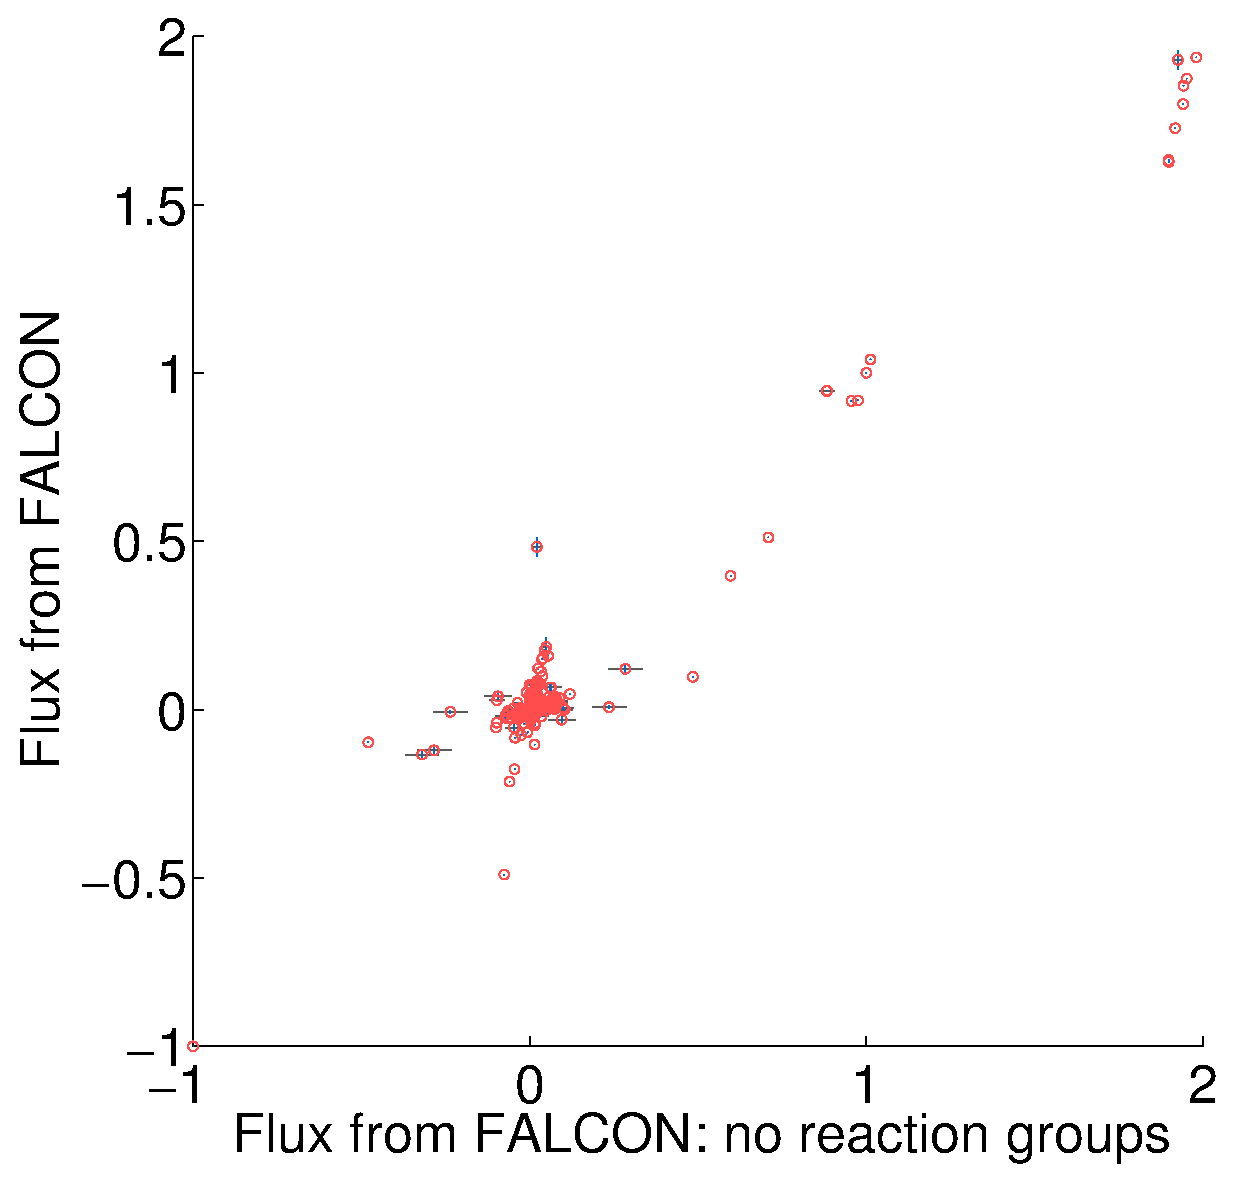
\includegraphics[height=0.65\textheight]
  {falconGrp_yeastHC}
\caption{
Comparison of setting FALCON to use no reaction group information (x-axis)
versus with group information (y-axis; default FALCON setting).}
\label{fig:FalconGrpH}
\end{figure}
}

%%%%%%%%%%%%%%%%%%%%%%%%%%%%%%%%%%%%%%%%%%%%%%%%%%%%%%%%%%%%%%%%%%%%%%%%%%%%%%%%%%%%%%%%%%

\frame{\frametitle{Permuted expression validates fitting method: HC} 

\begin{figure}
\centering
  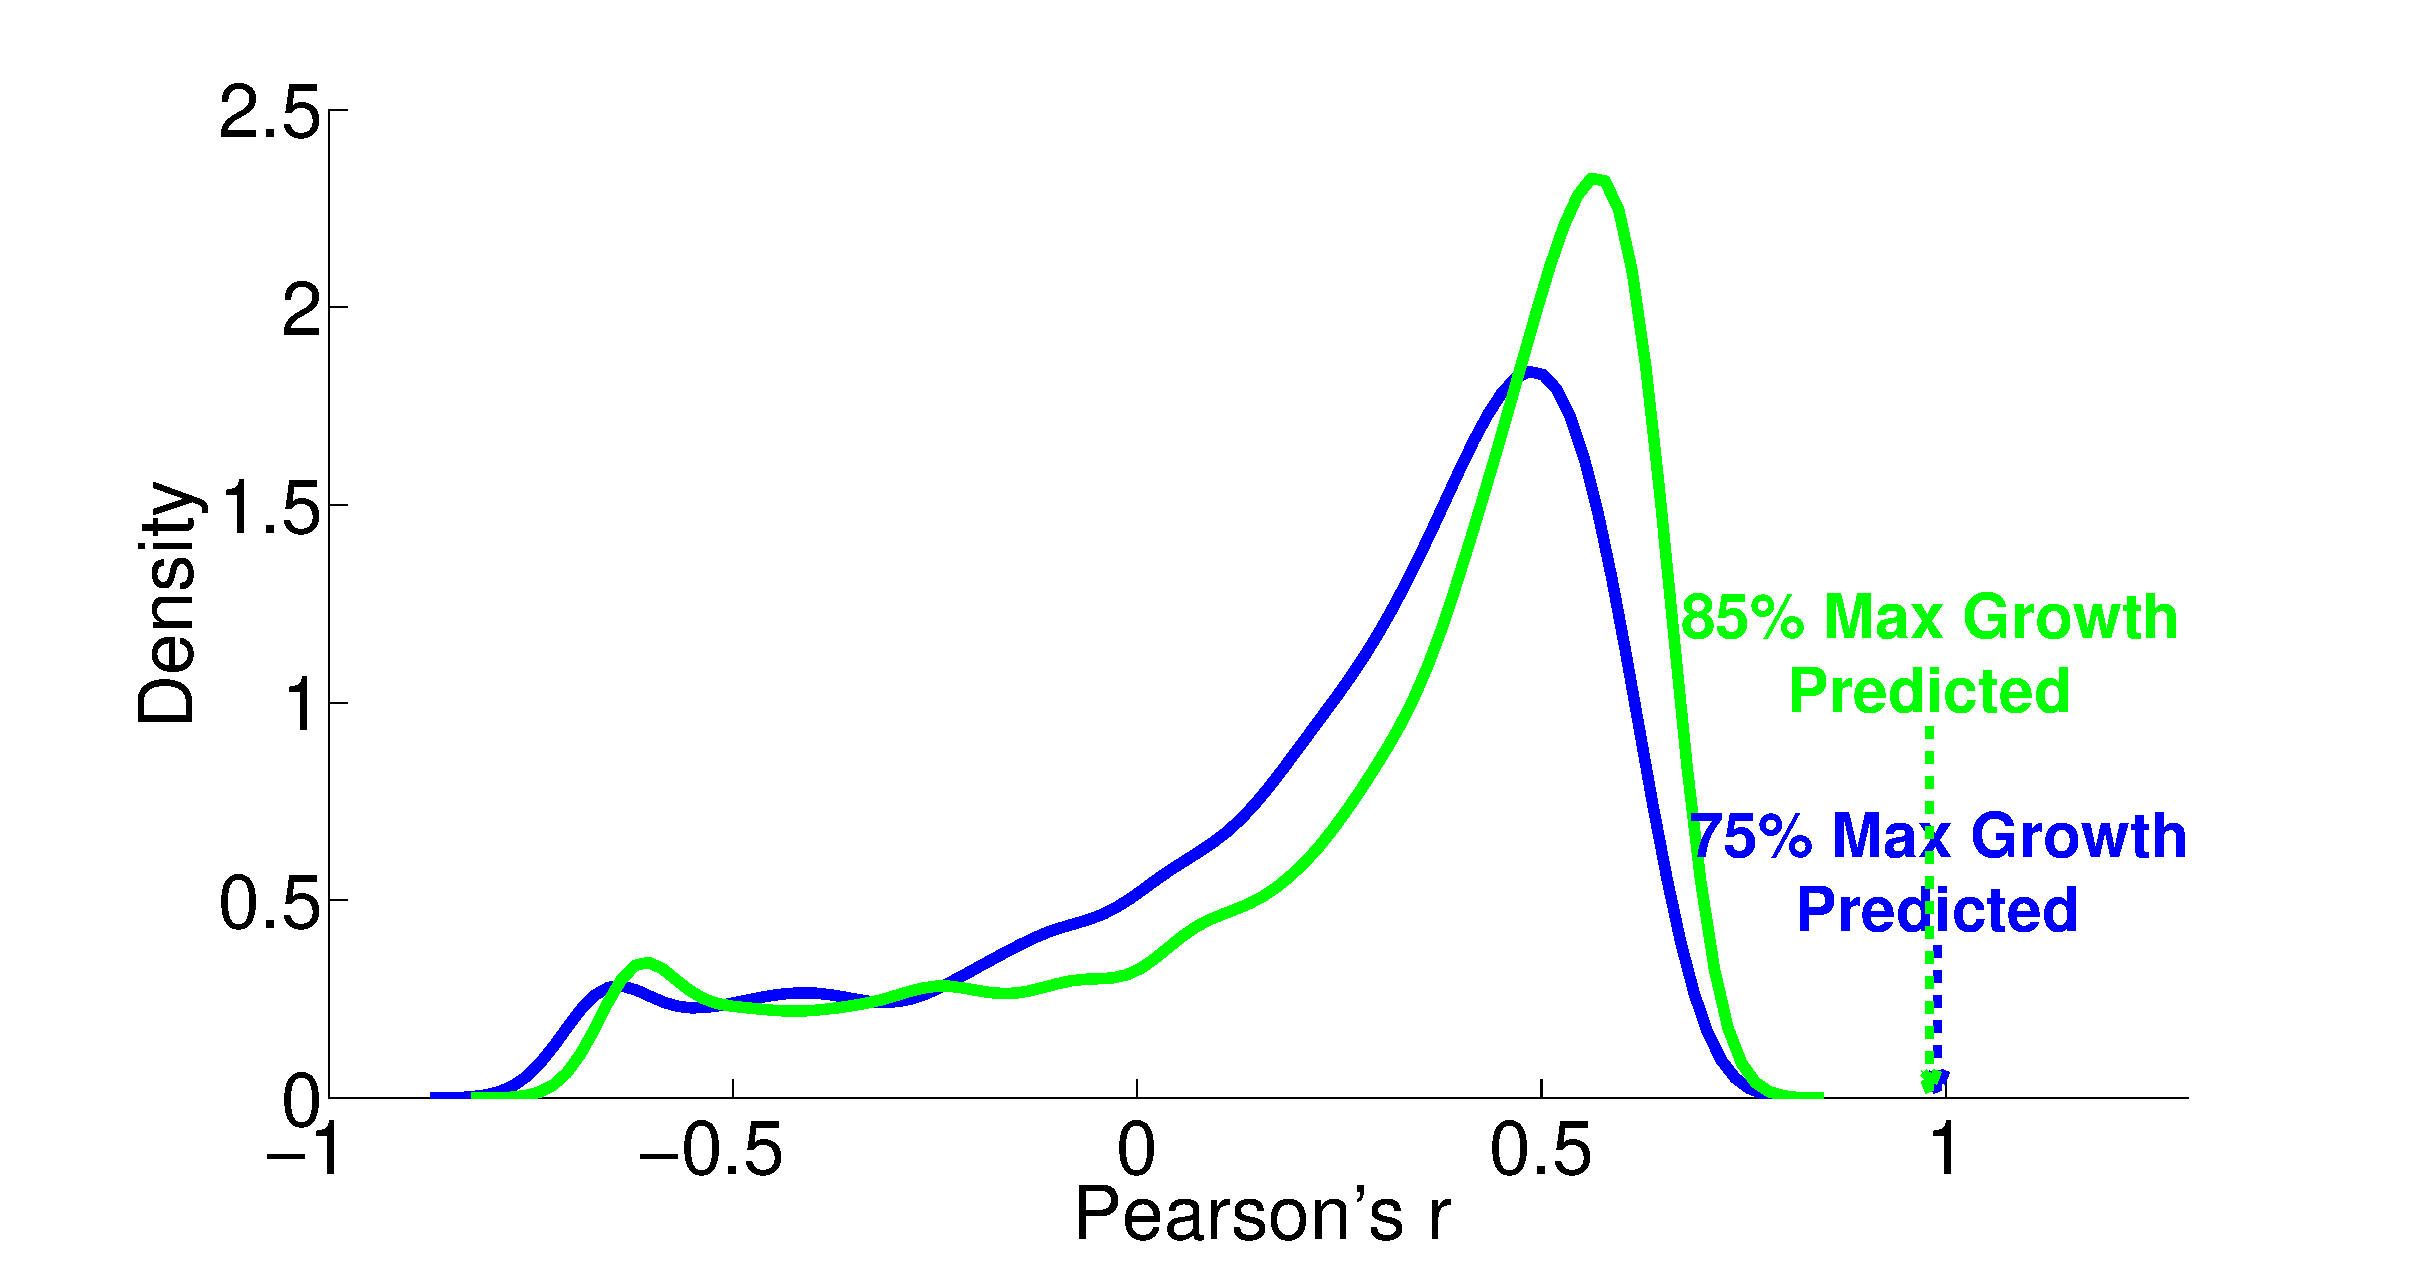
\includegraphics[width=\textwidth]{pExp}
\caption{PDFs of correlation between experimental fluxes and fluxes
estimated from FALCON when all gene expression data points are
permuted.}
\label{fig:YpermCorrH}
\end{figure}
}

%%%%%%%%%%%%%%%%%%%%%%%%%%%%%%%%%%%%%%%%%%%%%%%%%%%%%%%%%%%%%%%%%%%%%%%%%%%%%%%%%%%%%%%%%%


\frame{\frametitle{Global flux correlations from permuted inputs} 

\begin{figure}[!htb]
\centering
\begin{tabular}{cc}
  \begin{subfigure}[b]{0.5\textwidth}
  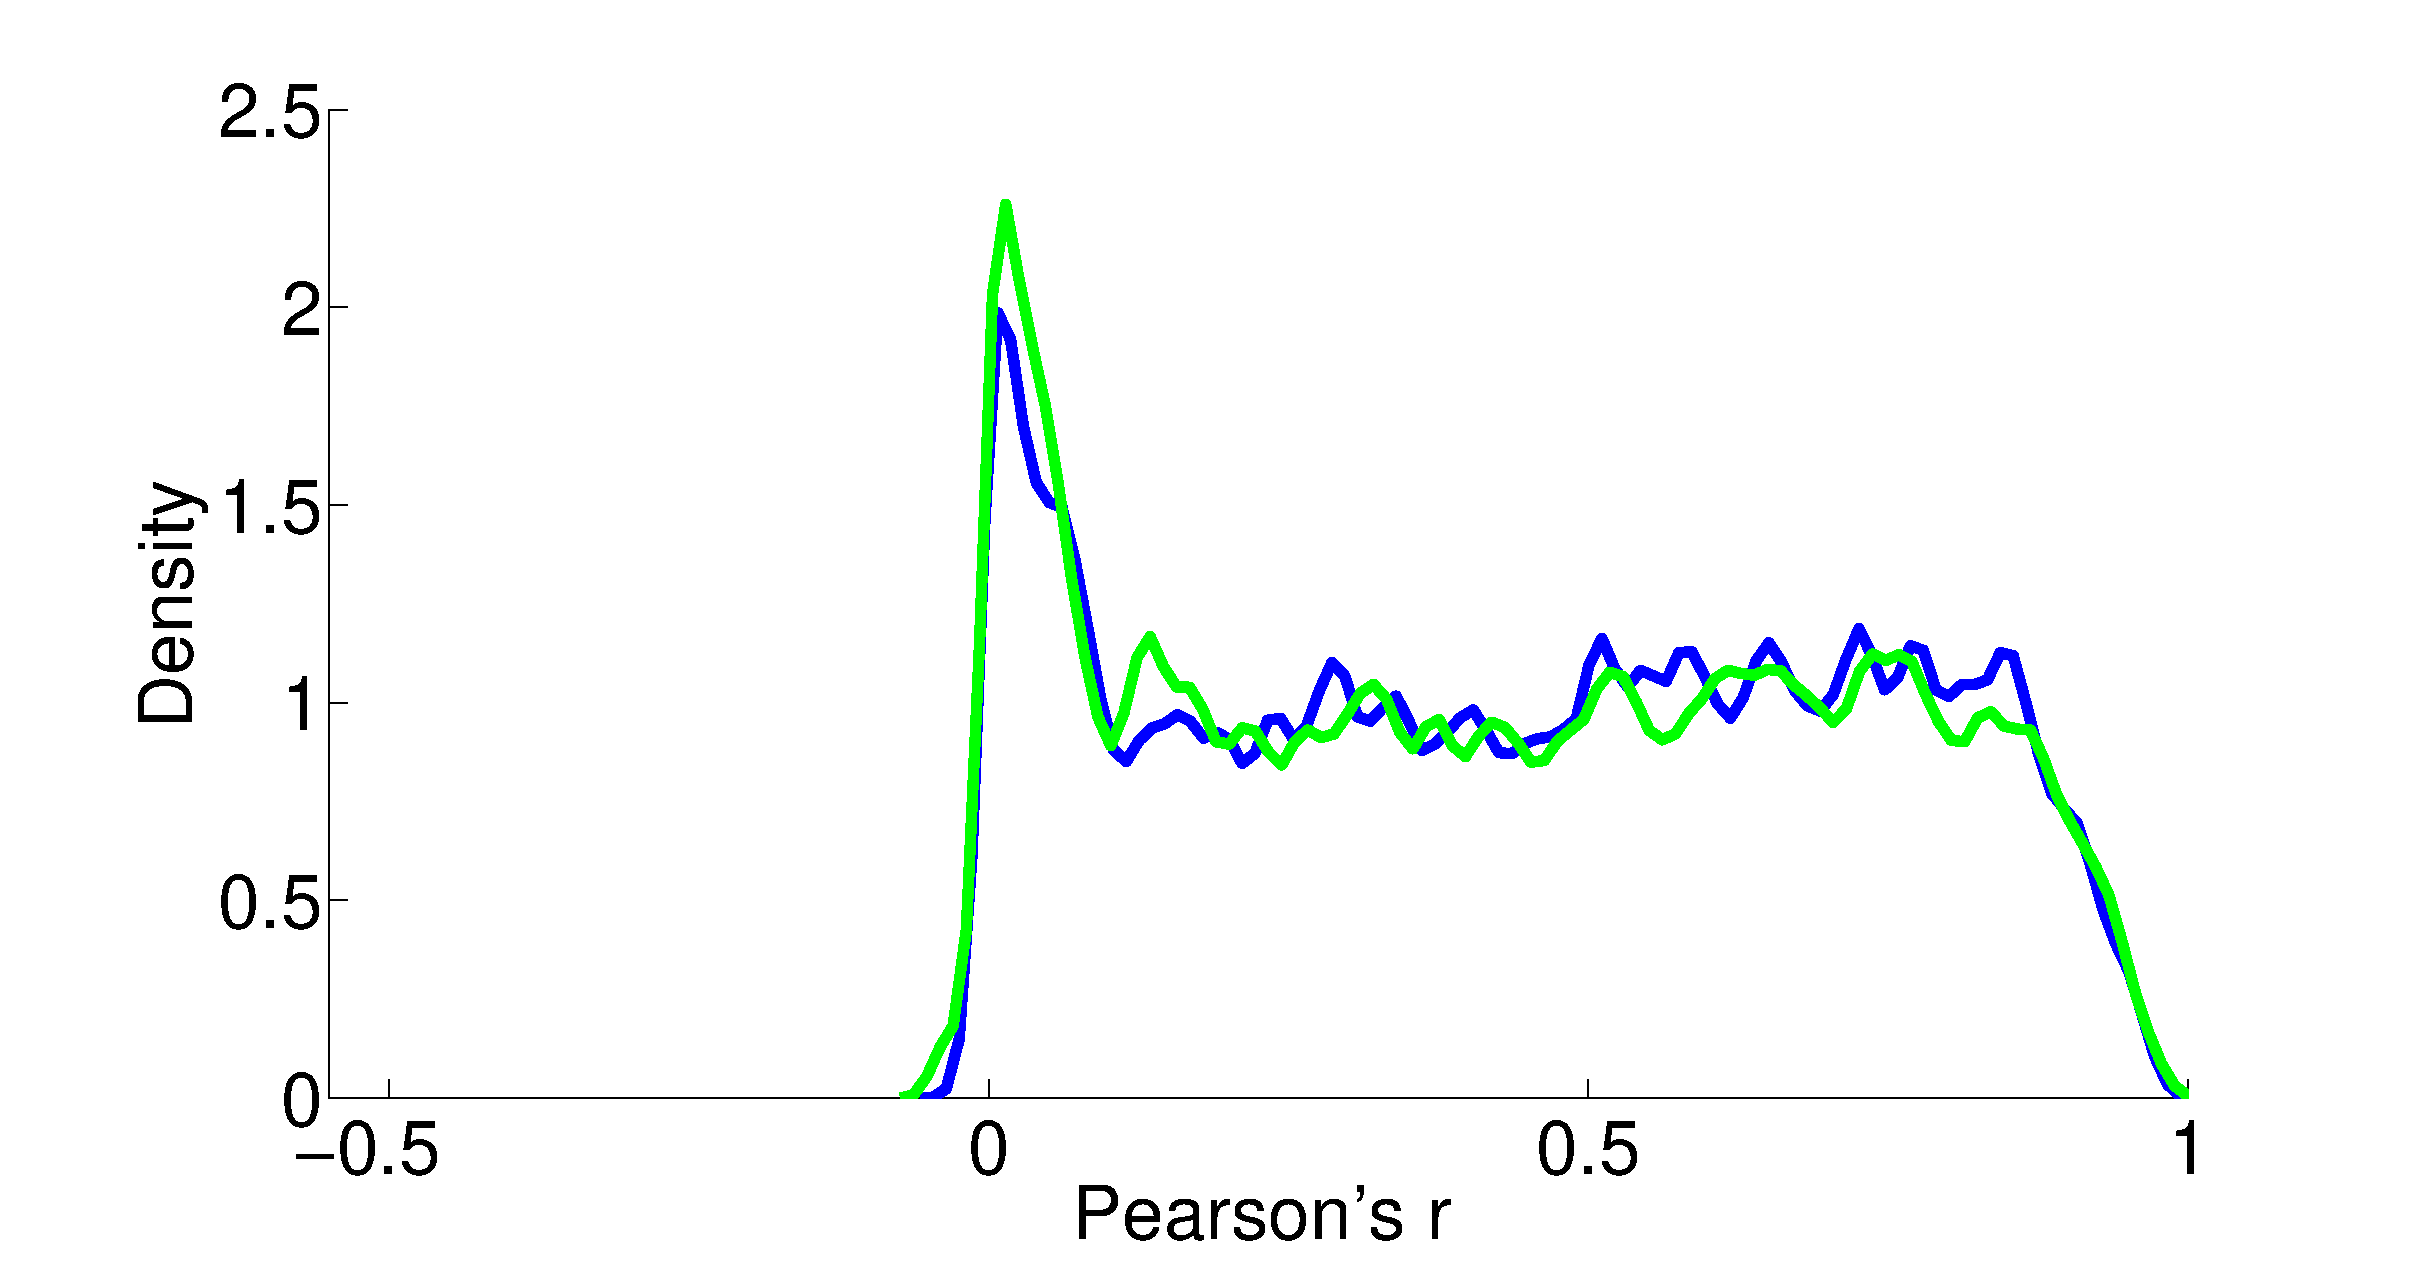
\includegraphics[width=\textwidth]{pFluxVec}
  \caption{highly constrained} \label{fig:YpermCorrSup:A}
  \end{subfigure}
&
  \begin{subfigure}[b]{0.5\textwidth}
  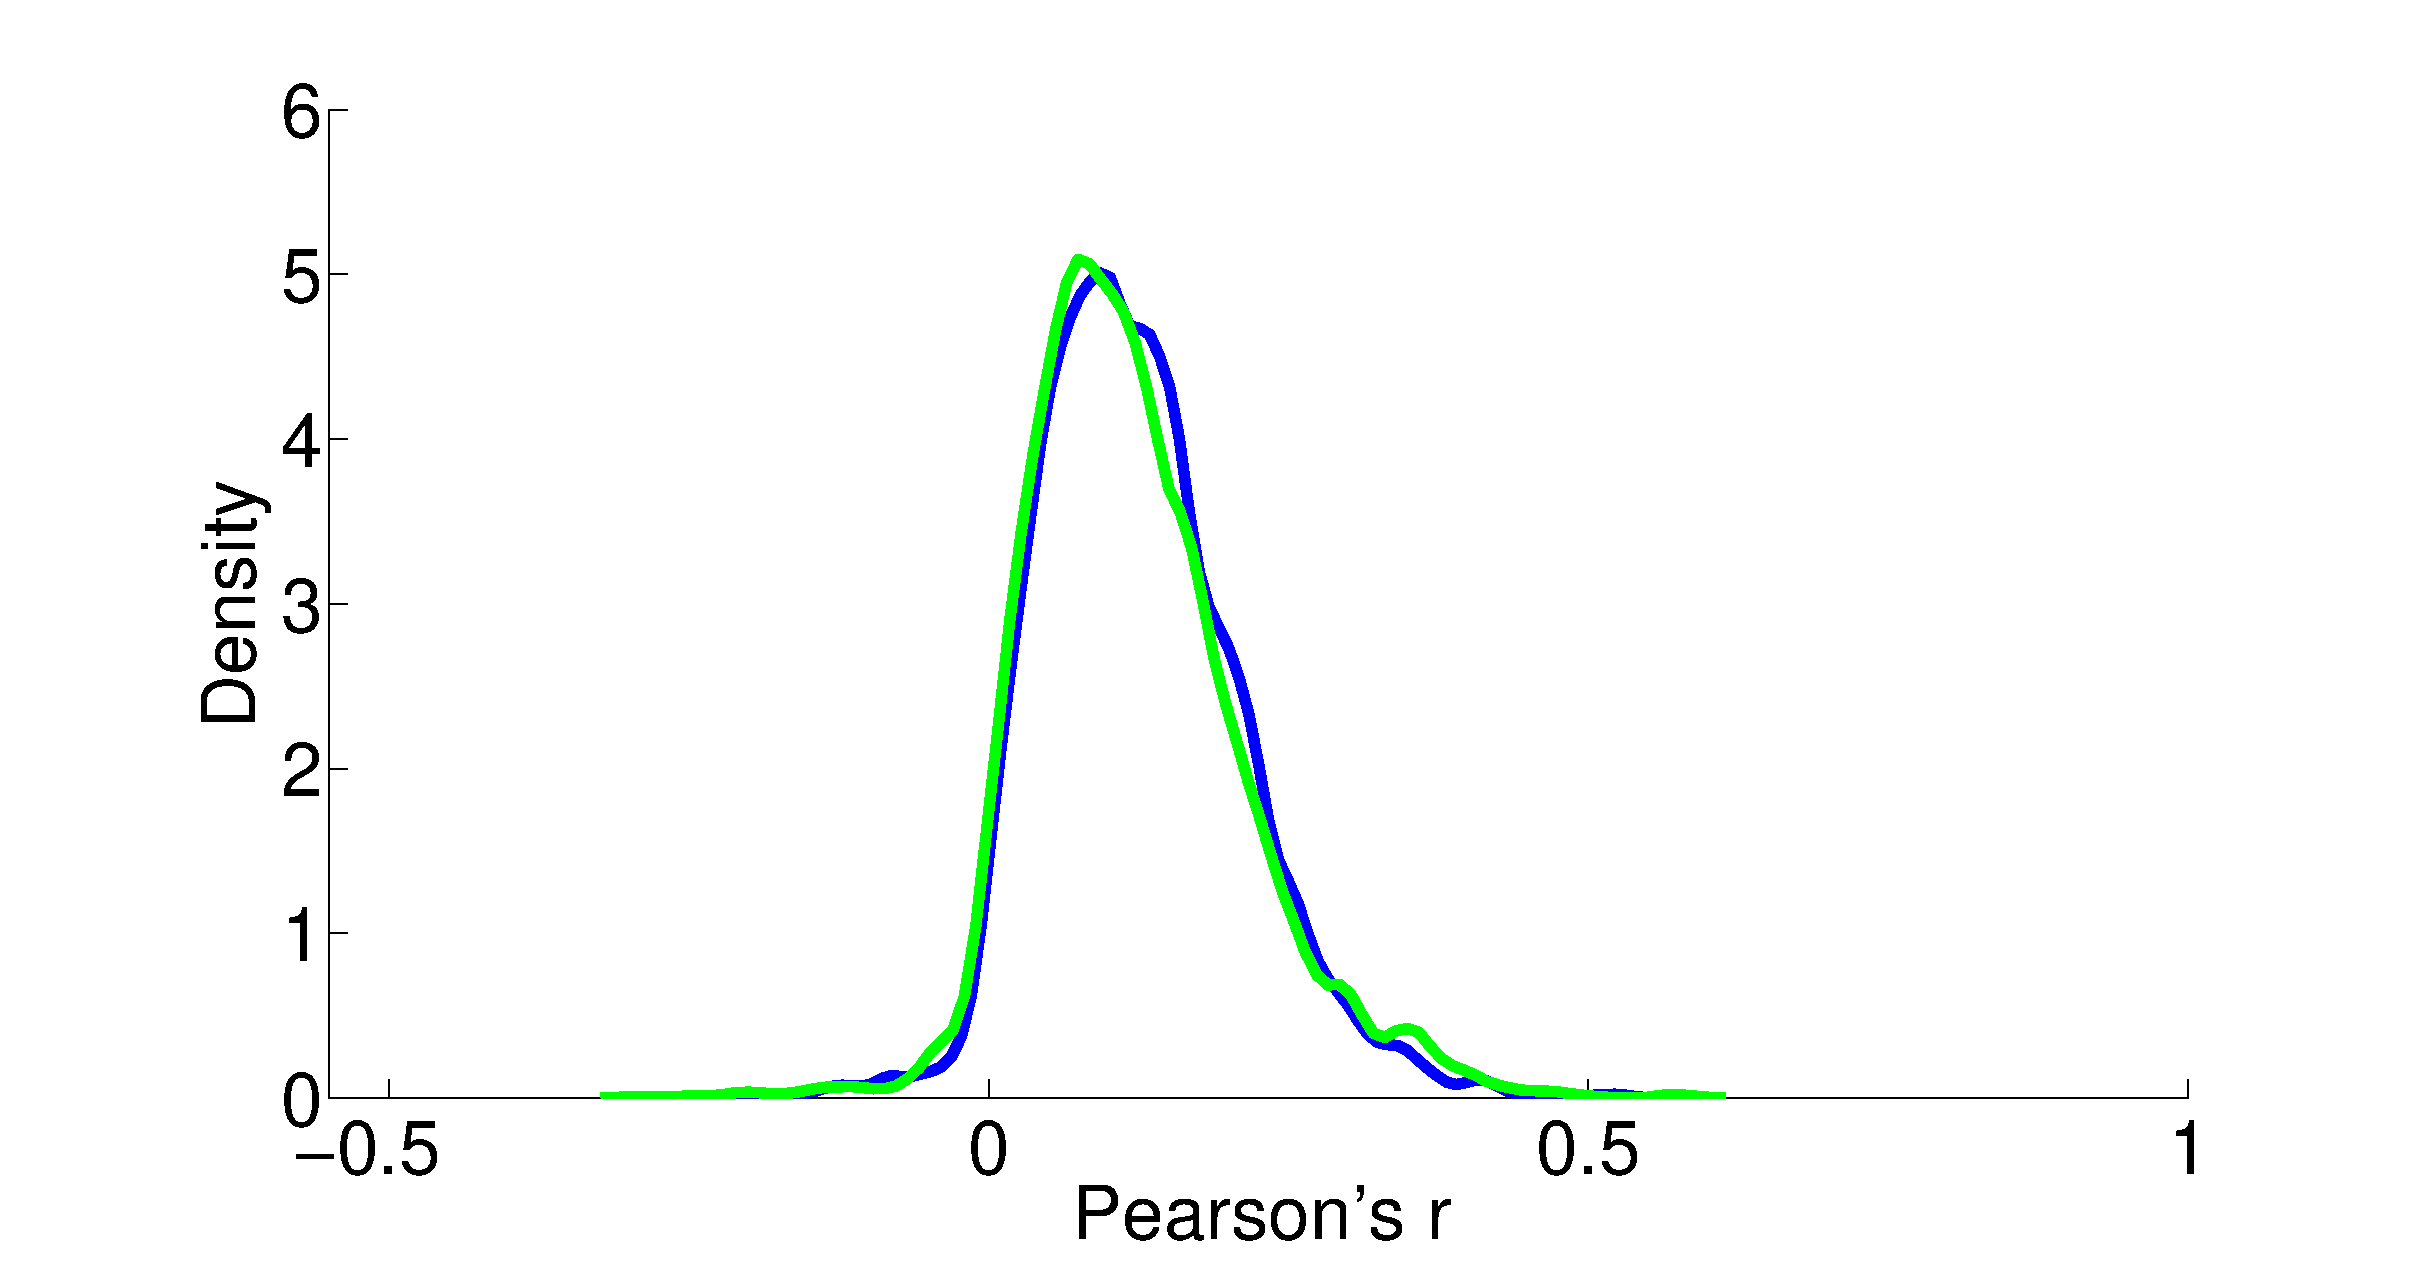
\includegraphics[width=\textwidth]{pFluxVec_dirr}
  \caption{minimally constrained} \label{fig:YpermCorrSup:B}
  \end{subfigure} 
\\
\end{tabular}
\vspace{-4mm}
\caption{PDFs of Pearson's correlation between fluxes estimated from
permuted and unpermuted complex abundance.}
\label{fig:YpermCorrSup:pearson}
\end{figure}
}

%%%%%%%%%%%%%%%%%%%%%%%%%%%%%%%%%%%%%%%%%%%%%%%%%%%%%%%%%%%%%%%%%%%%%%%%%%%%%%%%%%%%%%%%%%

\frame{\frametitle{Global flux correlations from permuted inputs} 

\begin{figure}[!htb]
\centering
\begin{tabular}{cc}
  \begin{subfigure}[b]{0.5\textwidth}
  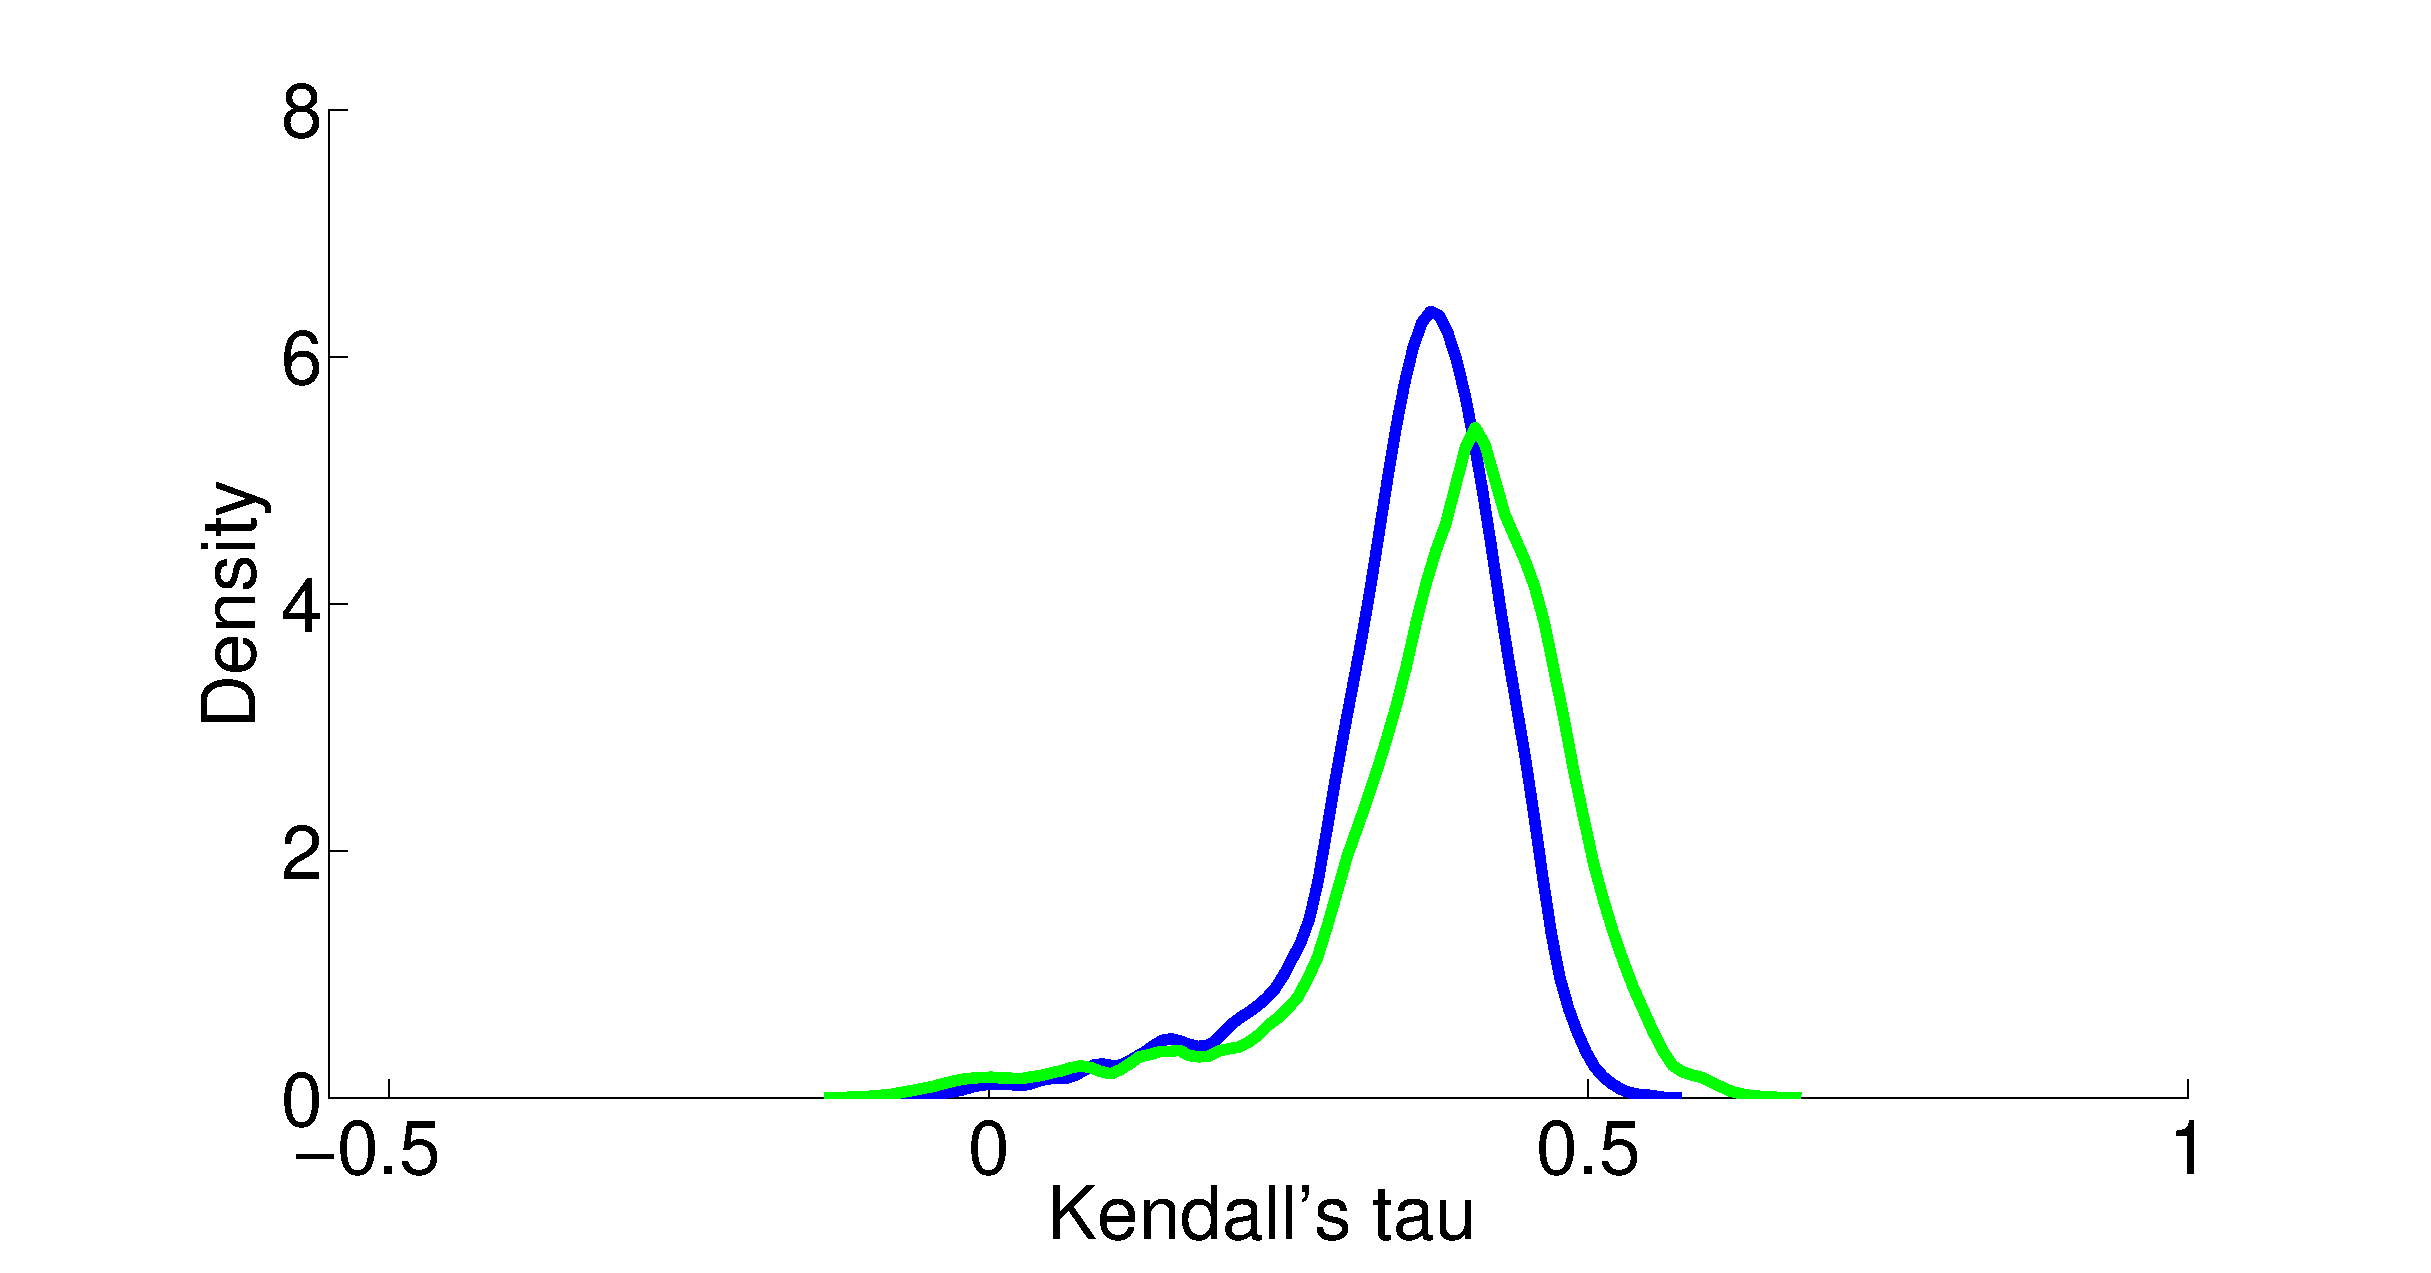
\includegraphics[width=\textwidth]{kFluxVec}
  \caption{highly constrained} \label{fig:YpermCorrSup:C}
  \end{subfigure}
&
  \begin{subfigure}[b]{0.5\textwidth}
  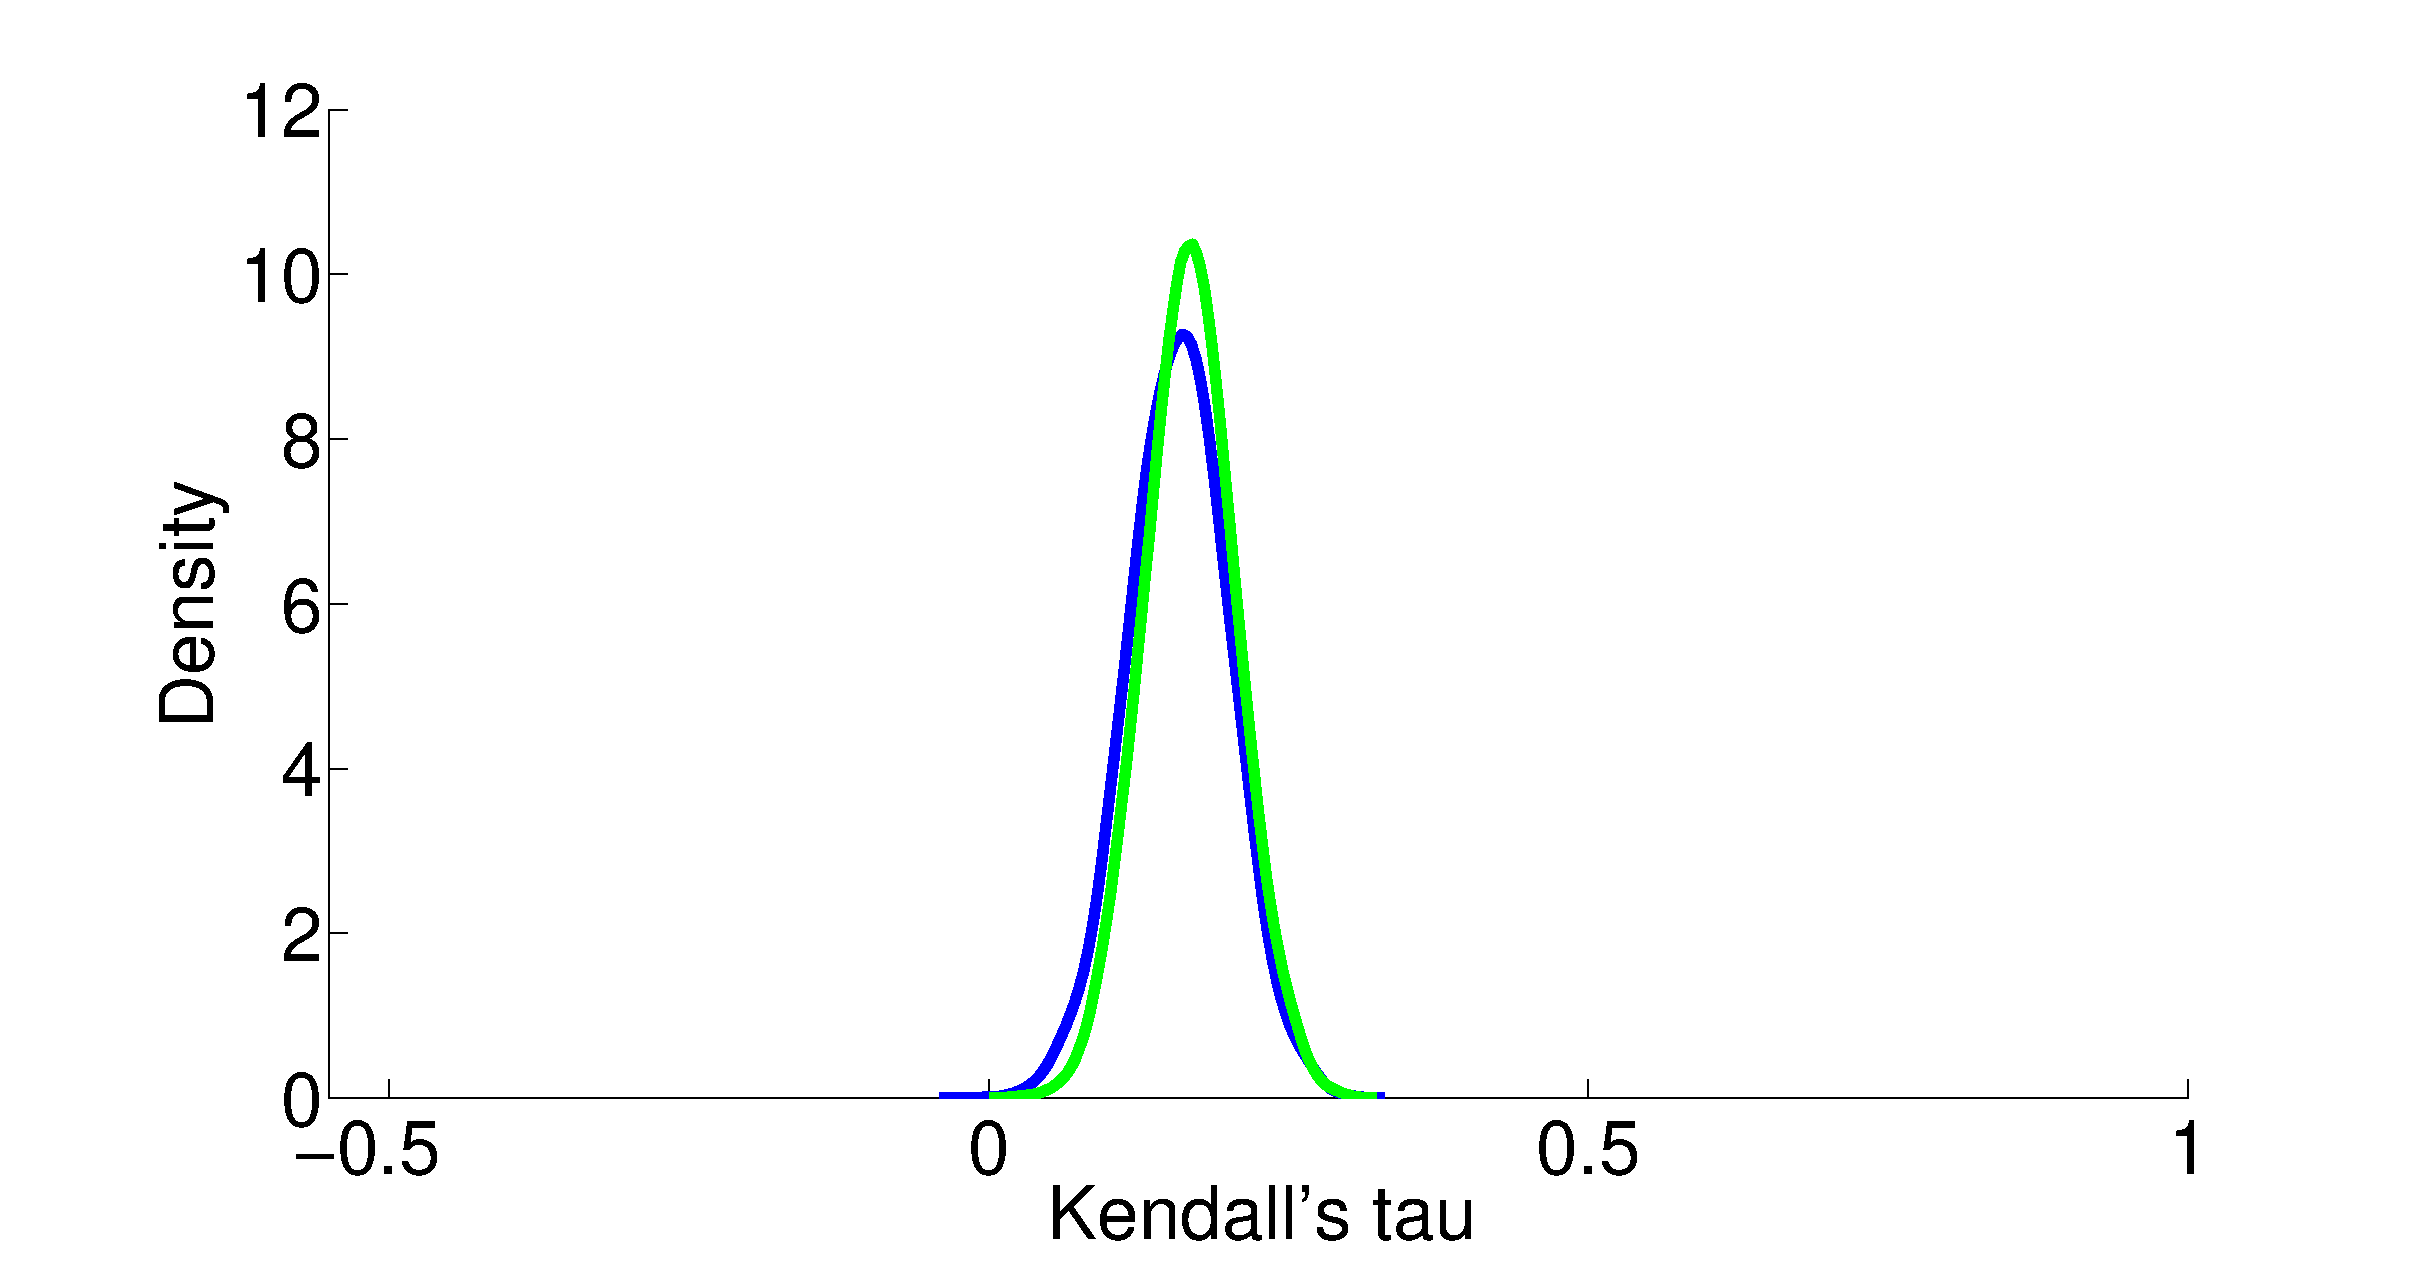
\includegraphics[width=\textwidth]{kFluxVec_dirr}
  \caption{minimally constrained} \label{fig:YpermCorrSup:D}
  \end{subfigure} 
\\
\end{tabular}
\vspace{-4mm}
\caption{PDFs of Kendall's correlation between fluxes estimated from
permuted and unpermuted complex abundance.}
\label{fig:YpermCorrSup:kendall}
\end{figure}
}

%%%%%%%%%%%%%%%%%%%%%%%%%%%%%%%%%%%%%%%%%%%%%%%%%%%%%%%%%%%%%%%%%%%%%%%%%%%%%%%%%%%%%%%%%%

\frame{\frametitle{Correlation of perturbed inputs (complex abundance)} 

\begin{figure}
\centering
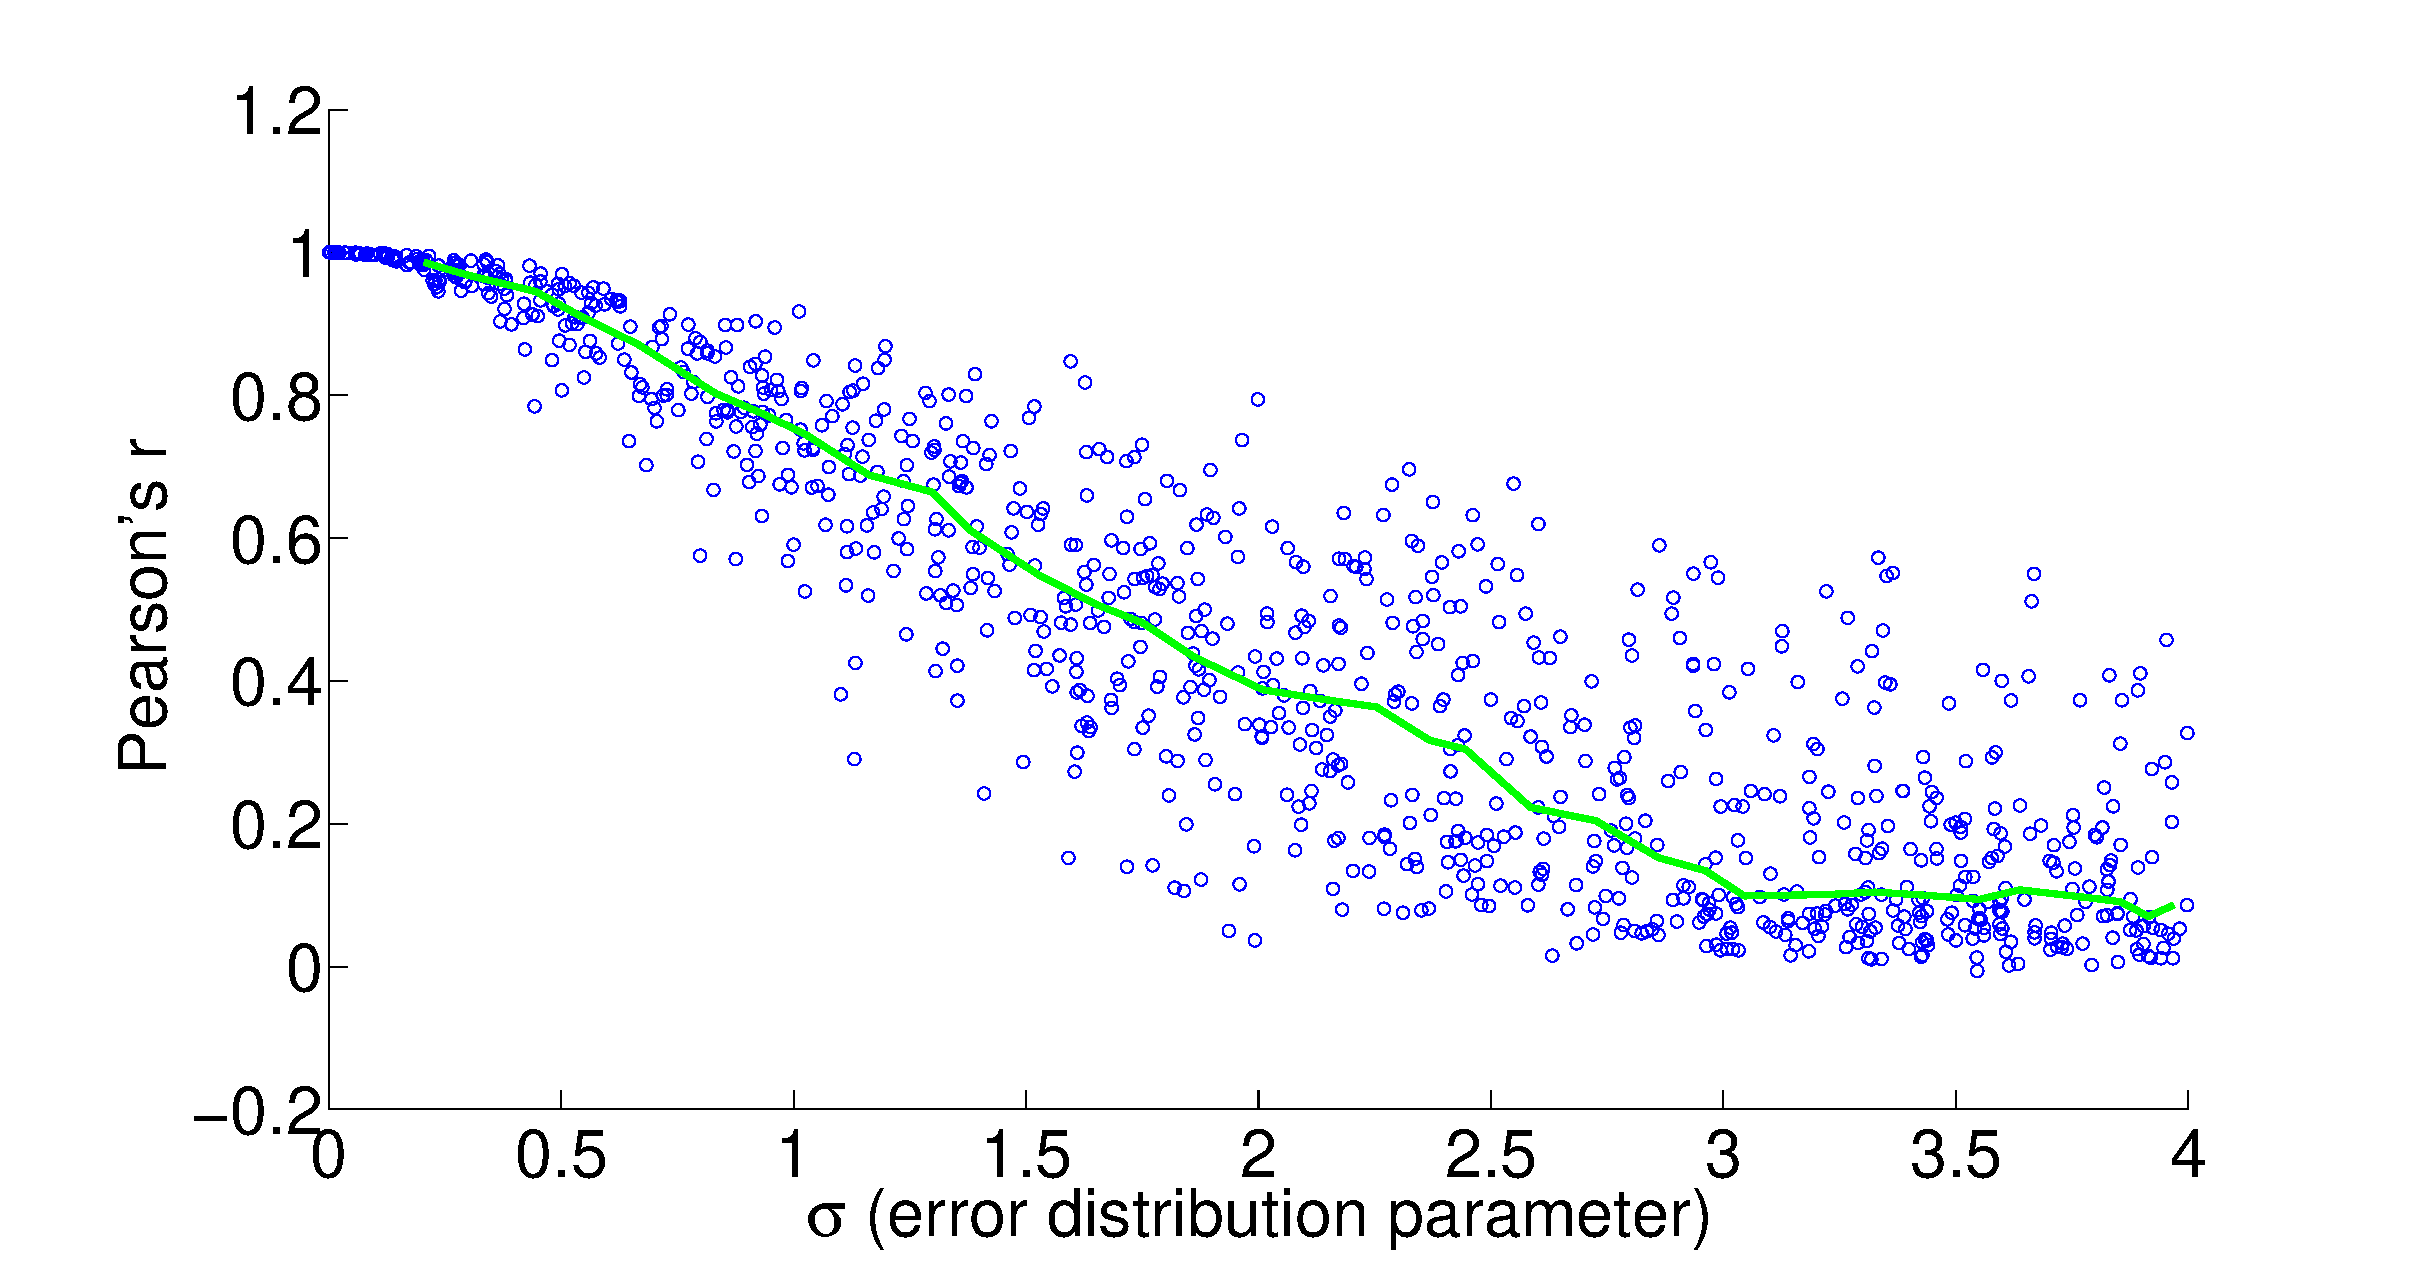
\includegraphics[width=\textwidth]{noise_y7EC}
\caption{Correlation of perturbed enzyme abundance vectors with the
associated unperturbed vector for the Yeast~7 model.}
\label{fig:ExpSens:Complex}
\end{figure}

}

%%%%%%%%%%%%%%%%%%%%%%%%%%%%%%%%%%%%%%%%%%%%%%%%%%%%%%%%%%%%%%%%%%%%%%%%%%%%%%%%%%%%%%%%%%

\frame{\frametitle{Method comparison for enzyme complex quantification}
\framesubtitle{The effect on FALCON-estimated fluxes in Yeast} 

\begin{figure}
\centering
\begin{tabular}{cc}
  \begin{subfigure}[b]{0.5\textwidth}
  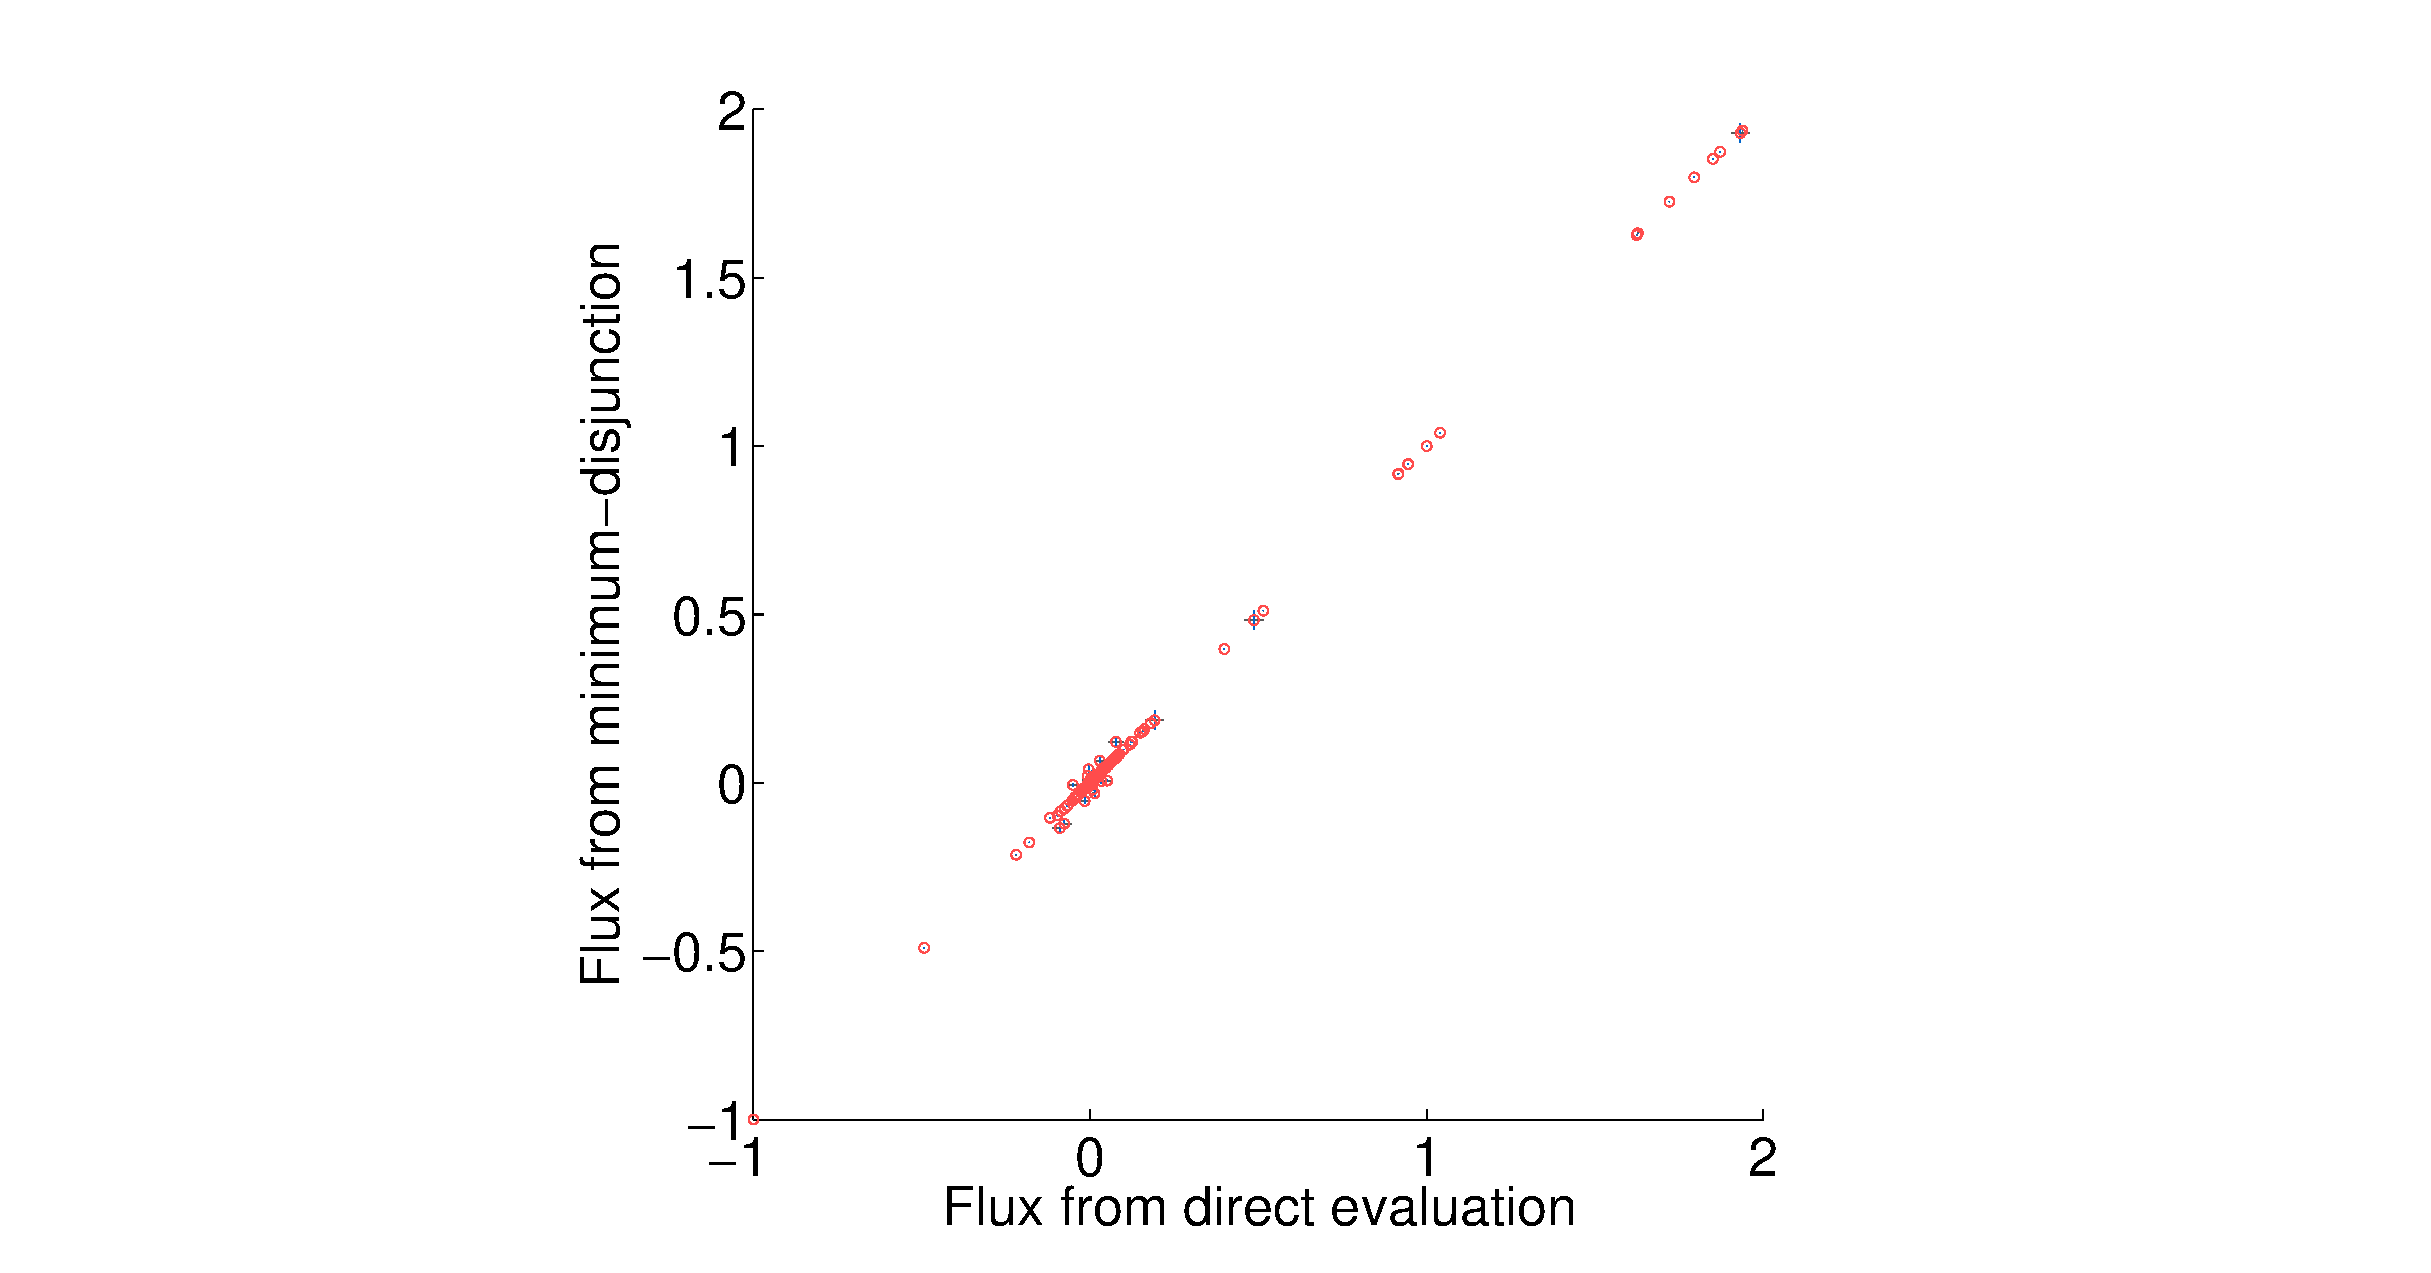
\includegraphics[width=\textwidth, trim=9cm 0cm 9cm 0cm, clip=true]
  {expCmpY7HC}
  \caption{highly constrained}
  \end{subfigure} 
&
  \begin{subfigure}[b]{0.5\textwidth}
  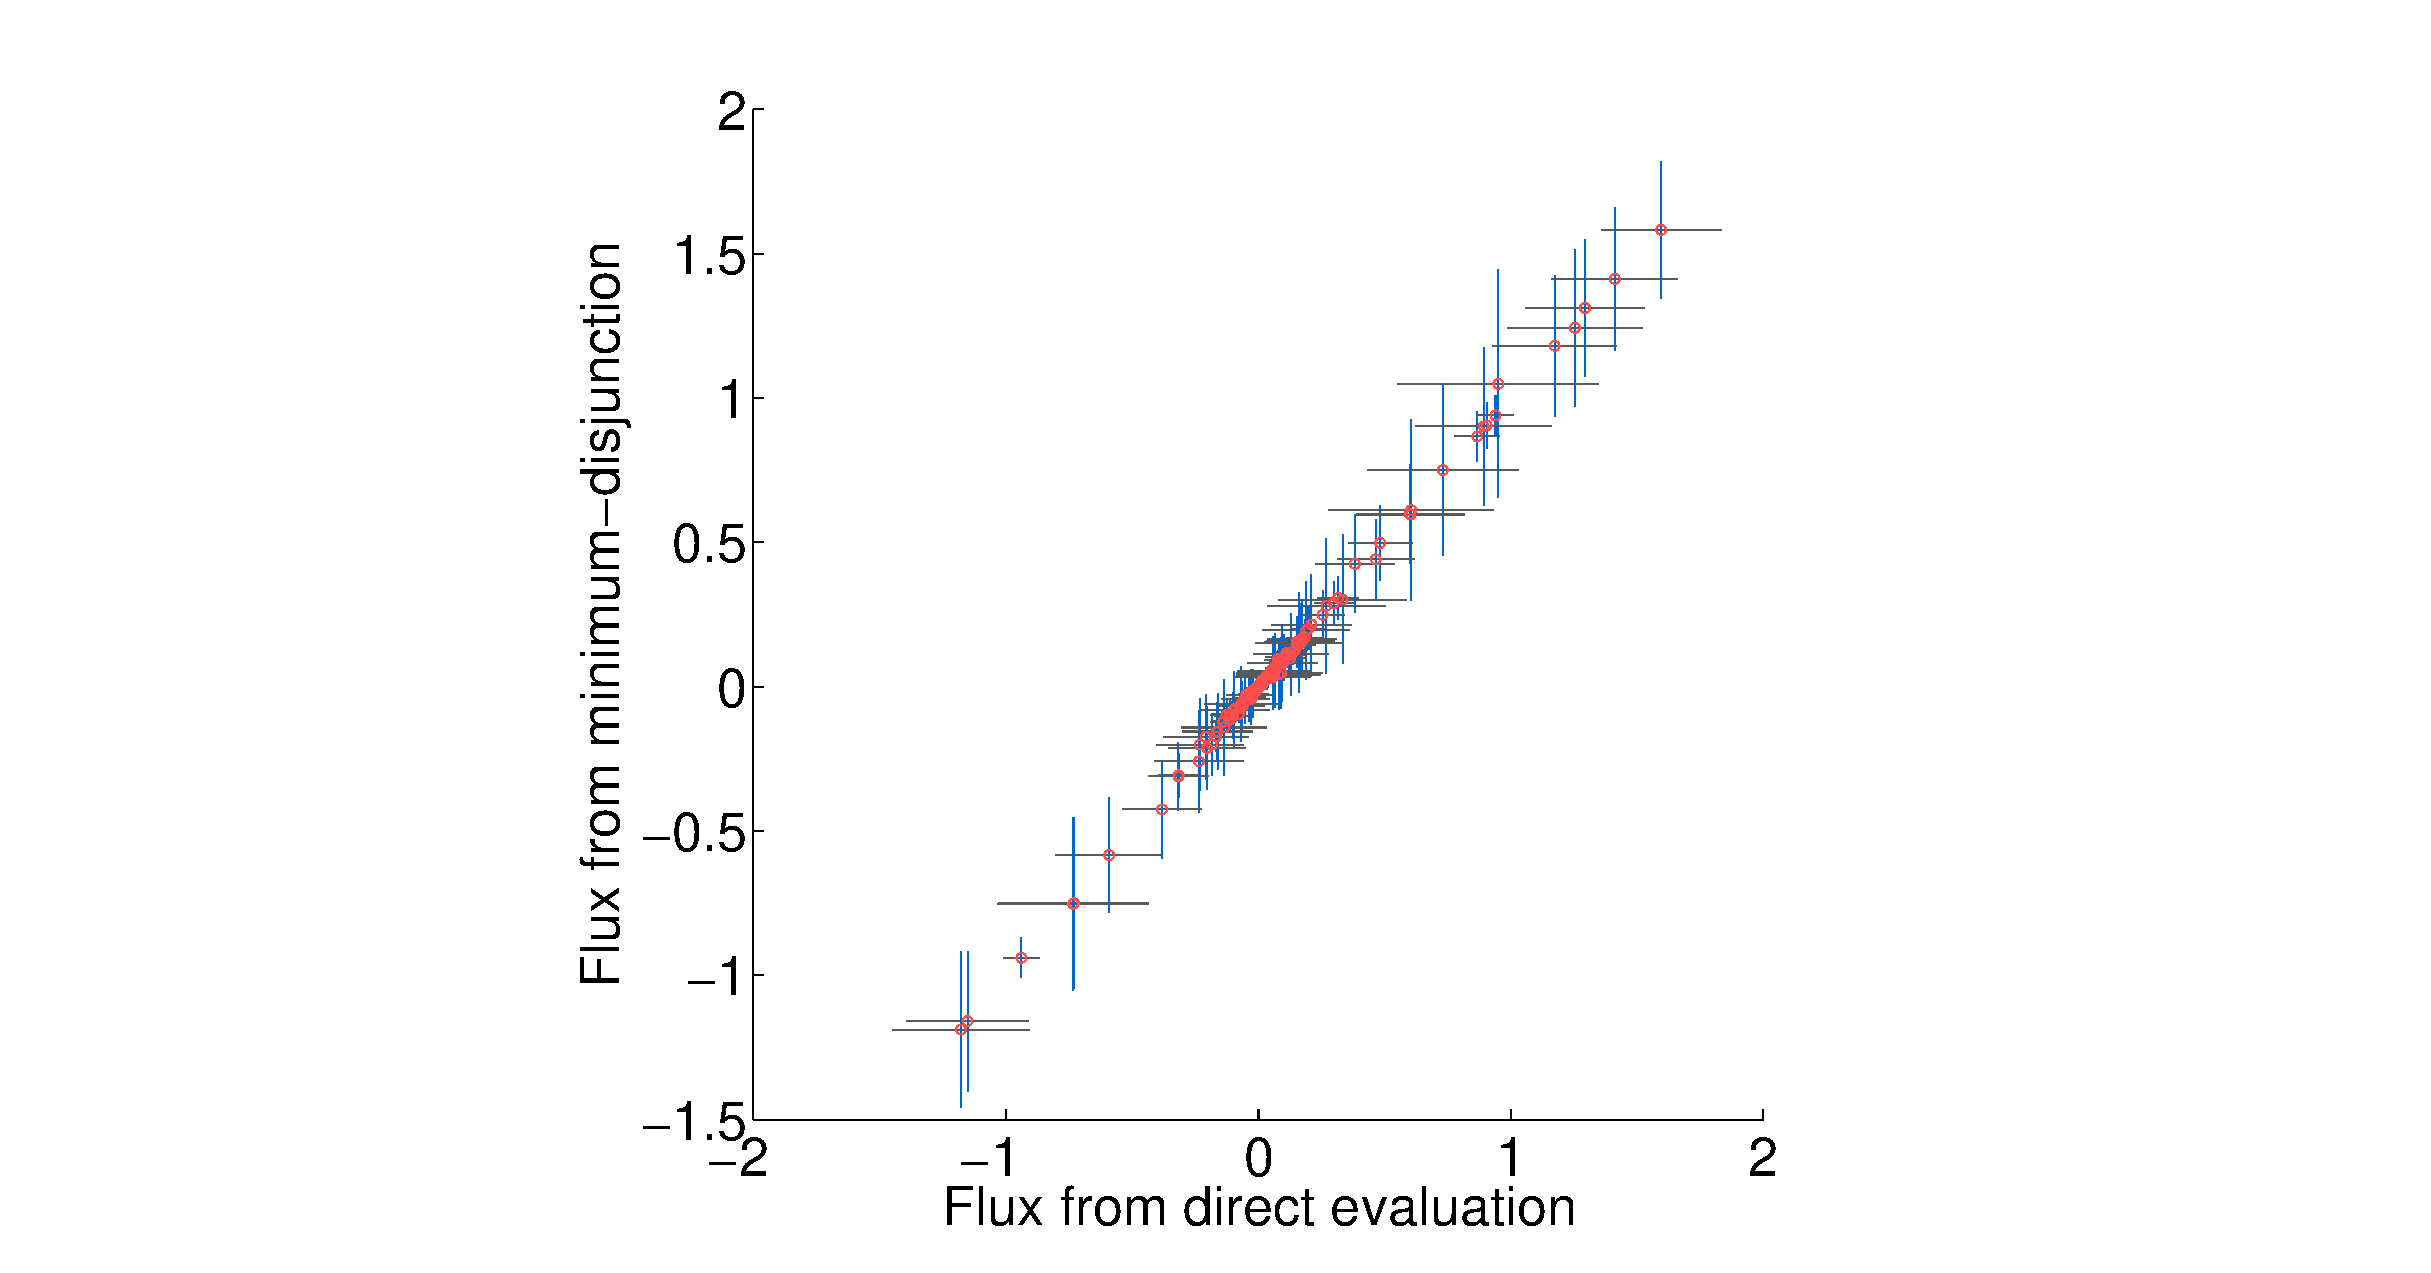
\includegraphics[width=\textwidth, trim=9cm 0cm 9cm 0cm, clip=true]
  {expCmpY7MC}
  \caption{minimally constrained}
  \end{subfigure} 
\\
\end{tabular}
\vspace{-4mm}
\label{fig:EnzAbundEvalYCmp}
\end{figure}
}

\note{
Relaxing constraints imposes no major difference other than slightly 
increasing the error in yeast model.
\par}

%%%%%%%%%%%%%%%%%%%%%%%%%%%%%%%%%%%%%%%%%%%%%%%%%%%%%%%%%%%%%%%%%%%%%%%%%%%%%%%%%%%%%%%%%%

\frame{\frametitle{Method comparison for enzyme complex quantification}
\framesubtitle{The effect on FALCON-estimated fluxes in Human} 

\begin{figure}
\centering
\begin{tabular}{cc}
  \begin{subfigure}[b]{0.5\textwidth}
  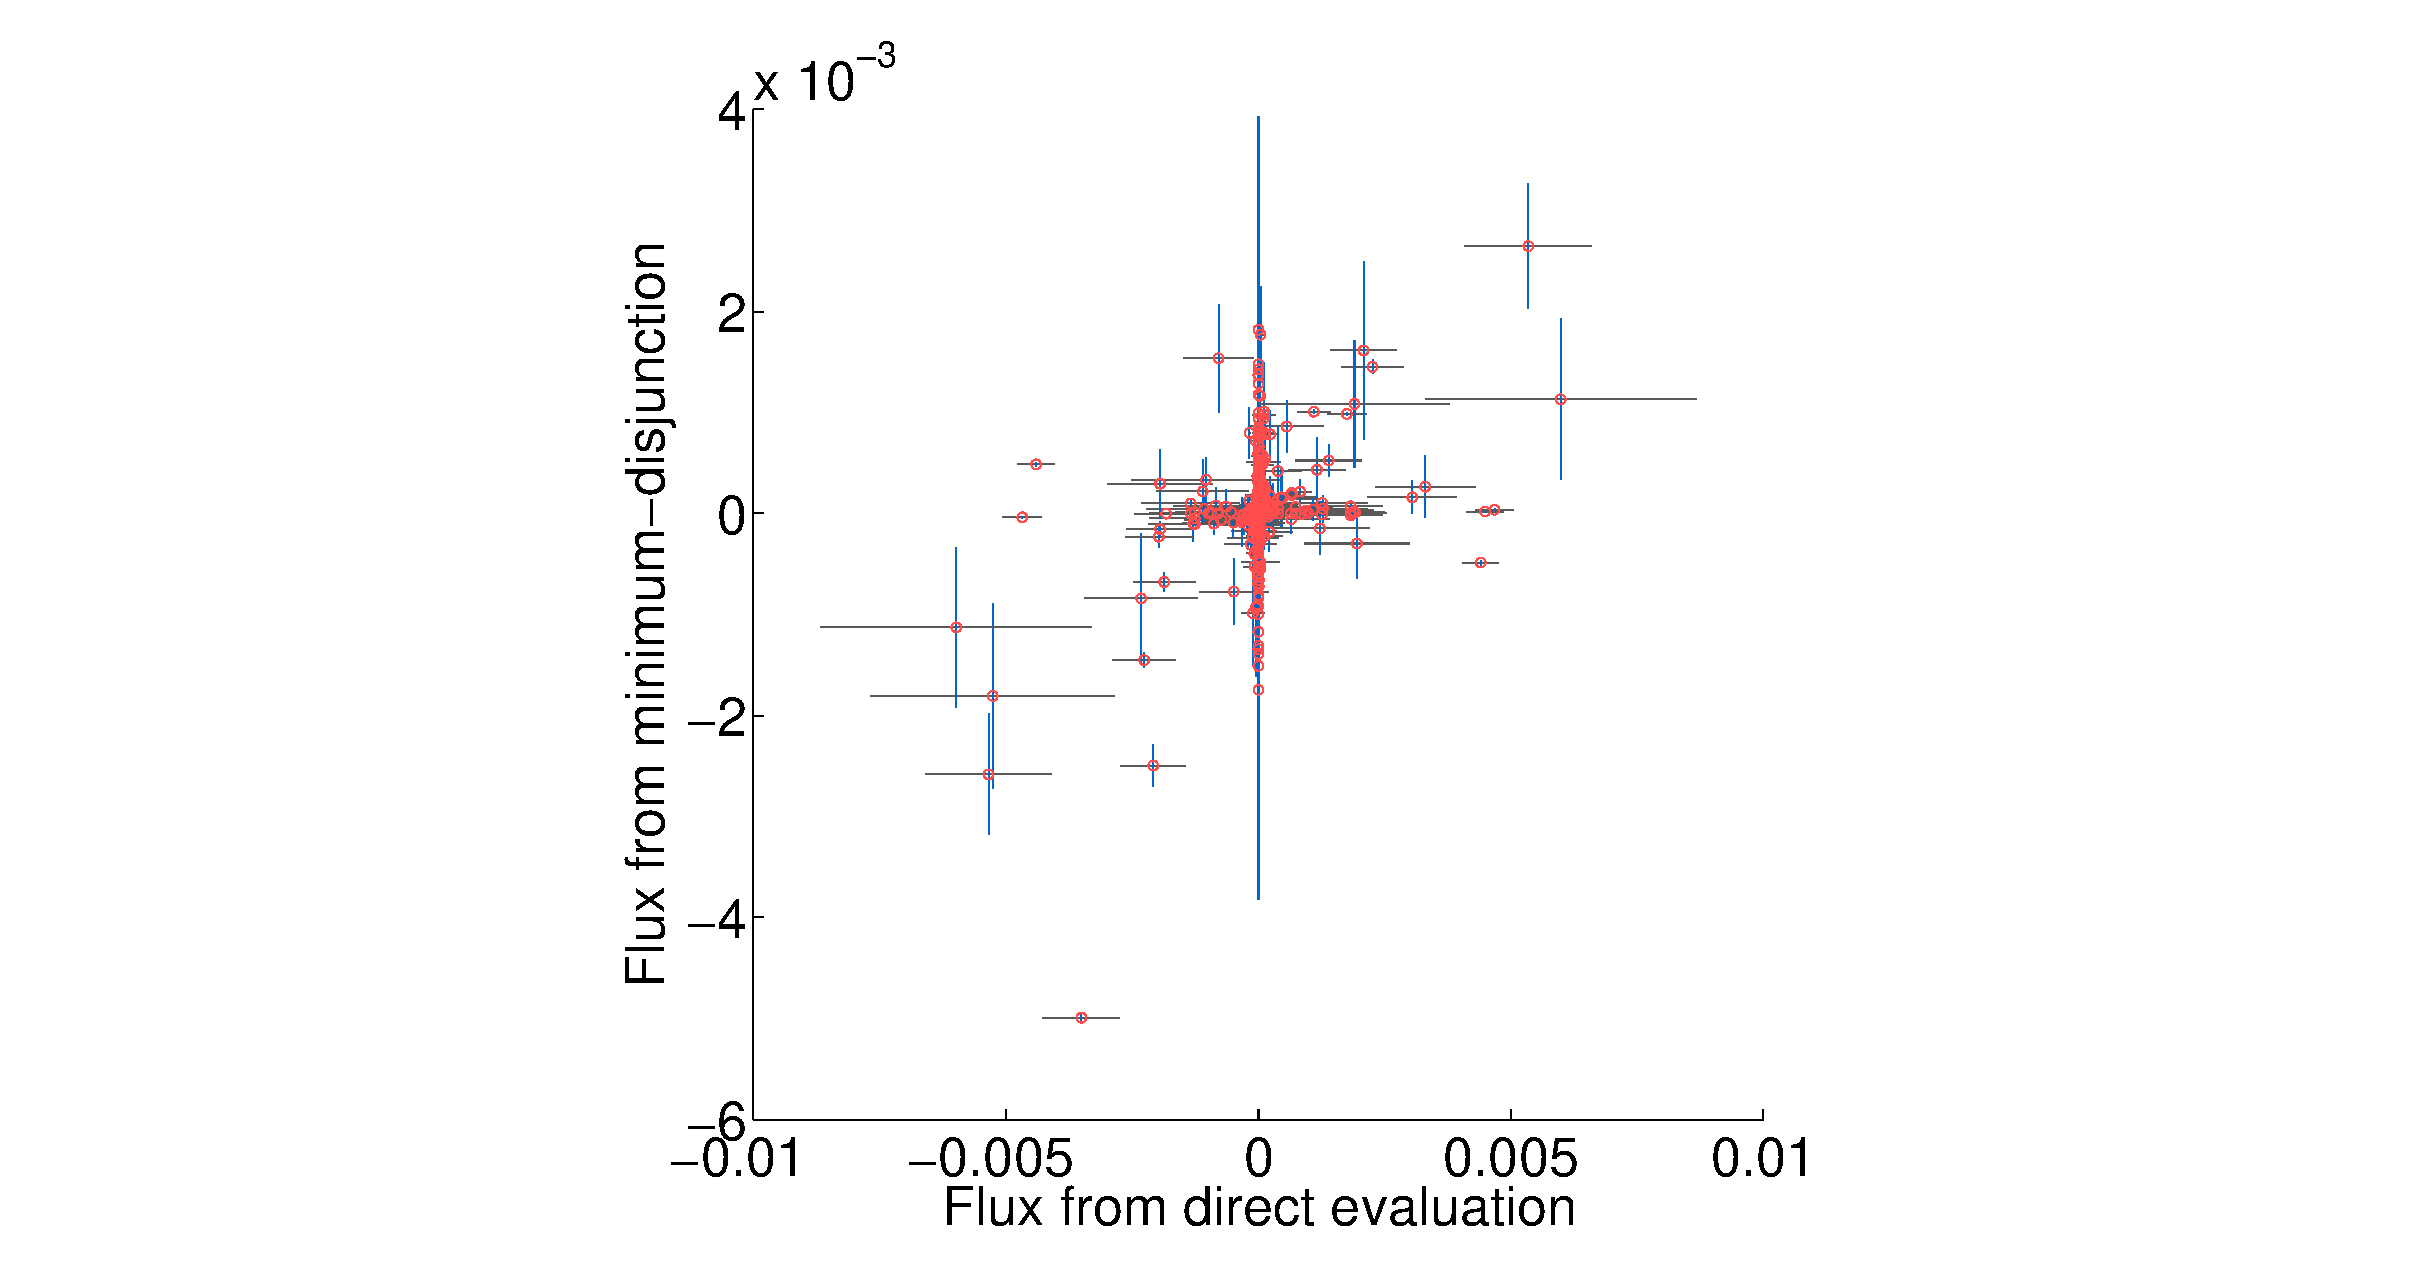
\includegraphics[width=\textwidth, trim=9cm 0cm 9cm 0cm, clip=true]
  {expCmpR2HC}
  \caption{highly constrained}
  \end{subfigure} 
&
  \begin{subfigure}[b]{0.5\textwidth}
  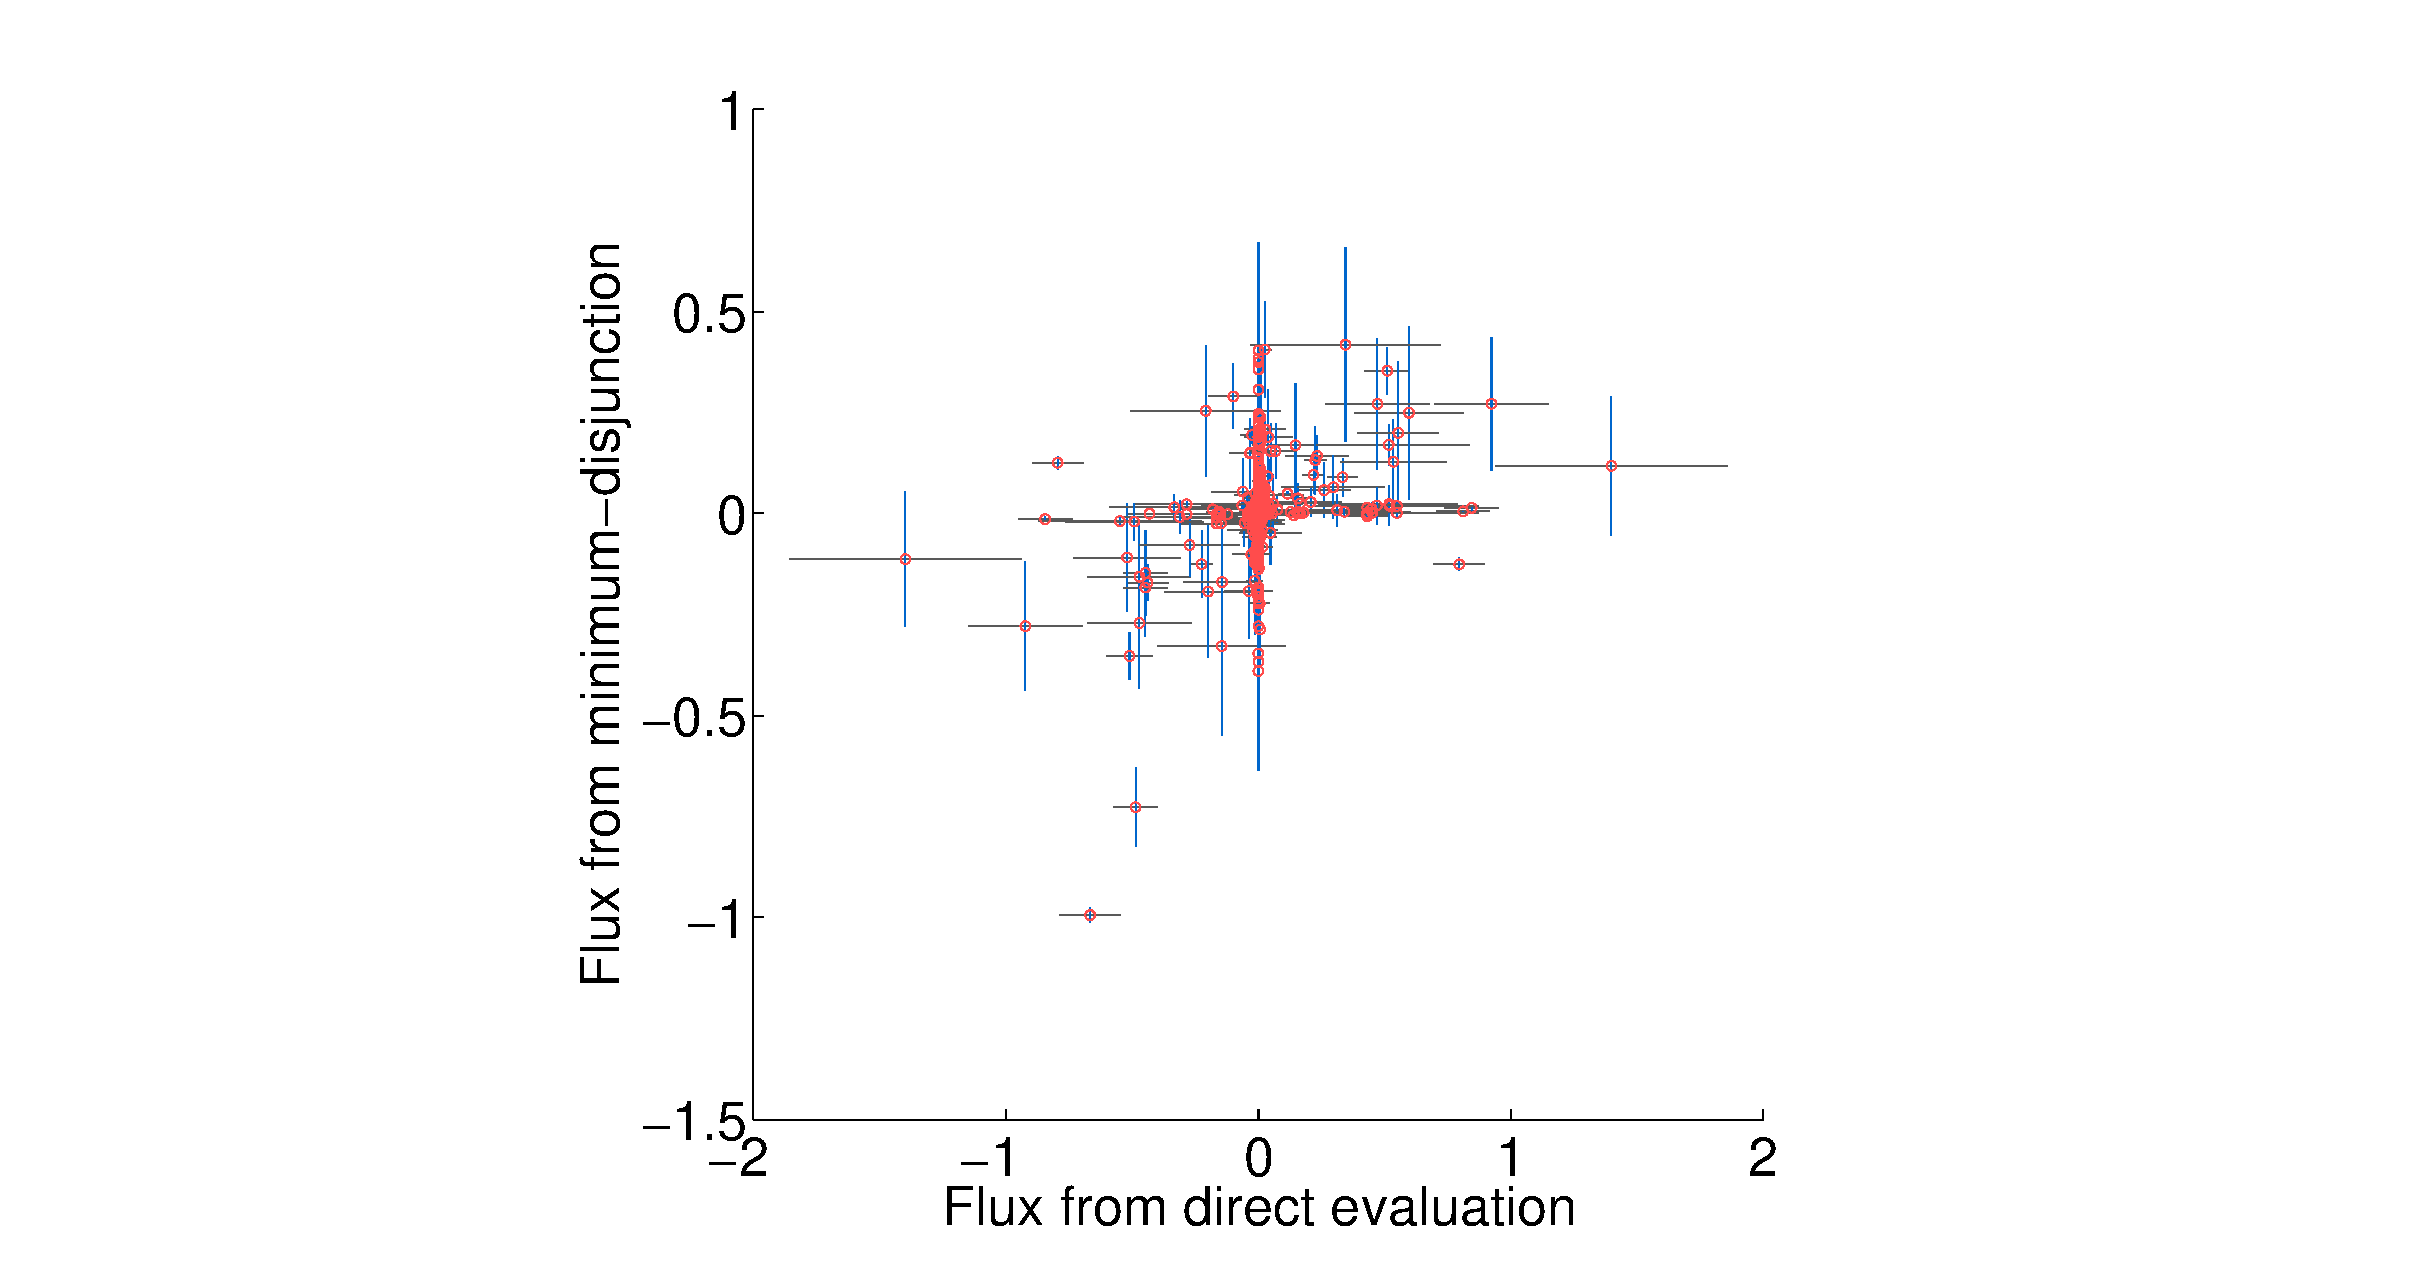
\includegraphics[width=\textwidth, trim=9cm 0cm 9cm 0cm, clip=true]
  {expCmpR2dC}
  \caption{minimally constrained}
  \end{subfigure} 
\\
\end{tabular}
\vspace{-4mm}
\label{fig:EnzAbundEvalYCmp}
\end{figure}
}

\note{
The human model is sensitive to the change in constraints when different
methods are used for enzyme-complex quantification.
\par}

%%%%%%%%%%%%%%%%%%%%%%%%%%%%%%%%%%%%%%%%%%%%%%%%%%%%%%%%%%%%%%%%%%%%%%%%%%%%%%%%%%%%%%%%%%


\frame{\frametitle{Flux estimates give us more than just complex abundance} 

\begin{figure}
\begin{tabular}{cc}
  \begin{subfigure}[b]{0.5\textwidth}   % l   b   r   t
  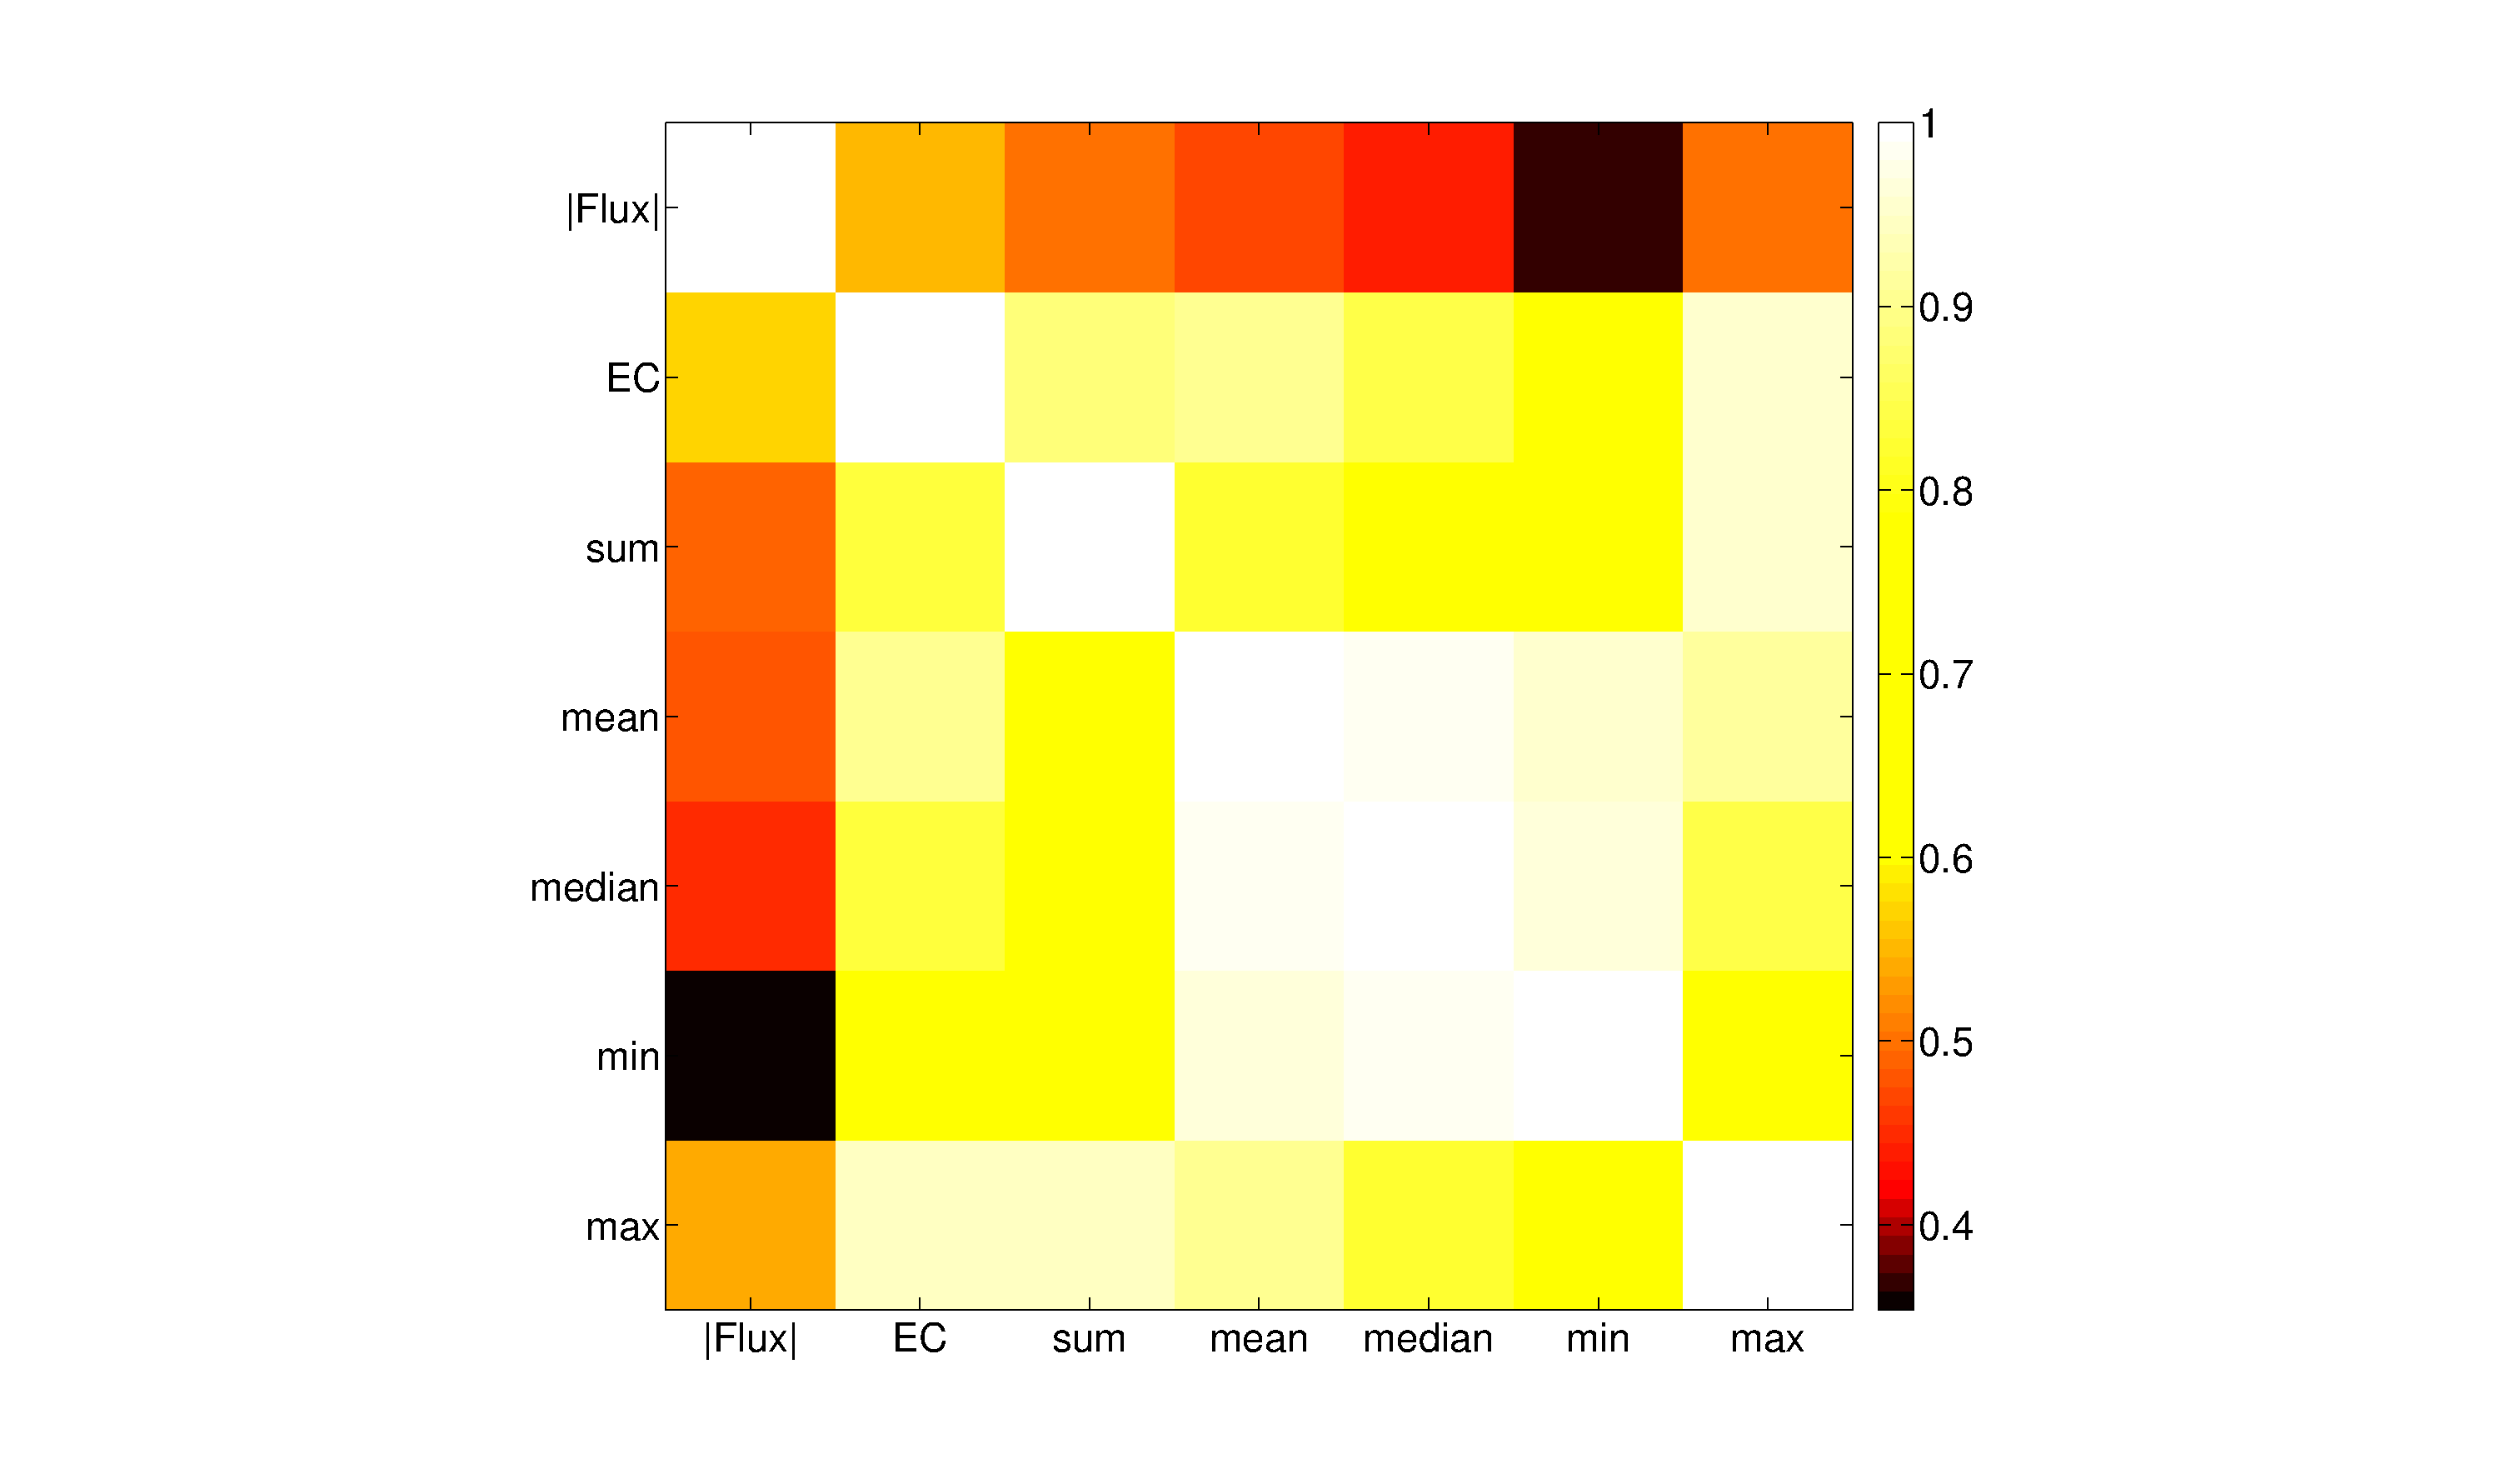
\includegraphics[width=\textwidth, trim=9cm 1.2cm 9cm 1cm, clip=true]
    {YeastExpFluxCompare}
  \caption{yeast} \label{fig:FluxExpCmp:A}
  \end{subfigure}
&
  \begin{subfigure}[b]{0.5\textwidth}
  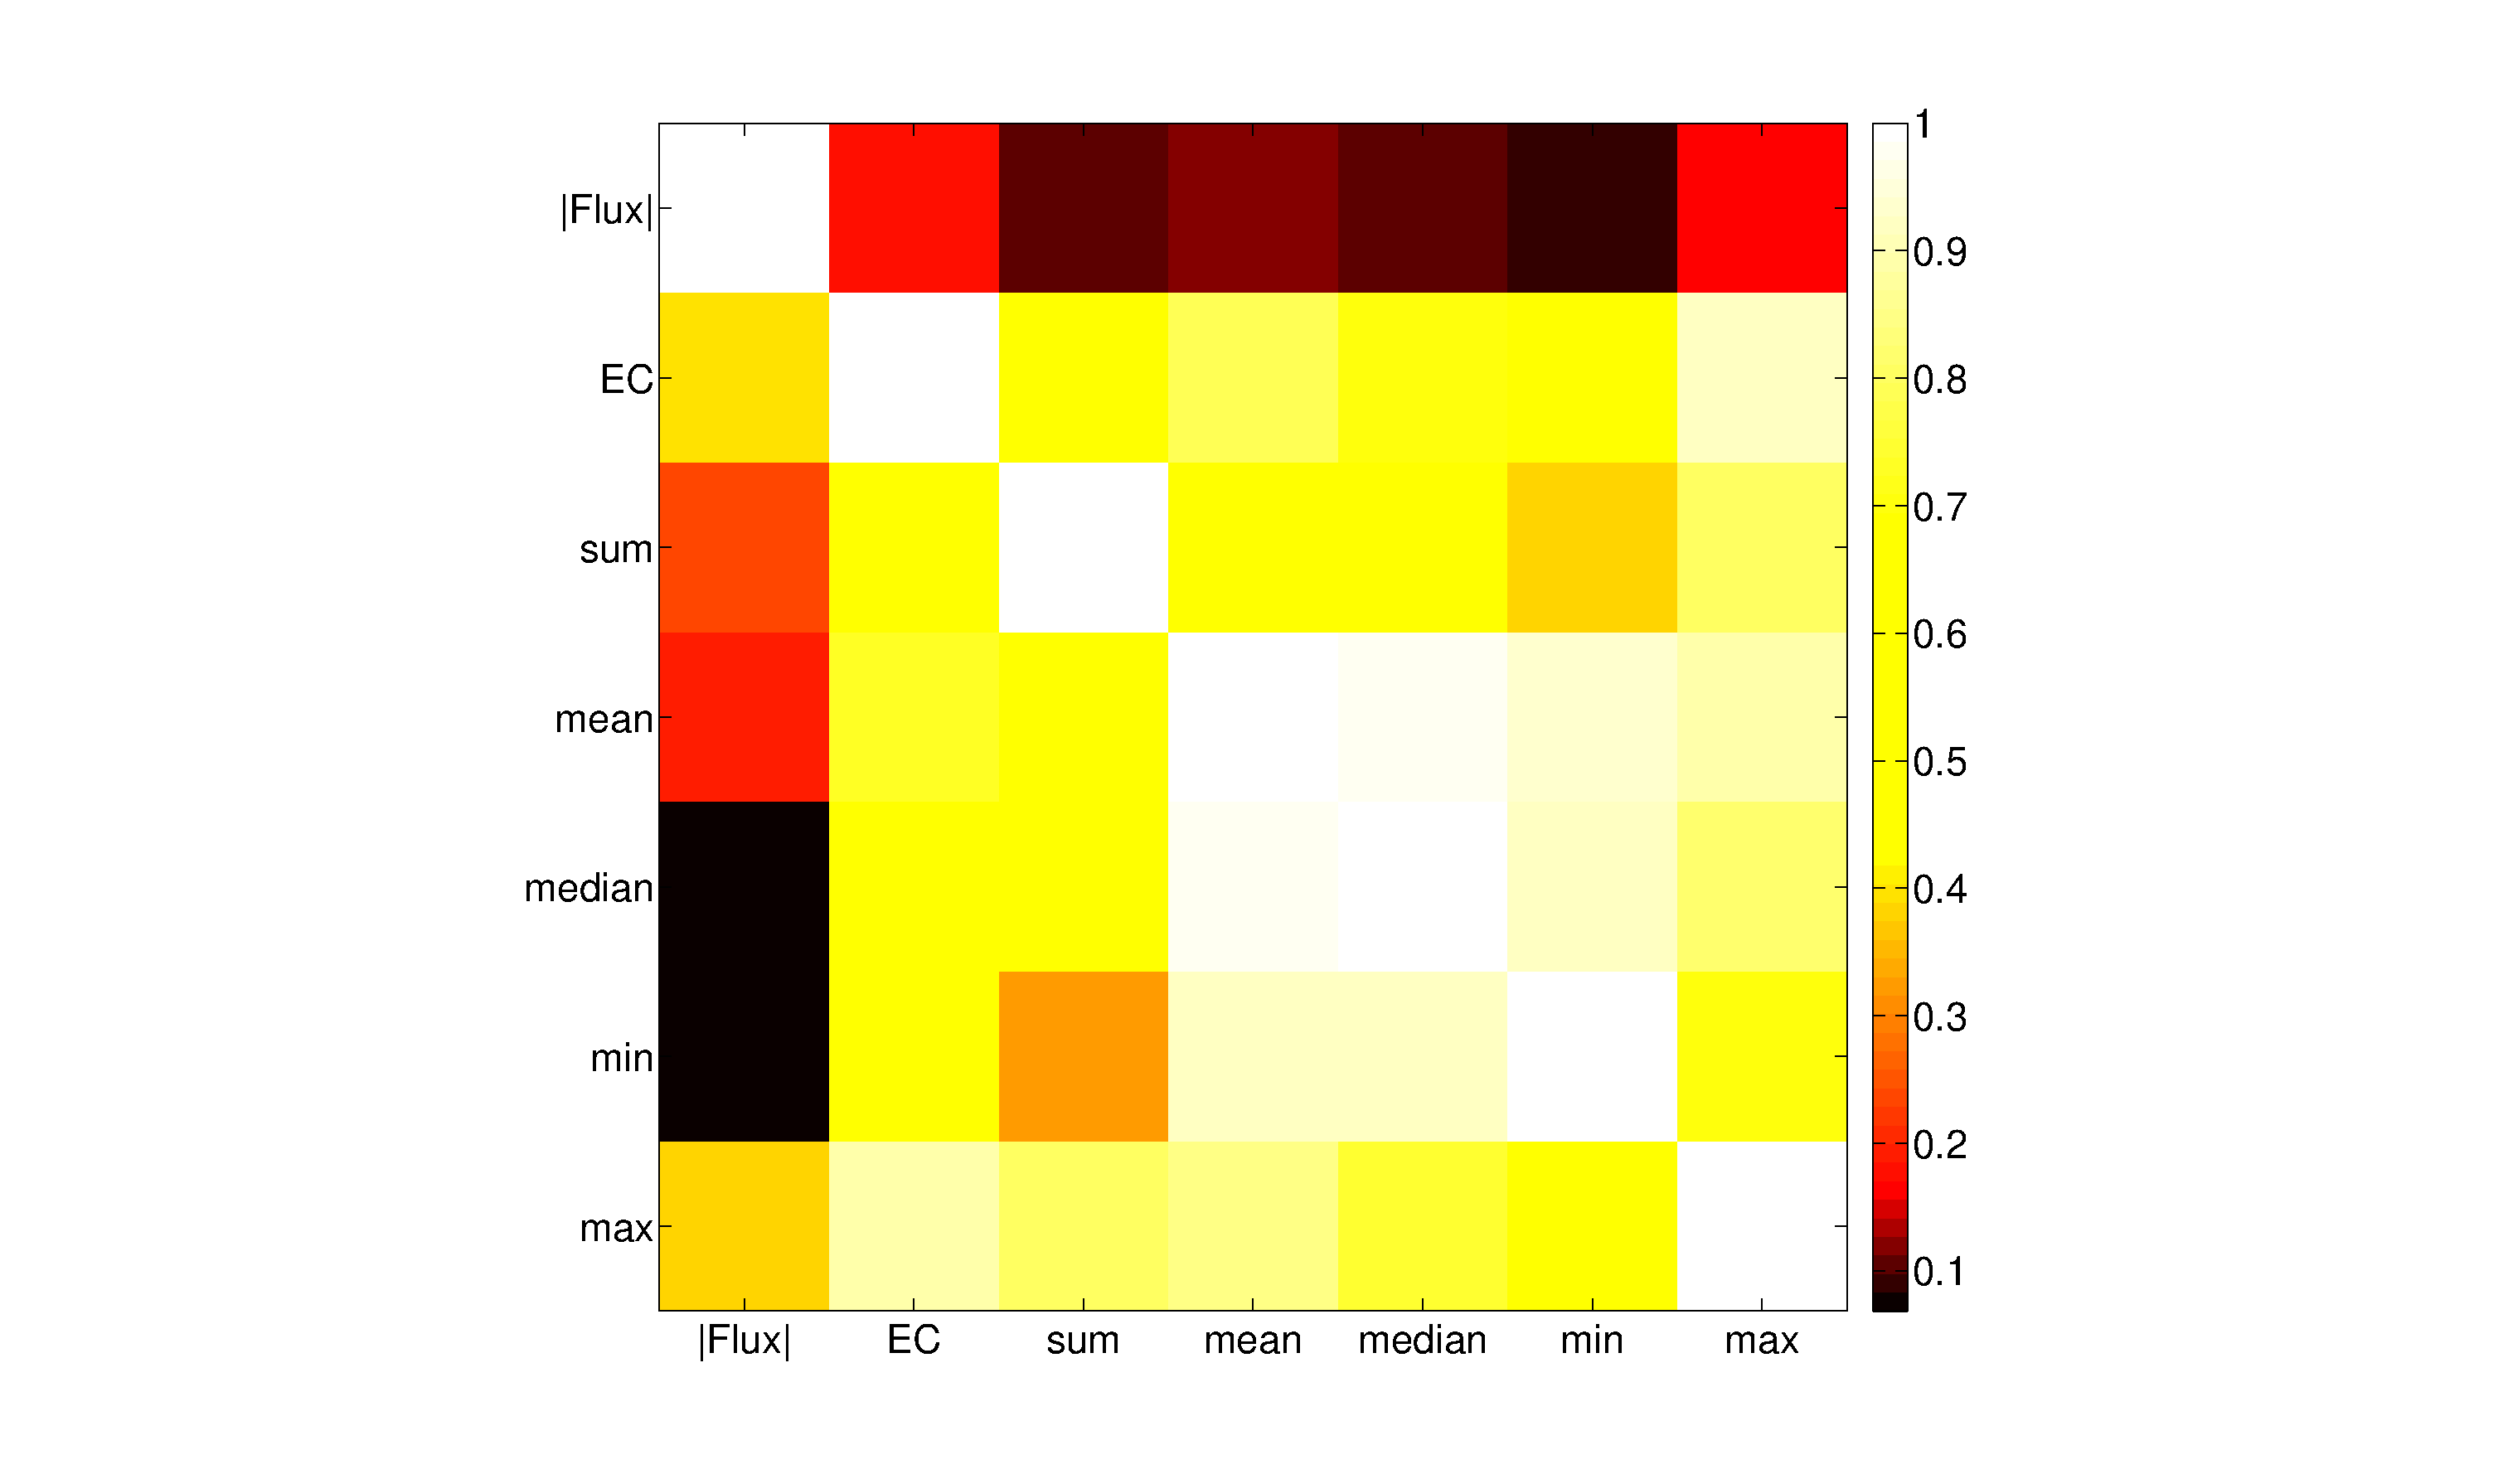
\includegraphics[width=\textwidth, trim=9cm 1.2cm 9cm 1cm, clip=true]
    {HumanExpFluxCompare}
  \caption{human} \label{fig:FluxExpCmp:B}
  \end{subfigure}
\\
\end{tabular}
\caption{Pearson correlation between FALCON flux magnitudes, and
various complex quantification estimates in yeast \textbf{(a)} and
human \textbf{(b)}.}
\label{fig:FluxExpCmp}
\end{figure}
}


%%%%%%%%%%%%%%%%%%%%%%%%%%%%%%%%%%%%%%%%%%%%%%%%%%%%%%%%%%%%%%%%%%%%%%%%%%%%%%%%%%%%%%%%%%

\frame{\frametitle{Flux estimates and empirical flux measurements in Yeast} 

\begin{figure}

\newdimen\fluxfigwidth
\fluxfigwidth=0.75\textwidth
\newdimen\fluxlegwidth
\fluxlegwidth=\textwidth
\advance\fluxlegwidth-\fluxfigwidth

\begin{tabular}{cc}
  \begin{subfigure}[lb]{\fluxfigwidth}
  \includegraphics<1>[width=\textwidth]{gluc75_bars}
  \includegraphics<2>[width=\textwidth]{eth75_bars}
  \includegraphics<3>[width=\textwidth]{co2_75_bars}
  \includegraphics<4>[width=\textwidth]{glycerol75_bars}
  \includegraphics<5>[width=\textwidth]{acetate75_bars}

%  \caption{\the\fluxfigwidth}
  \end{subfigure}
&
  \begin{subfigure}[lb]{\fluxlegwidth}
  \raisebox{0.3\height}{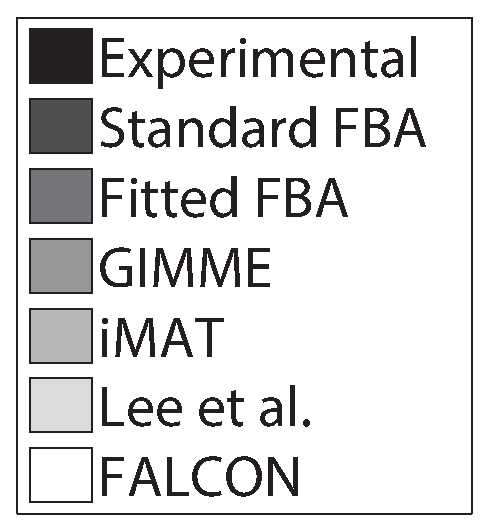
\includegraphics[scale=0.25,center]{legend_bars}}
%  \caption{\the\fluxlegwidth}
  \end{subfigure}
\\
\end{tabular}
\caption{\only<1>{glucose}\only<2>{ethanol}\only<3>{CO$_2$}%
\only<4>{glycerol}\only<5>{acetate}}

\end{figure}
}


%%%%%%%%%%%%%%%%%%%%%%%%%%%%%%%%%%%%%%%%%%%%%%%%%%%%%%%%%%%%%%%%%%%%%%%%%%%%%%%%%%%%%%%%%%
%%%%%%%%%%%%%%%%%%%%%%%%%%%%%% End Your Document %%%%%%%%%%%%%%%%%%%%%%%%%%%%%%%%%%%%%%%%%
%%%%%%%%%%%%%%%%%%%%%%%%%%%%%%%%%%%%%%%%%%%%%%%%%%%%%%%%%%%%%%%%%%%%%%%%%%%%%%%%%%%%%%%%%%

\end{document}

